\documentclass[12pt,english]{article}
\usepackage{natbib}
\usepackage{amsmath,mathtools,amssymb,mathrsfs,dsfont,amsthm}
\usepackage[margin=1in]{geometry}
\usepackage{algpseudocode}
\usepackage{algorithm}
\usepackage{caption}
\usepackage[T1]{fontenc}
\usepackage{babel}
\usepackage{graphicx}
\usepackage{float}
\usepackage{color}
\usepackage{subcaption}
\graphicspath{ {figures/} }
\usepackage[colorlinks]{hyperref}
\hypersetup{citecolor=blue}
\usepackage{enumitem}
\usepackage{authblk}
\usepackage{pifont}
\usepackage{lineno}
\usepackage[normalem]{ulem}

\renewcommand\Affilfont{\itshape\scriptsize}
\renewcommand\Authfont{\small}
\newcommand{\xmark}{\ding{55}}
%opening
\title{A semi-supervised Bayesian approach for simultaneous protein sub-cellular localisation assignment and organelle discovery }
\author[1,2]{Oliver M. Crook}
\author[1]{Lisa M. Breckels}
\author[1]{Aikaterini Geladaki}
\author[1]{Daniel J.H. Nightingale}
\author[1]{Owen Vennard}
\author[1]{Kathryn S. Lilley}
\author[2]{Paul D.W. Kirk\thanks{\url{paul.kirk@mrc-bsu.cam.ac.uk}}~}
\author[3]{Laurent Gatto\thanks{\url{laurent.gatto@uclouvain.be}}~}



\affil[1]{Cambridge Centre for Proteomics, Department of Biochemistry,
	University of Cambridge, Cambridge, UK}
\affil[2]{MRC Biostatistics Unit, Cambridge Institute for Public
	Health, Cambridge, UK}
\affil[3]{de Duve Institute, UCLouvain, Avenue
	Hippocrate 75, 1200 Brussels, Belgium}

\begin{document}

\maketitle

\begin{abstract}
The cell is compartmentalised into complex micro-environments allowing an array of
specialised biological processes to be carried out in synchrony. Determining a protein's sub-cellular localisation to one or more of these compartments can therefore be a first step in determining its function. High-throughput and high-accuracy mass spectrometry based sub-cellular proteomic methods can now shed light on the localisation of thousands of proteins at once. Machine learning algorithms are then typically employed to make protein-organelle assignments. However, these algorithms are limited by insufficient and incomplete annotation. We propose a semi-supervised Bayesian approach to novelty detection, allowing the discovery of additional, previously unannotated sub-cellular niches present within the data. Inference in our model is performed in a fully Bayesian framework, allowing us to quantify uncertainty in the allocation of proteins to new sub-cellular niches, as well as in the number of newly discovered compartments. We apply our approach across $10$ mass spectrometry based spatial proteomic datasets, representing a diverse repertoire of experimental protocols. Application of our approach to two \textit{hyper}LOPIT datasets validates its utility by recovering enrichment with chromatin-associated proteins without annotation. Novel compartmentalisation is uncovered in sub-cellular proteomics data on the U-2 OS cell line and this is validated by annotations from the Human Protein Atlas. Moreover, using data on \textit{Saccharomyces cerevisiae}, we uncover a collection of proteins trafficking from the ER to the early Golgi.
\end{abstract}
\clearpage
\section{Introduction}
Aberrant protein sub-cellular localisation has been implicated in numerous diseases, including cancers \citep{Kau:2004}, obesity \citep{Siljee:2018}, and multiple others \citep{Laurila:2009}. Furthermore, recent estimates suggest that up to $50\%$ of proteins reside in multiple locations with potentially different functions in each sub-cellular niche \citep{hyper, Thul:2017}. Characterising the sub-cellular localisation of proteins is therefore of critical importance in order to understand the pathobiological mechanisms and aetiology of many diseases. Proteins are compartmentalised into sub-cellular niches, including organelles, sub-cellular structures, liquid phase droplets and protein complexes. These compartments ensure the biochemical conditions for proteins to function correctly are met, and that they are in the proximity of intended interaction partners \citep{Gibson:2009}. High-throughput and high-accuracy mass spectrometry (MS)-based methods to map the global sub-cellular landscape now exist \citep{hyper, Mulvey:2017, DC:2018, Orre:2019}. These methods begin with gentle cell lysis, proceeded by sub-cellular fractionation and MS-based proteomics profiling. These spatial proteomics approaches rely on rigorous data analysis and interpretation \citep{Gatto:2010, Gatto:2014b}.

Current computational approaches in MS-based spatial proteomics rely on machine learning algorithms to make protein-organelle assignments (see \citep{Gatto:2014b} for an overview). If a dataset is insufficiently annotated, such that sub-cellular niches that are present in the experimental data are missing from the training dataset, then this leads to the classifier making erroneous assignments, resulting in inflated \textit{false discovery rate} (FDR) and uncertainty estimates (where available). Therefore, novelty detection, the process of identifying differences between testing and training data, and organelle discovery is of vital importance in spatial proteomics.

Novelty detection can also prove useful in validating experimental design, either by demonstrating contaminants have been removed or by increasing resolution of organelle classes. Furthermore, organisms for which we have little \textit{a priori} knowledge of their proteome organisation can be challenging to annotate and novelty detection can provide putative evidence for sufficient resolution. Since resolution is an important factor in deciding how the proteome should be annotated, \cite{Gatto:2018} proposed a quantitative measure of organelle resolution to guide users.

\cite{Breckels:2013} presented a phenotype discovery algorithm called \textit{phenoDisco} to detect novel sub-cellular niches and alleviate the issue of undiscovered phenotypes. The algorithm uses an iterative procedure and the \textit{Bayesian Information Criterion} (BIC) \citep{Schwarz::1978} is employed to determine the number of newly detected phenotypes. Afterwards, the dataset can be re-annotated and a classifier employed to assign proteins to organelles, including those that have been newly detected. \cite{Breckels:2013} applied their method on several datasets and discovered new organelle classes in \textit{Arabidopsis} \citep{Dunkley:2006} and \textit{Drosophila} \citep{Tan:2009}. This approach later successfully identified the trans-Golgi network (TGN) in \textit{Arabidopsis} roots \citep{Groen:2014}.

Recently, \cite{Crook:2018} demonstrated the importance of uncertainty quantification in spatial proteomics. They proposed a generative classification model and took a fully Bayesian approach to spatial proteomics data analysis by computing probability distributions of protein-organelle assignments using Markov-chain Monte-Carlo (MCMC). These probabilities were then used as the basis for organelle allocations, as well as to quantify the uncertainty in these allocations. On the basis that some proteins cannot be well described by any of the annotated sub-cellular niches, a multivariate student's T distribution was included for outlier detection. The proposed T-Augmented Gaussian Mixture (TAGM) model was shown to achieve state-of-the-art predictive performance against other commonly used machine learning algorithms \citep{Crook:2018}. 

Here, we propose an extension to TAGM to allow simultaneous protein-organelle assignments and novelty detection. One assumption of the existing TAGM model is that the number of organelle classes is known. Here, we design a novelty detection algorithm based on allowing an unknown number of additional organelle classes, as well as quantifying uncertainty in this number.

Quantifying uncertainty in the number of components in a Bayesian mixture model is challenging and many approaches have been proposed in the literature (see for example \cite{ferguson::1974, antoniak::1974, Richardson::1997} and the appendix for further details). Here, we make use of recent asymptotic results in Bayesian analysis of mixture models \citep{Rousseau::2011}. The principle of overfitted mixtures allows us to specify a (possibly large) maximum number of components. As shown in \cite{Rousseau::2011} these components empty if they are not supported by the data, allowing the number of components to be inferred. \cite{Kirk:2012} previously made use of this approach in the Bayesian integrative modelling of multiple genomic datasets. In our application, some of the organelles may be annotated with known marker proteins and this places a lower bound on the number of sub-cellular niches. Bringing these ideas together results in a semi-supervised Bayesian approach, which we refer to as Novelty TAGM. A schematic overview of the model is displayed in figure \ref{figure:overview}. 

We apply Novelty TAGM to $10$ spatial proteomic datasets across a diverse range of protocols, including \textit{hyper}LOPIT \citep{hyper, Mulvey:2017}, LOPIT-DC \citep{DC:2018}, Dynamic Organellar Maps (DOM) \citep{Itzhak:2016} and spatial-temporal methods \citep{Jean_Beltran:2016}. We first validate our approach by recovering the chromatin-associated protein cluster in \textit{hyper}LOPIT datasets, including data on the E14TG2a mouse embryonic stem cell (mESC) line and U-2 OS human bone osteosarcoma cells. Application of Novelty TAGM to each dataset reveal additional biologically relevant compartments. Notably, we demonstrate that the U-2 OS \textit{hyper}LOPIT dataset reveals $4$ sub-nuclear compartments: the nucleolus,  nucleoplasm, chromatin-associated, and the nuclear membrane. These findings are validated using the Human Protein Atlas \citep{Thul:2017,Sullivan:2018}. In addition, an endosomal compartment is robustly identified across \textit{hyper}LOPIT and LOPIT-DC datasets. We are also able to uncover small collections of proteins with previously uncharacterised localisation patterns; for example, we identify vesicle proteins trafficking from the ER to the early Golgi in a \textit{hyper}LOPIT data on \textit{Saccharomyces cerevisiae}.
\begin{figure}[h]
	
	\centering
	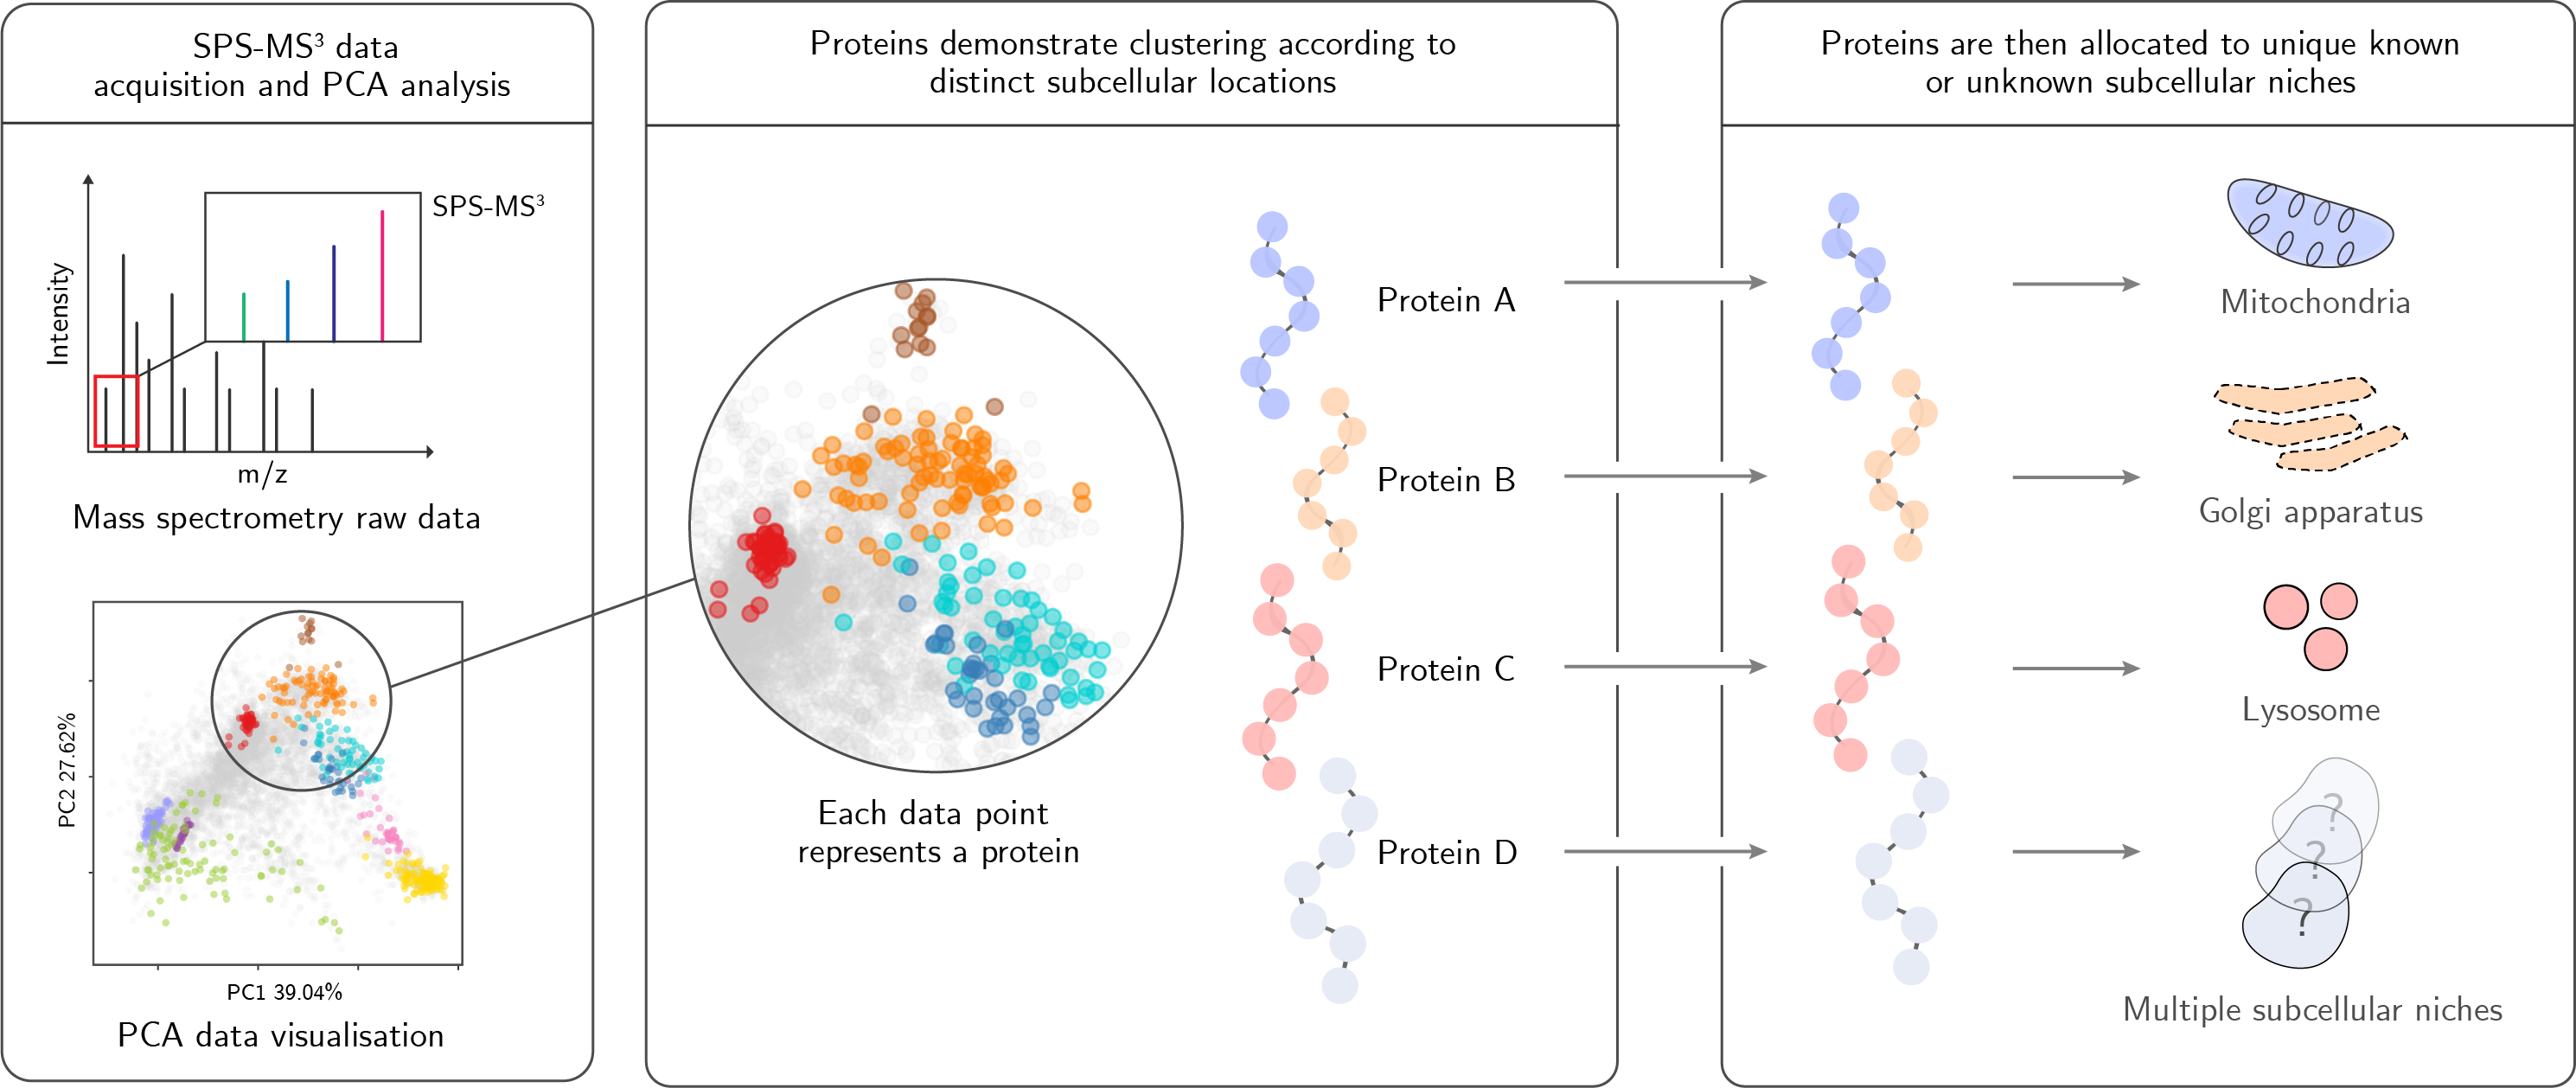
\includegraphics[height=2.8in]{IMG_Protein_Allocation_Draft_v1}
	\caption{An overview of the Novelty TAGM method.}
	\label{figure:overview}
\end{figure}

\section{Methods}
\subsection{Datasets}
We provide a brief description of the datasets used in this manuscript. We analyse \textit{hyper}LOPIT data, in which sub-cellular fractionation is performed using density-gradient centrifugation \citep{Dunkley:2004, Dunkley:2006, Mulvey:2017}, on pluripotent mESCs (E14TG2a) \citep{hyper}, human bone osteosarcoma (U-2 OS) cells \citep{Thul:2017, DC:2018}, and \textit{S. cerevisiae} (bakers' yeast) data \citep{Nightingale::2019}. The mESC dataset combines two 10-plex biological replicates and quantitative information on $5032$ proteins. The U-2 OS dataset combines three 20-plex biological replicates and provides information on $4883$ proteins. The yeast dataset represents four 10-plex biological replicate experiments performed on \textit{S. cerevisiae} cultured to early-mid exponential phase. This dataset contains quantitative information for $2846$ proteins that were common across all replicates. Tandem Mass Tag (TMT) \citep{Thompson:2003} labelling was used in all \textit{hyper}LOPIT experiments with LC-SPS-MS$^{3}$ used for high accuracy MS-based quantitation \citep{Ting:2011, Mcalister::2014}. \cite{Jean_Beltran:2016} integrated a temporal component to the LOPIT protocol. They analysed HCMV-infected primary fibroblast cells over 5 days, producing control and infected maps every 24 hours. We analyse the control and infected maps 24 hours post-infection, providing information on $2220$ and $2196$ proteins respectively. In a comparison with \textit{phenoDisco}, we apply Novelty TAGM to a dataset acquired using LOPIT-based fractionation and 8-plex iTRAQ labelling on the HEK-293 human embryonic kidney cell line, quantifying 1371 proteins \citep{Breckels:2013}.

Our approach is not limited to spatial proteomics data where the sub-cellular fractionation is performed using density gradients. We demonstrate this through the analysis of DOM datasets on HeLa cells and mouse primary neurons \citep{Itzhak:2016, Itzhak::2017}, which quantify $3766$ and $8985$ proteins respectively. These approaches used label-free quantitation with differential centrifugation-based fractionation. We analyse $6$ replicates from the HeLa cell line analyses in \cite{Itzhak:2016} and $3$ replicates from the mouse primary neuron experiments in \cite{Itzhak::2017}. \cite{Hirst:2018} also used the DOM protocol coupled with CRISPR-CAS9 knockouts in order to explore the functional role of AP-5. We analyse the control map from this experiment. Finally, we consider the U-2 OS data which were acquired using LOPIT-DC protocol \citep{DC:2018} and quantified $6837$ across $3$ biological replicates. Though we do not consider protein correlation profiling (PCP) based spatial proteomics datasets in this manuscript, our method also applies to such data \citep{Foster:2006, kristensen:2012, kristensen:2014} and other sub-cellular proteomics methods \citep{Orre:2019}.
\subsection{Model}
\subsubsection{Spatial proteomics mixture model}
In this section, we briefly review the TAGM model proposed by \citep{Crook:2018}. Let $N$ denote the number of observed protein profiles each of length $L$, corresponding to
the number of quantified fractions. The quantitative profile for the $i$-th protein is denoted by ${\bf x}_i = [x_{1i}, \ldots, x_{Li}]$.  In the original formulation of the model it is supposed that there are $K$
known sub-cellular compartments to which each protein could be localise
(e.g. cytosol, endoplasmic reticulum, mitochondria, \ldots). For simplicity of exposition, we refer to these $K$ sub-cellular compartments as {\em
	components}, and introduce component labels $z_i$, so that $z_i = k$
if the $i$-th protein localises to the $k$-th component. To fix notation, we denote by
$X_L$ the set of proteins whose component labels are known, and by
$X_U$ the set of unlabelled proteins.  If protein $i$ is in $X_U$, we
want the probability that $z_i = k$ for each $k = 1, \ldots, K$;
that is, for each unlabelled protein, the probability of
belonging to each component (given a model and the observed data).


The distribution of quantitative profiles associated with each
protein that localise to the $k$-th component is modelled as multivariate normal
with mean vector $\boldsymbol{\mu}_k$ and covariance matrix
$\Sigma_k$. However, many proteins are dispersed and do not fit this assumption. To model these "outliers", \cite{Crook:2018} introduced a further indicator variable $\phi$. Each protein ${\bf x}_i$ is then described by an additional variable $\phi_i$, with $\phi_i = 1$ indicating that protein ${\bf x}_i$ belongs to an
organelle-derived component and $\phi_i = 0$ indicating that protein
${\bf x}_i$ is not well described by these known components. This
outlier component is then modelled as a multivariate T distribution with
degrees of freedom $\kappa$, mean vector $\bf{M}$, and scale matrix
$V$. Thus the model can be written as:

\begin{align}
{\bf x}_i | z_i = k, \phi_i \quad \sim \mathcal{N}(\boldsymbol{\mu}_k, \Sigma_k)^{\phi_i}\mathcal{T}(\kappa, \boldsymbol{M}, V)^{1 - \phi_i }.
\end{align}


Let  $f({\bf x} | \boldsymbol{\mu}, \Sigma)$ denote the density of
the multivariate normal with mean vector $\boldsymbol{\mu}$ and
covariance matrix $\Sigma$ evaluated at ${\bf x}$ and $g({\bf x | \kappa, \bf{M}, V} )$ denote the density of the multivariate T-distribution. For any $i$, the prior probability of the $i$-th protein localising to the $k$-th component is denoted by $p(z_i = k) = \pi_k$. Letting
$\boldsymbol{\theta} = \{\boldsymbol{\mu}_k, \Sigma_k \}_{k = 1}^K$
denote the set of all component mean and covariance parameters, and
$\boldsymbol{\pi} = \{\pi_k\}_{k = 1}^K$ denote the set of all mixture
weights, it follows that:

\begin{equation} \label{equation::tammeq}
\begin{split}
p({\bf x}_i| \boldsymbol{\theta}, \boldsymbol{\pi} ,\phi_i, \kappa, {\bf M}, V) &=  \sum_{k=1}^{K}\pi_k\left(f({\bf x}_i|\boldsymbol{\mu}_k, \Sigma_k)^{\phi_i}g({\bf x}_i|\kappa, \boldsymbol{M}, V)^{1 - \phi_i }\right).\\
\end{split}
\end{equation}

For any $i$, we set the prior probability of the $i$-th protein
belonging to the outlier component as $p(\phi_i = 0) = \epsilon$.

Equation \eqref{equation::tammeq}  can then be rewritten in the following way:

\begin{equation}\label{equation::tammepseq}
\begin{split}
p({\bf x}_i| \boldsymbol{\theta}, \boldsymbol{\pi} , \kappa, \epsilon, {\bf M}, V) &=  \sum_{k=1}^{K}\pi_k\left((1-\epsilon)(f({\bf x}_i |\boldsymbol{\mu}_k, \Sigma_k) + \epsilon g({\bf x}_i|\kappa, \boldsymbol{M}, V)\right),\\
\end{split}
\end{equation}

As in \cite{Crook:2018}, we fix $\kappa = 4$, ${\bf M}$ as the global empirical mean, and $V$
as half the global empirical variance of the data, including labelled and unlabelled proteins. To extend this model to permit novelty detection, we specify the maximum number of components $K_{max} > K$. Our proposed model then allows up to $K_{novelty} = K_{max} - K \geq 0$, new phenotypes to be detected. Equation \ref{equation::tammepseq} can then be written as 
\begin{equation}\label{equation::tammepseq2}
\begin{split}
p({\bf x}_i| \boldsymbol{\theta}, \boldsymbol{\pi} , \kappa, \epsilon, {\bf M}, V) =  \sum_{k=1}^{K}&\pi_k\left((1-\epsilon)(f({\bf x}_i |\boldsymbol{\mu}_k, \Sigma_k) + \epsilon g({\bf x}_i|\kappa, \boldsymbol{M}, V)\right)\\
+ & \sum_{k=K+1}^{K_{max}}\pi_k\left((1-\epsilon)(f({\bf x}_i |\boldsymbol{\mu}_k, \Sigma_k) + \epsilon g({\bf x}_i|\kappa, \boldsymbol{M}, V)\right),
\end{split}
\end{equation}
where, in the first summation, the $K$ components correspond to known sub-cellular niches and the second summation corresponds to the new phenotypes to be inferred. The parameter sets are then augmented to include these possibly new components; that is, we redefine 
$\boldsymbol{\theta} = \{\boldsymbol{\mu}_k, \Sigma_k \}_{k = 1}^{K_{max}}$
to denote the set of all component mean and covariance parameters, and
$\boldsymbol{\pi} = \{\pi_k\}_{k = 1}^{K_{max}}$ denotes the set of all mixture
weights. Relying on the principle of over-fitted mixtures \cite{Rousseau::2011}, components that are not supported by the data are left empty with no proteins allocated to them. We find setting $K_{novety} = 10$ is ample to detect new phenotypes.   
\subsubsection{Bayesian inference and convergence}
We perform fully Bayesian inference, using Markov-chain Monte-Carlo methods. We make modifications to the collapsed Gibbs sampler approach used previously in \cite{Crook:2018} to allow inference to be performed for the parameters of the novel components (see supplement for full details). Since the number of occupied components at each iteration is random, we can monitor this quantity as a convergence diagnostic. At convergence the number of occupied components is not necessarily fixed, but oscillates around a fixed mode.
\subsubsection{Visualising patterns in uncertainty}
To simultaneously visualise the uncertainty in the number of newly discovered phenotypes, as well as the uncertainty in the allocation of proteins to new components, we use the so-called \textit{posterior similarity matrix} (PSM) \citep{fritsch::2009}. The PSM is an $N\times N$ matrix where the $(i,j)^{th}$ entry is the posterior probability that protein $i$ and protein $j$ reside in the same component. Throughout we use a heatmap representation of this quantity. The PSM is summarised into a clustering by maximising the posterior expected adjusted Rand index (see appendix for details)\citep{fritsch::2009}. Formulating inference around the PSM also avoids some technical statistical challenges, which are discussed in detail in the appendix.

\subsubsection{Uncertainty Quantification}
We may be interested in quantifying the uncertainty in whether a protein belongs to a new sub-cellular component. Indeed, it is important to distinguish whether a protein belongs to a new phenotype or if we simply have large uncertainty about its localisation. The probability that protein $i$ belongs to a new component is computed from the following equation:
\begin{align}
P(z_i \in \{K + 1,..., K_{max}\}|X) & = 1 - P(z_i \in \{1,..., K\}|X), \\ 
\end{align}
which we can approximate by the following Monte-Carlo average:
\begin{align}\label{equation::discoveryprob}
1 - \frac{1}{T} \sum_{t = 1}^{T}P(z^{(t)}_i \in \{1,..., K\}|X)= 1 - \frac{1}{T} \sum_{t = 1}^{T} \sum_{k=1}^KP(z^{(t)}_i = k|X)
\end{align}
Since the summation in equation \ref{equation::discoveryprob} only goes up to $K$ (the number of annotated organelles), this equation is identifiable. Throughout we refer to this as the discovery probability.
\subsection{Validating computational approaches}
In a supervised framework the performance of computational methods can be assessed by 
using the training data, where a proportion of the training data is withheld from the classifier to be used for the assessment of predictive performance. In an unsupervised or semi-supervised framework we cannot validate in this way, since there is no ground truth with which to compare. Thus, we propose three approaches, using external information, for independent validation of our method. Table \ref{table:methods} summarises the differences between the current available machine-learning methods for spatial proteomics.
\subsubsection{Artificial masking of annotations to recover experimental design}
Removing the annotations from an entire component and assessing the ability of our method to rediscover these annotations is one form of validation. We consider this validation approach for several of the datasets; in particular, chromatin enrichment was performed in two of the \textit{hyper}LOPIT experiments, where the intention was to increase the resolution between chromatin and non-chromatin associated nuclear proteins \citep{hyper, Mulvey:2017, DC:2018}. As validation of our method we hide these annotations and rediscover them in a unbiased fashion.
\subsubsection{The Human Protein Atlas}
A further approach to validating our method is to use orthogonal spatial proteomic information. The Human Protein Atlas \citep{Thul:2017, Sullivan:2018} provides confocal microscopy information on thousands of proteins, using validated antibodies. When we consider a dataset for which there is HPA annotation, we use this data to validate the novel phenotypes for biological relevance. 
\subsubsection{Gene Ontology (GO) term enrichment}
The Gene Ontology (GO) provides a database of relationships between genes and classes according to similar functional annotation. One of these annotations is Cellular Component which we exploit in our analysis. Throughout, we perform GO enrichment analysis with FDR control performed according to the Benjamini-H\"ochberg procedure \citep{FDR:1995,Ashburner:2000,Yu:2012}. The proteins in each novel phenotype are assessed in turn for enriched Cellular Component terms, against the background of all quantified proteins in that experiment. 

\begin{table}[h]
	\centering
	\footnotesize
	\hspace*{-1.5cm}
	\begin{tabular}{ |p{2.5cm}|p{2cm}|p{2cm}|p{1.5cm}|p{2cm}|p{2cm}|p{2cm}|p{2cm}|  }
		\hline
		\multicolumn{8}{|c|}{MS-based Spatial Proteomics Computational Methods} \\
		\hline
		 Method & Localisation prediction & Uncertainty in protein localisation & Outlier detection  & Novelty detection & Uncertainty in number of novel phenotypes & Uncertainty in allocation to new phenotypes & Integrative \\
		\hline
		\hline
		Supervised Machine Learning\citep{Gatto:2014b}  & \vfill\hfil \checkmark & \vfill\hfil\xmark & \vfill\hfil\xmark &\vfill\hfil\xmark&\vfill\hfil\xmark&\vfill\hfil\xmark& \vfill\hfil\xmark\\
		\hline
		Transfer Learning \citep{Breckels:2016}  & \vfill\hfil \checkmark  & \vfill\hfil\xmark& \vfill\hfil\xmark &\vfill\hfil\xmark&\vfill\hfil\xmark& \vfill\hfil\xmark&\vfill\hfil \checkmark\\
		\hline
		\textit{PhenoDisco} \citep{Breckels:2013}  & \vfill\hfil\xmark &\vfill\hfil\xmark &\vfill\hfil \checkmark &\vfill\hfil \checkmark&\vfill\hfil\xmark&\vfill\hfil\xmark& \vfill\hfil\xmark\\
		\hline
		TAGM \citep{Crook:2018}& \vfill\hfil \checkmark & \vfill\hfil \checkmark & \vfill\hfil \checkmark& \vfill\hfil\xmark&\vfill\hfil\xmark&\vfill\hfil\xmark&\vfill\hfil\xmark\\
		\hline
		Novelty TAGM (This manuscript)&  \vfill\hfil \checkmark & \vfill\hfil \checkmark &\vfill\hfil \checkmark & \vfill\hfil \checkmark&\vfill\hfil \checkmark&\vfill\hfil \checkmark& \vfill\hfil\xmark\\
		\hline
		\hline
	\end{tabular}
	\caption{Summary of computational methods for spatial  proteomics datasets.}
	\label{table:methods}
\end{table}
\clearpage
\section{Results}
\subsection{Validating experimental design in \textit{hyper}LOPIT}
To validate Novelty TAGM, we apply our method to a mESC \textit{hyper}LOPIT dataset \citep{hyper} and a recent human bone osteosarcoma cell (U-2 OS) \textit{hyper}LOPIT dataset \citep{Thul:2017, DC:2018}. These experimental protocols used a chromatin enrichment step to resolve nuclear chromatin-associated proteins from nuclear proteins not associated with the chromatin. Removing the nuclear, chromatin and ribosomal annotations from the datasets, we test the ability of Novelty TAGM to recover them.

\subsubsection{Pluripotent mESCs (E14TG2a)}
For the mESC dataset, Novelty TAGM reveals $8$ new phenotypes, which we refer to as phenotype 1, phenotype 2, etc., for which there is at least 1 protein with discovery probability greater than $0.95$. Novelty TAGM recovers these hidden annotations with phenotype $2$ having the enriched terms associated with chromatin, such as \textit{chromatin} and \textit{chromosome} $(p < 10^{-80})$. Phenotype 3 corresponds to a separate nuclear substructure with enrichment for the terms \textit{nucleolus} $(p < 10^{-60})$ and \textit{nuclear body} $(p < 10^{-30})$. Thus, in the mESC dataset Novelty TAGM confirms the chromatin enrichment preparation designed to separate chromatin and non-chromatin associated nuclear proteins \citep{Mulvey:2017}. In addition, phenotype 4 demonstrates enrichment for the ribosome annotation $(p < 10^{-35})$. Phenotype 1 is enriched for \textit{centrosome} and \textit{microtubule} annotations $(p < 10^{-15})$, though observing the PSM in figure \ref{figure:mouse} we can see there is much uncertainty in this phenotype. This uncertainty quantification can then be used as a basis for justifying additional expert annotation.

\subsubsection{The human bone osteosarcoma (U-2 OS) cells}
Now turning to the U-2 OS cancer cell line dataset, Novelty TAGM reveals $9$ new phenotypes for which there is at least 1 protein with a greater discovery probability than $0.95$. These phenotypes, along with the uncertainty associated with them, are visualised in figure \ref{figure:mouse}. We consider the HPA confocal microscopy data for validation \citep{Thul:2017, Sullivan:2018}. The HPA provides information on the same cell line and therefore constitutes an excellent complementary resource. This \textit{hyper}LOPIT dataset was already shown to be in strong agreement with the microscopy data \citep{Thul:2017, DC:2018}. Proteins in phenotypes $3,4,5$ and $8$ have a nucleus-related annotation as their most frequent annotation in the HPA data. Then, GO term enrichment analysis reveals \textit{chromatin} and \textit{chromosome} annotations for phenotype 3 $(p < 10^{-40})$. Phenotype $4$ is enriched for the \textit{nucleolus} $(p < 10^{-60})$, furthermore nucleoli and nucleoli/nucleus are the $2^{nd}$ and $3^{rd}$ most frequent HPA annotations for proteins belonging to this phenotype. For phenotype 5, the most associated term is nucleoplasm from the HPA data, as well as GO term enrichment $(p < 10^{-10})$. Phenotype $8$ has the \textit{nuclear membrane} as its most frequent HPA annotation and this is supported by GO term enrichment with the terms \textit{nuclear membrane} and \textit{nuclear envelope} associated with proteins in this phenotype $(p < 10^{-10})$. Thus, Novelty TAGM has not only provided successful validation for chromatin enrichment, but also demonstrated further sub-nuclear-level resolution. In addition, phenotype $1$ is enriched for \textit{ribosome} $( p < 10^{-20})$, whilst phenotype $2$ is enriched for \textit{endosomes} $(p < 10^{-30})$.


\begin{figure}[ht]
	\begin{subfigure}[t]{0.5\textwidth}
		\centering
		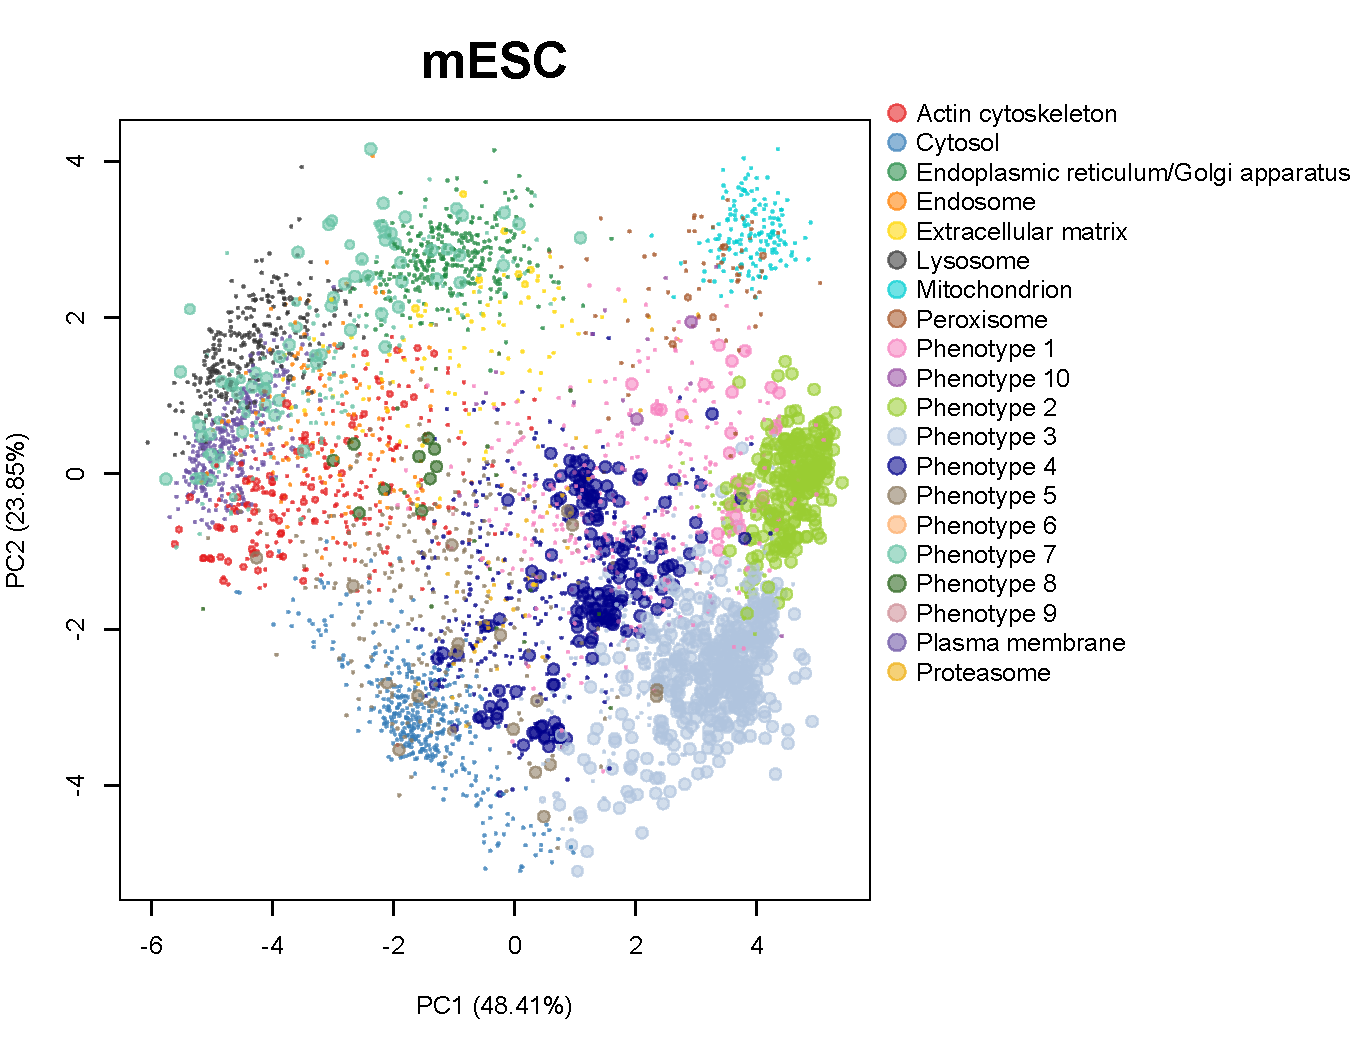
\includegraphics[height=2.5in]{pcaMousehl.pdf}
		\caption{}
	\end{subfigure}
	\begin{subfigure}[t]{0.5\textwidth}
		\centering
		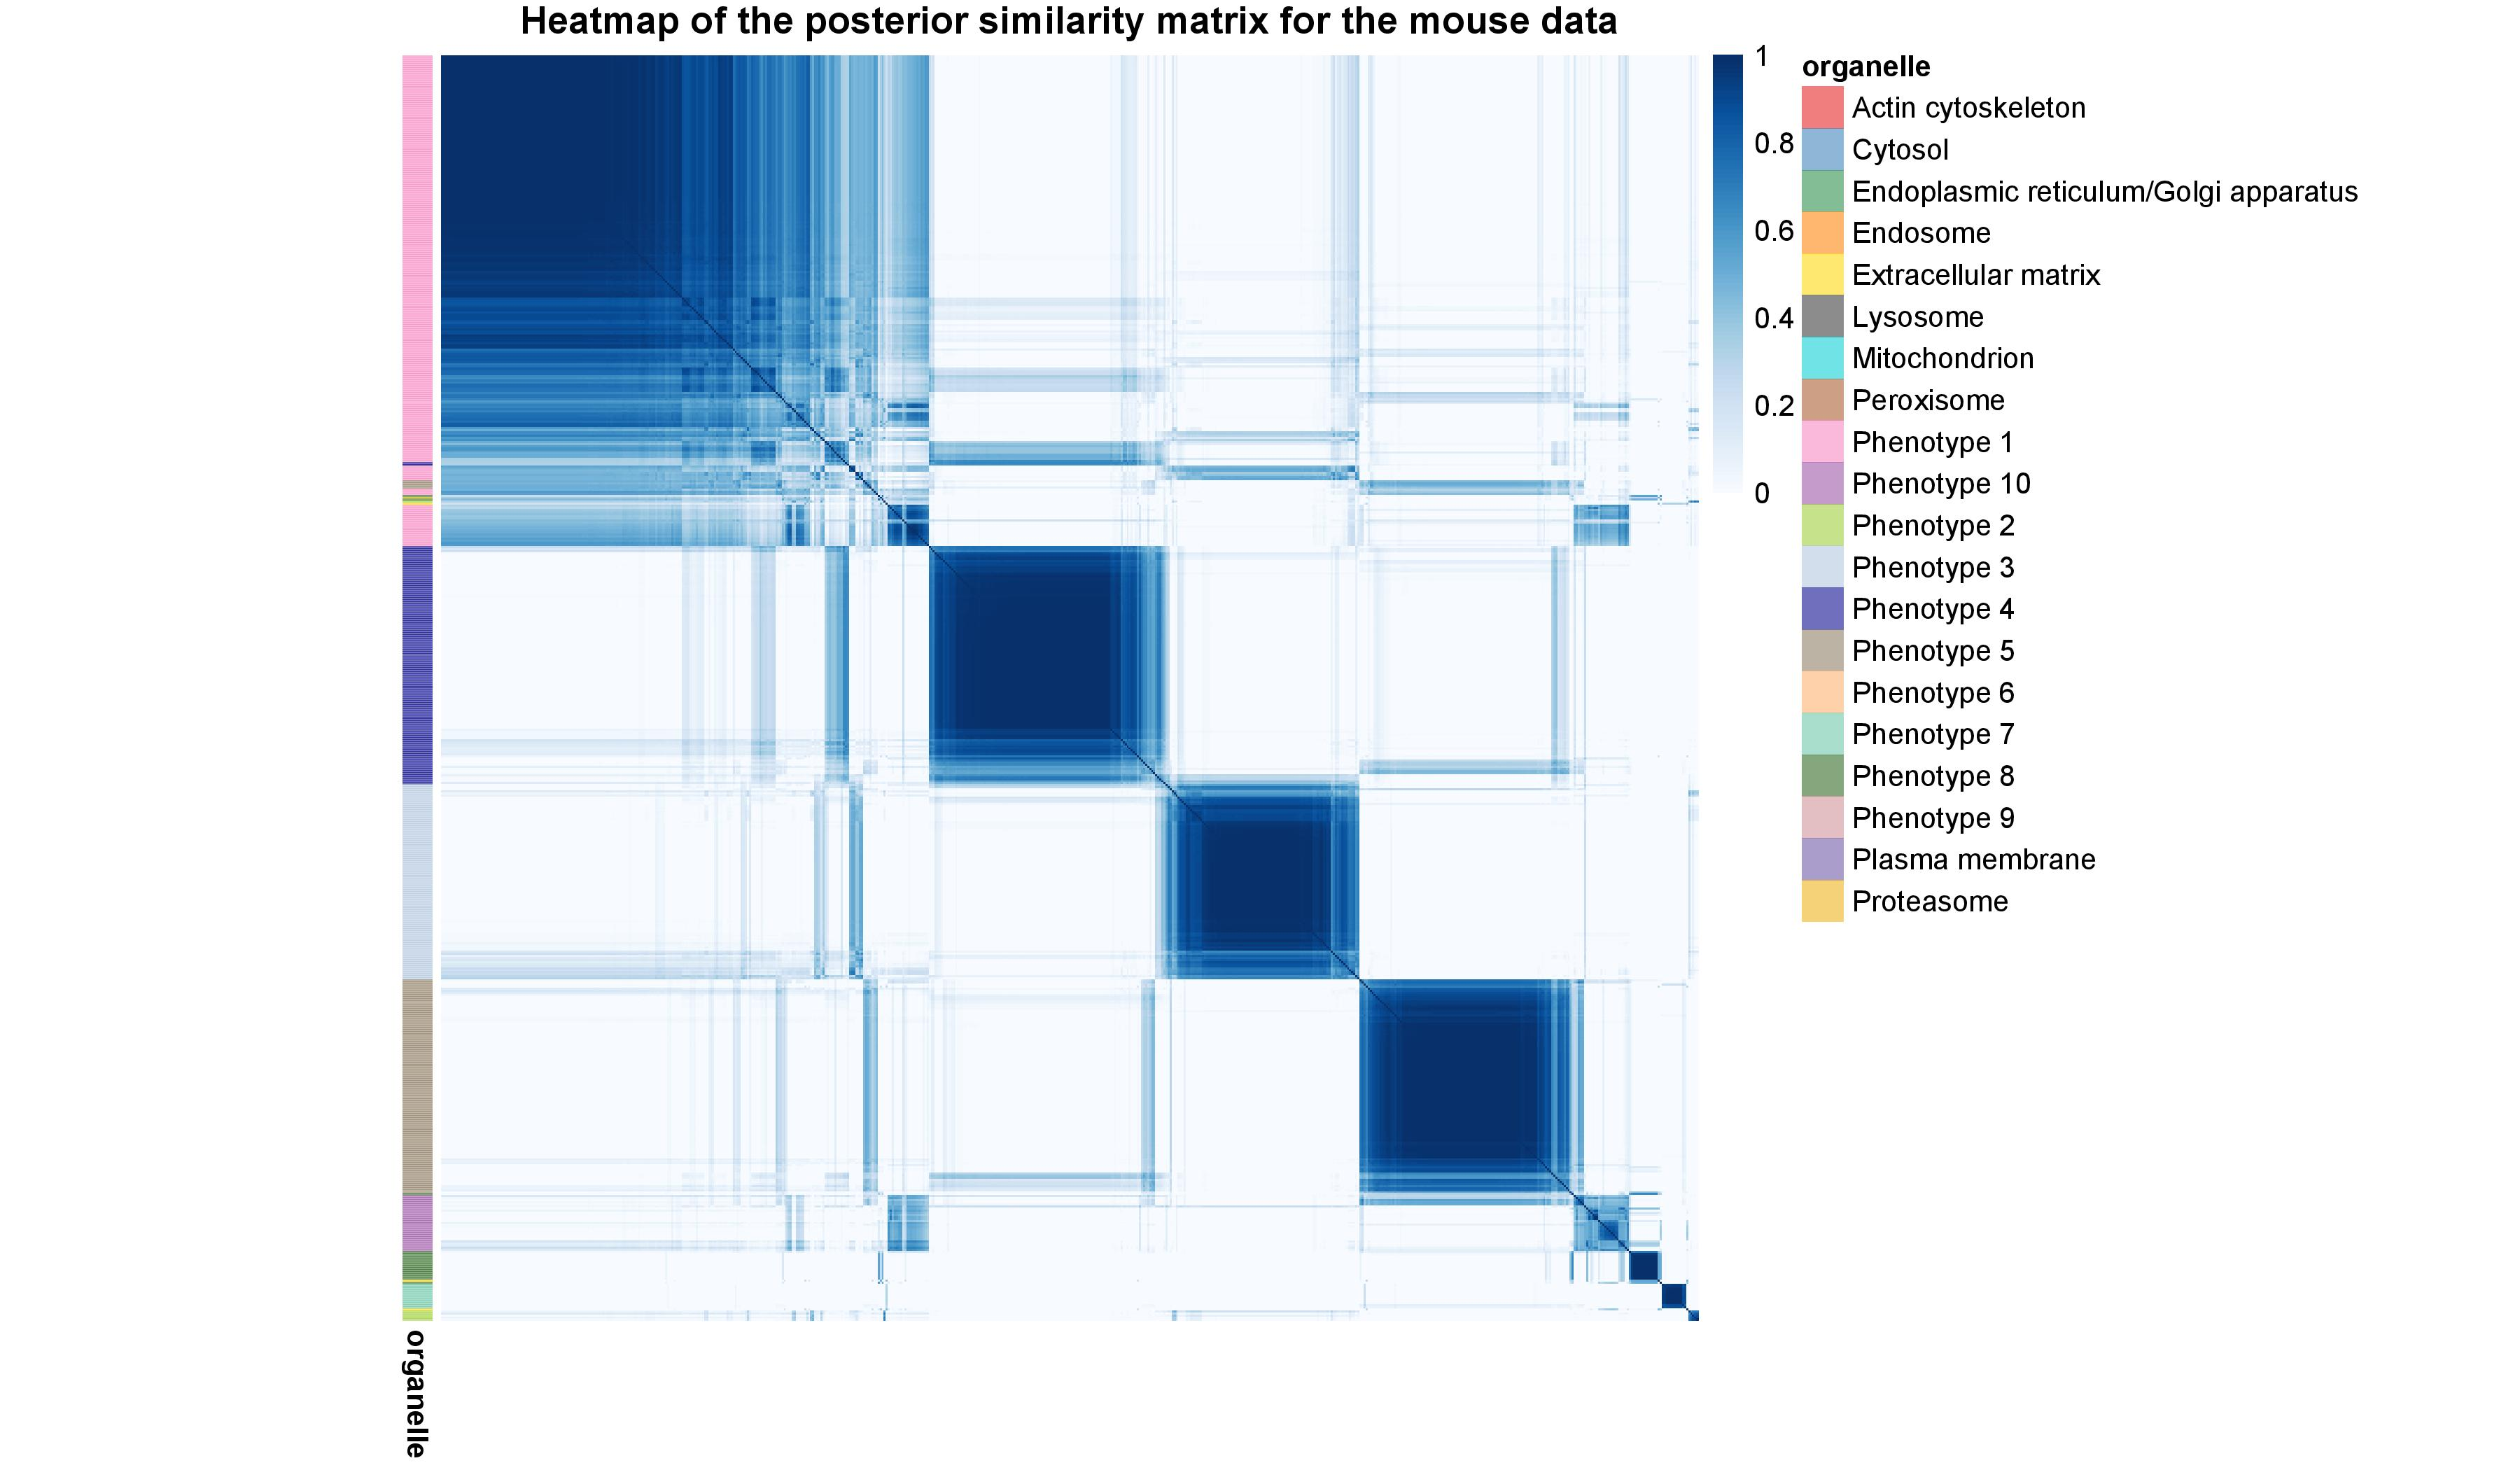
\includegraphics[height=2.5in]{heatmapMousehl.jpg}
		\caption{}
	\end{subfigure}
~
	\begin{subfigure}[t]{0.5\textwidth}
	\centering
	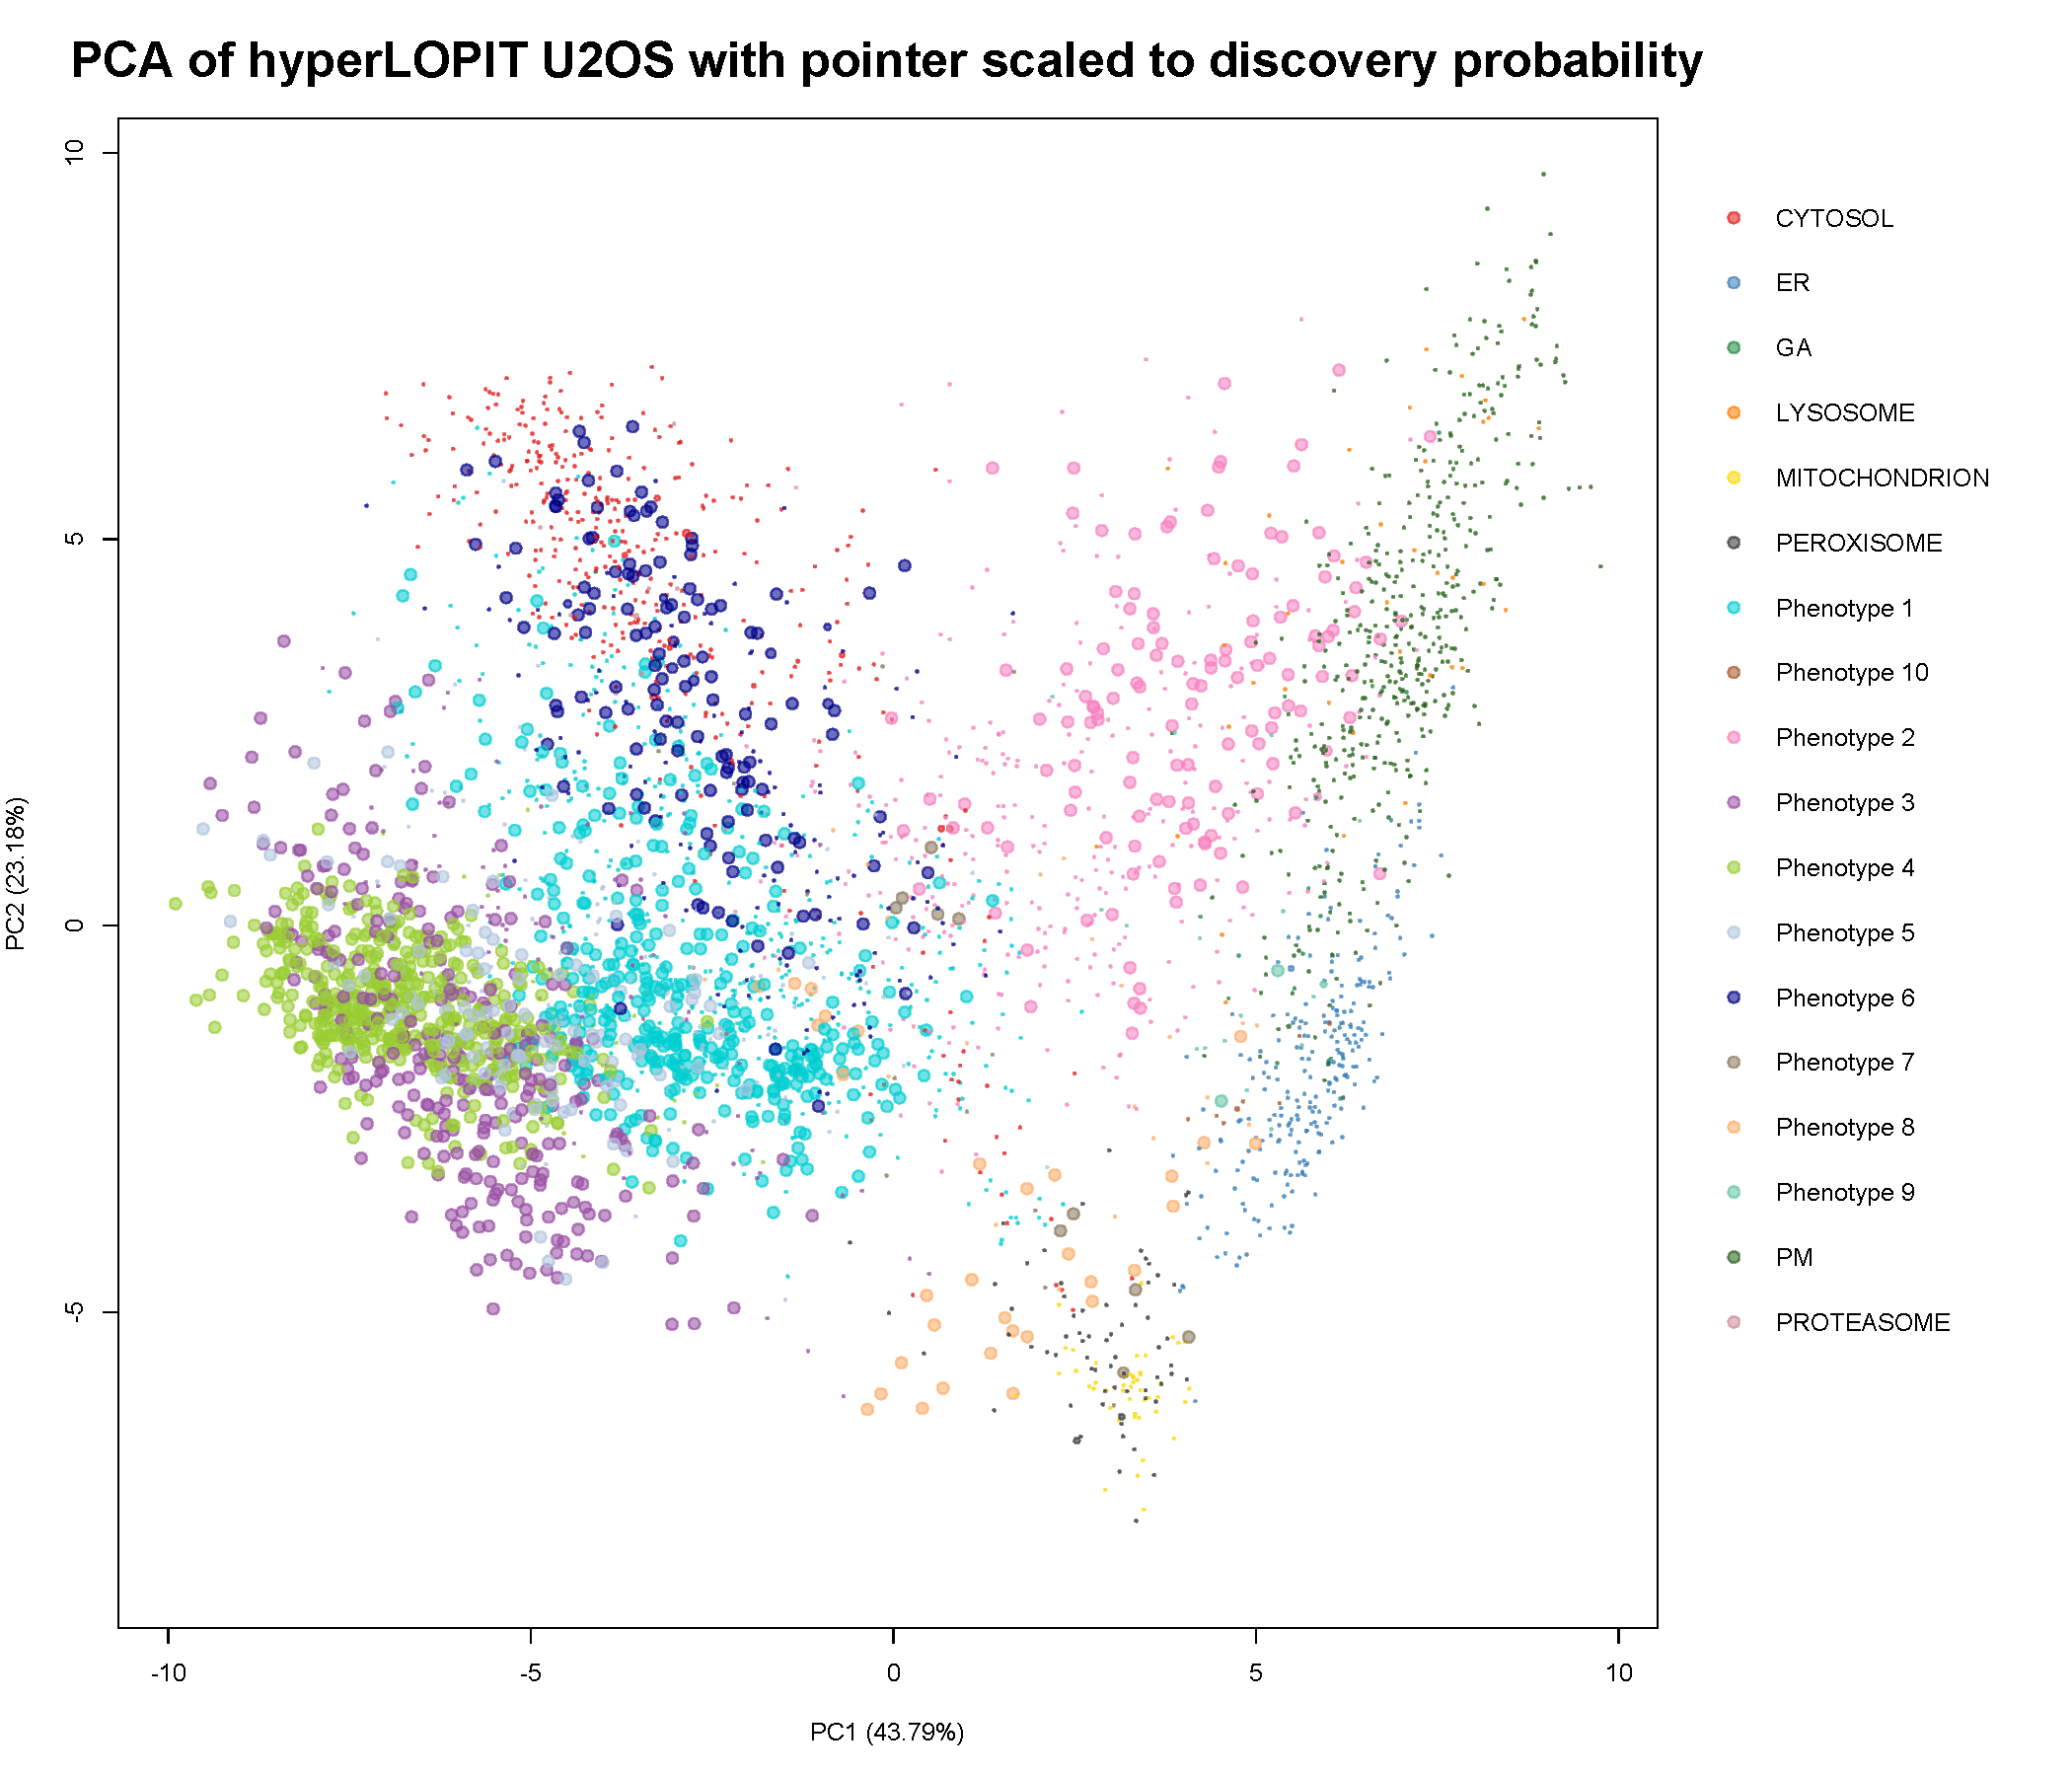
\includegraphics[height=2.5in]{pcau2oshl.pdf}
	\caption{}
\end{subfigure}
\begin{subfigure}[t]{0.5\textwidth}
	\centering
	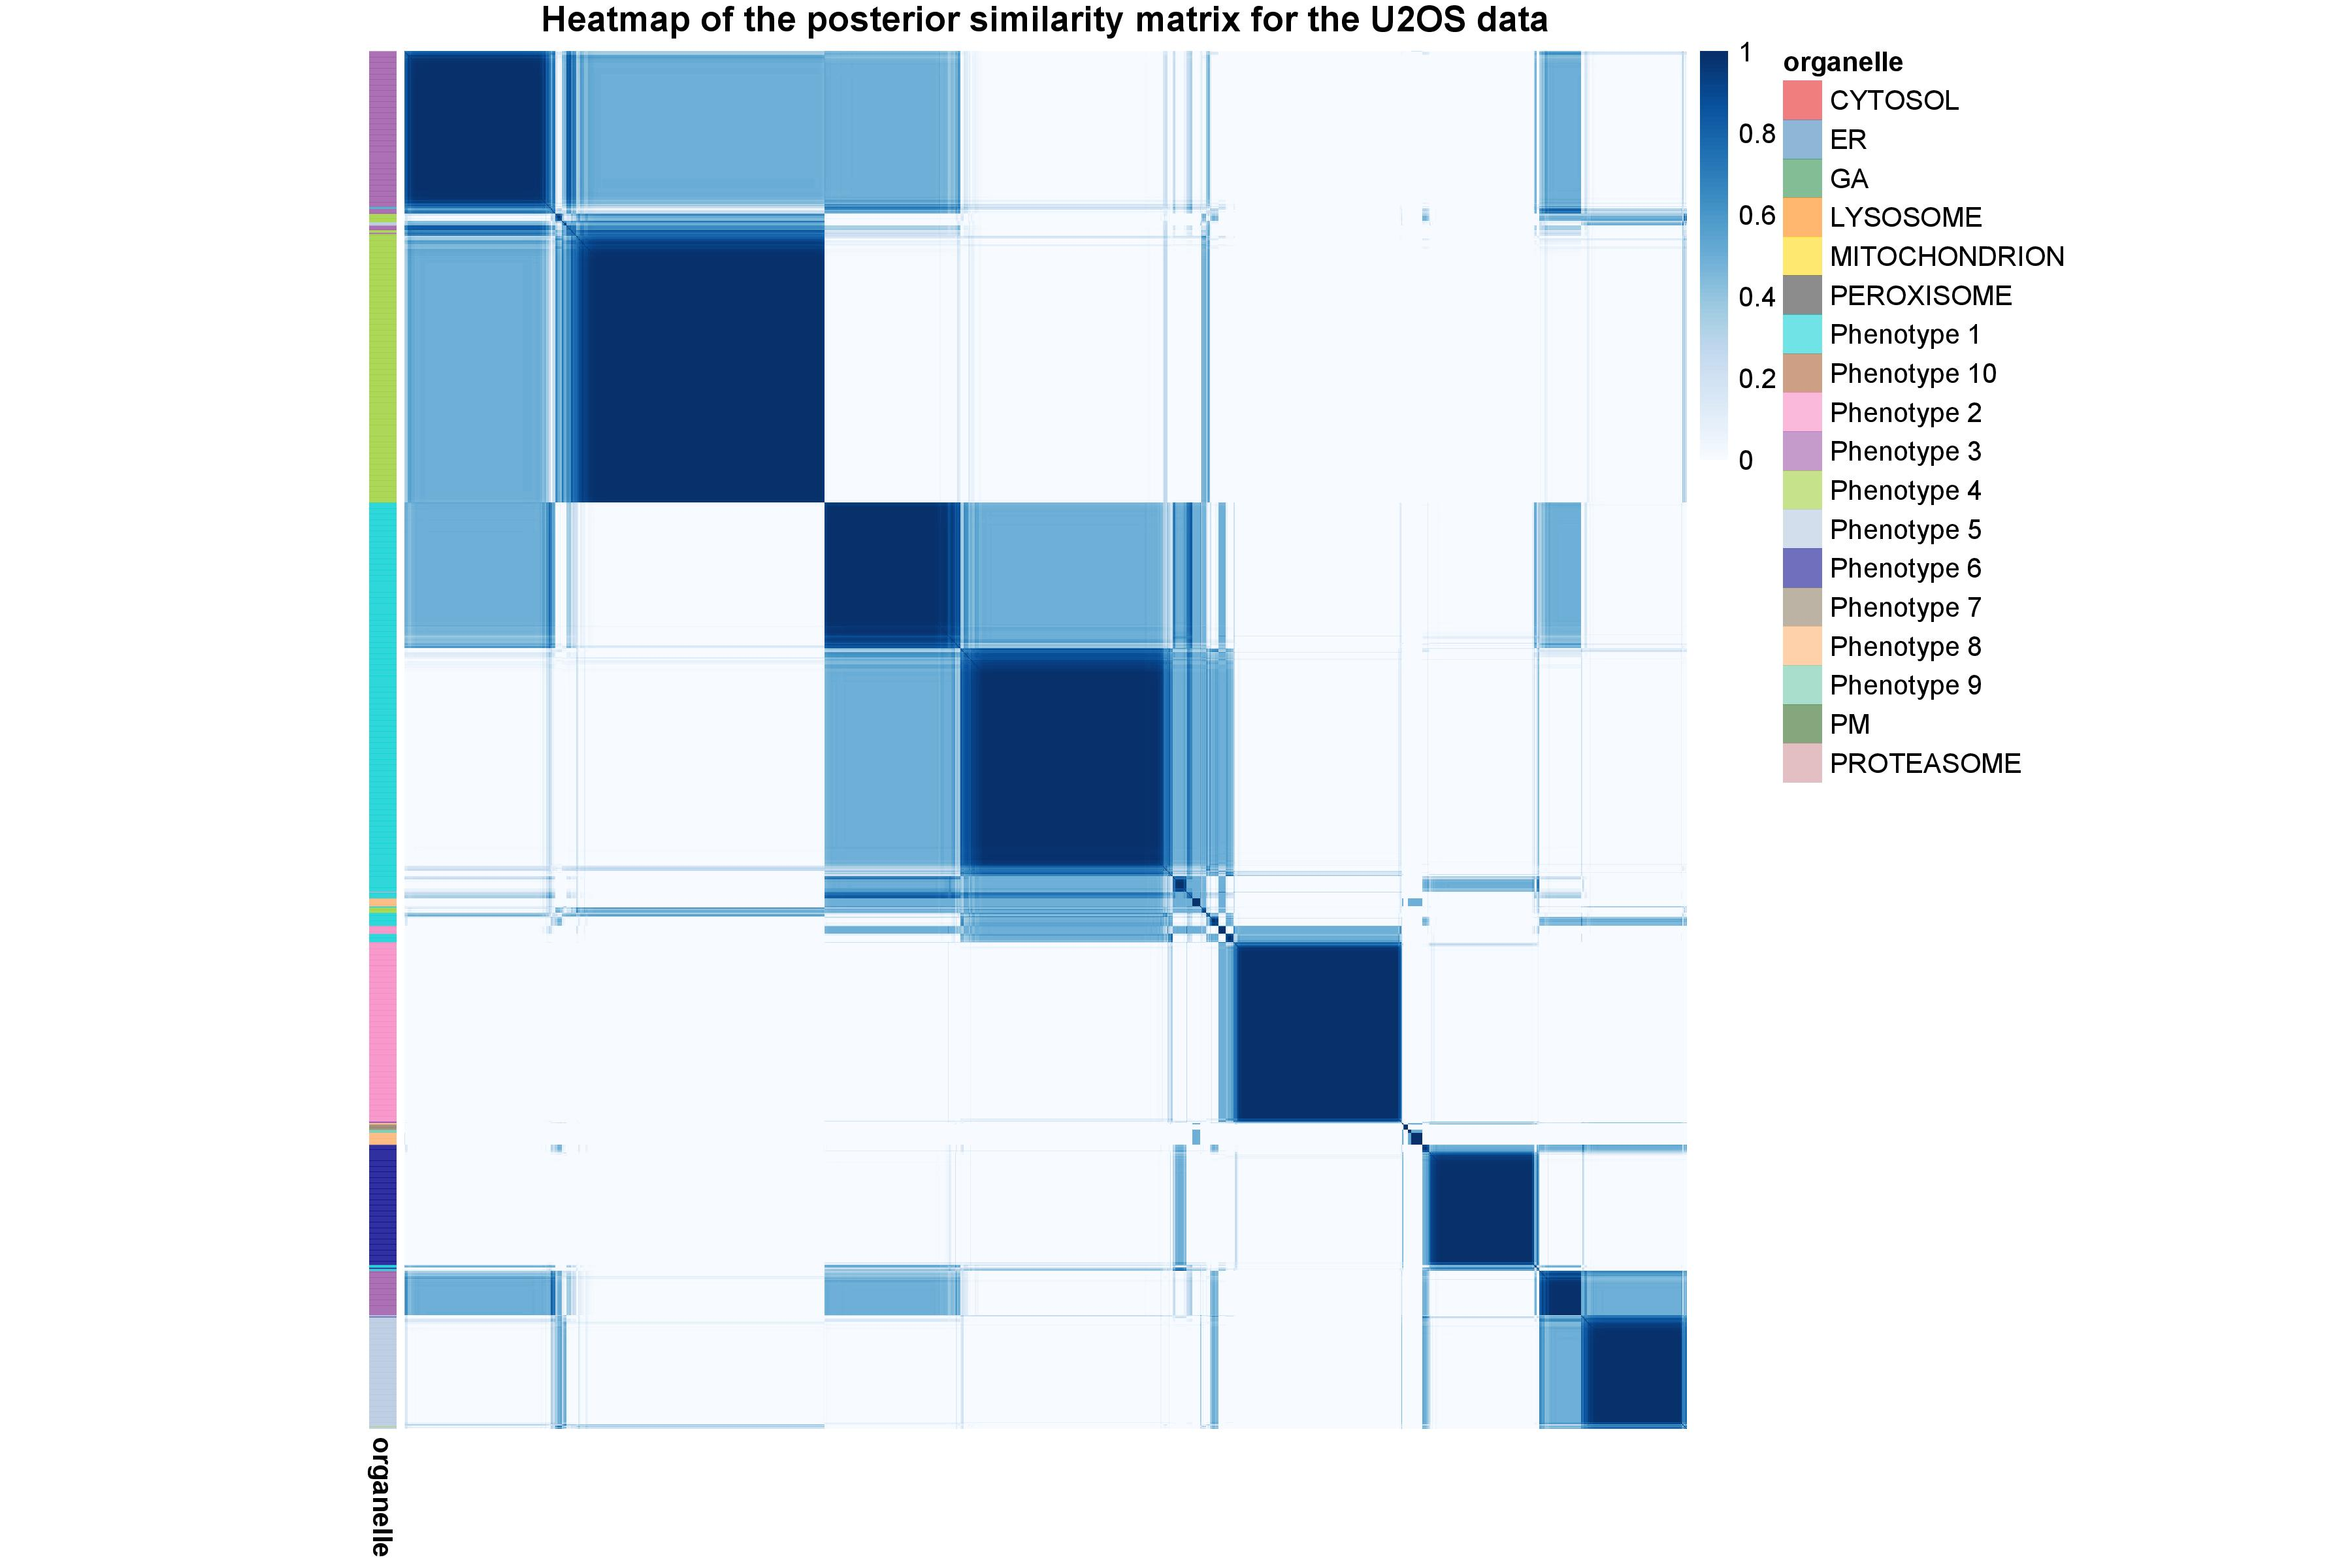
\includegraphics[height=2.5in]{heatmapuU2oshl.jpg}
	\caption{}
\end{subfigure}
	\caption{(a,c) PCA plots of the \textit{hyper}LOPIT mESC data and the \textit{hyper}LOPIT U-2 OS cancer cell line data. The points are coloured according to the organelle or proposed new phenotype and are scaled according to the discovery probability. The PCA plots reveal clear clustering structure in the data and confidently identified new phenotypes. (b,d) Heatmaps of the posterior similarity matrix derived from the mESC data and the U-2 OS cell line data demonstrating the uncertainty in the clustering structure of the data. We have only plotted the proteins which have greater than 0.99 probability of belonging to a new phenotype and probability of being an outlier less than 0.95 ($0.5$ for the U-2 OS dataset to reduce the number of visualised proteins.).}
	\label{figure:mouse}.
\end{figure}
\clearpage
\subsection{Uncovering additional sub-cellular structures}
Having validated the ability of Novelty TAGM to recover known experimental design, as well as uncover additional sub-cellular niches resolved in the data, we turn to apply Novelty TAGM to several additional datasets.

\subsubsection{U-2 OS cell line revisited}
 We first consider the LOPIT-DC dataset on the U-2 OS cell line \citep{DC:2018}. For additional validation of our proposed method we removed the nuclear, proteasomal, and ribosomal annotations. Novelty TAGM reveals $10$ phenotypes with at least 1 protein with a discovery probability of greater than $0.99$ and outlier probability of less than $0.95$. These clusters and the uncertainty associated with them can be visualised in figure \ref{figure:DC}.

 In a similar vein to the analysis performed on the \textit{hyper}LOPIT U-2 OS dataset, we initially use the available HPA data to validate these clusters \citep{Thul:2017}. Phenotypes $3,5,7$ and $9$ display nucleus-associated terms as their most frequent HPA annotation. To obtain additional functional information about these phenotypes, we perform an over-representation analysis on GO Cellular Component terms. Phenotype $3$ reveals both \textit{nucleolus} $(p < 10^{-60})$ and \textit{ribosome} $(p < 10^{-30})$ annotations. Phenotype $5$ reveals a \textit{proteasome} cluster $(p < 10^{-30})$. A chromatin-associated phenotype is also discovered, with phenotype $9$ having terms such as \textit{chromosome} $(p < 10^{-60})$ and \textit{chromatin} $(p < 10^{-40})$ terms significantly over-represented in these clusters. Notably, the first evidence for sub-nuclear resolution in this LOPIT-DC dataset. Phenotype $6$ represents a cluster with mixed annotation with over-representation for both \textit{plasma membrane} $(p < 10^{-8})$ and \textit{extracellular matrix} $(p < 10^{-2})$ and this is supported by HPA annotation with vesicles, cytosol, and plasma membrane being the top three annotations. An extracellular matrix-related phenotype was not previously known in these data and might correspond to exocytic vesicles containing ECM proteins. Furthermore, phenotype $8$ is significantly enriched for \textit{endosomes} $(p < 10^{-55})$, again a novel annotation for this data. In addition, $107$ of the proteins in this phenotype are also localised to the endosome-enriched phenotype presented in the U-2 OS \textit{hyper}LOPIT dataset. Thus, we robustly identify new phenotypes across different spatial proteomics protocols. Hence, we have presented strong evidence for additional annotations in this dataset, beyond the original analysis of the data \citep{DC:2018}; in particular, although a separate chromatin enrichment preparation was not included in the U-2 OS LOPIT-DC analysis and the original authors did not identify sufficient resolution between the nucleus and chromatin clusters in this dataset, Novelty TAGM could, in fact, reveal a chromatin-associated phenotype in the U-2 OS LOPIT-DC data. In addition, we have joint evidence for an endosomal cluster in both the LOPIT-DC and \textit{hyper}LOPIT datasets. Finally, through the discovery probability and by using the PSMs we have quantified uncertainty in these proposed phenotypes, providing rich information for rigorous interrogation of these datasets.
 
 \subsubsection{Saccharomyces cerevisiae}
Novelty TAGM uncovers $8$ phenotypes in the yeast \textit{hyper}LOPIT data with at least $1$ protein with discovery probability greater than $0.95$. Four of these phenotypes have no significant over-represented annotations. The first phenotype is enriched for the \textit{cell periphery} $(p < 10^{-19})$ and \textit{fungal-type vacuole} $(p < 10^{-10})$. Phenotype $3$ has over-represented annotations for the \textit{kinetochore} $(p < 0.01)$, whilst phenotype $4$ is enriched for the \textit{cytoskeleton} $(p < 10^{-7})$. Phenotype $8$ represents a joint Golgi and ER cluster with the COPII-coated ER-to-Golgi transport vesicle enriched in this phenotype $(p < 10^{-14})$, along with the \textit{endoplasmic reticulum membrane} $(p < 10^{-10})$ and the \textit{Golgi membrane} $(p < 10^{-9})$. Indeed, most of the proteins in this phenotype have roles in the early secretory pathway that involve either transport from the ER to the early Golgi apparatus, or retrograde transport from the Golgi to the ER \citep{Bue:2006,Inadome:2005, Otte:2001, Yofe:2016}, also reviewed in \citep{Delic:2013}. The protein Ksh1p (Q8TGJ3) is further suggested through homology with higher organisms to be part of the early secretory pathway \citep{Wendler:2010}. The proteins Scw4p (C7GNF6), Cts1p (C7GVV1) and Scw10p (C7GPV8) \citep{Cappellaro:1998}, as well as Pst1p (C7GT96)\citep{Pardo:2004}, and Cwp1p (C7GVL4) \citep{Yin:2005}, however, are annotated in the literature as localising to the cell wall or extracellular region. It is therefore possible that their predicted co-localisation with secretory pathway proteins observed here represents a snapshot of their trafficking through the secretory pathway. The protein Ssp120p (C7GQY6) is of unknown function and has been show to localises in high throughput studies to the vacuole \citep{Yofe:2016} and to the cytoplasm in a punctate pattern \citep{Huh:2003}. The localisation observed here may suggest that it is therefore either part of the secretory pathway, or traffics through the secretory organelles for secretion or to become a constituent of the cell wall. 
 
\subsubsection{HCMV-infected fibroblast cells} 
We apply Novelty TAGM to the dataset corresponding to the HCMV-infected fibroblast cells 24 hours post infection (hpi) \citep{Jean_Beltran:2016}, and discover $9$ additional phenotypes with at least $1$ protein with discovery probability greater than $0.95$ (demonstrated in figure \ref{figure:DC}). Phenotype $2$ contains a singleton protein and phenotypes $4,6,7,8$ and $9$ are not significantly enriched for any annotations. However, phenotype $3$ is enriched for the \textit{mitochondrial membrane} and  \textit{mitochondrial envelope} annotations $(p < 10^{-4})$; this is an addition to the already annotated mitochondrial class, indicating sub-mitochondrial resolution. Phenotype $1$ is a mixed ribosomal/nuclear cluster with enrichment for \textit{nucleoplasm} $(p < 10^{-5})$ and the \textit{small ribosomal subunit} $(p < 10^{-4})$, which is distinct from phenotype $5$ which is enriched for the \textit{large ribosomal subunit} $(p < 10^{-10})$. This demonstrates unbiased separation of the two ribosomal subunits, which was overlooked in the original analysis \citep{Jean_Beltran:2016}.

\subsubsection{Fibroblast cells without infection} 
Novelty TAGM reveals $7$ phenotypes with at least 1 protein with discovery probability greater than $0.95$ in the control fibroblast dataset. Phenotypes $2,4,5,6$ and $9$ have no significantly enriched Gene Ontology terms (threshold $p = 0.01$). However, we observe that phenotype $3$ is enriched with the \textit{large ribosomal subunit} with significance at level $p < 10^{-7} $. Phenotype $1$ represents a mixed \textit{peroxisome} $(p < 10^{-2})$ and \textit{mitchondrion} cluster $(p < 10 ^{-2})$, an unsurprising results since these organelles possess similar biochemical properties and therefore similar profiles during density gradient centrifugation-based fractionation \citep{DC:2018, Dealtry:1992}. The differing number of confidently identified and biologically relevant phenotypes discovered between the two fibroblast datasets could be down to the differing levels of structure between the two datasets. Indeed, it is evident from figure \ref{figure:Beltran} we see differing levels of clustering structure in these datasets.

\begin{figure}
	\begin{subfigure}[t]{0.5\textwidth}
	\centering
	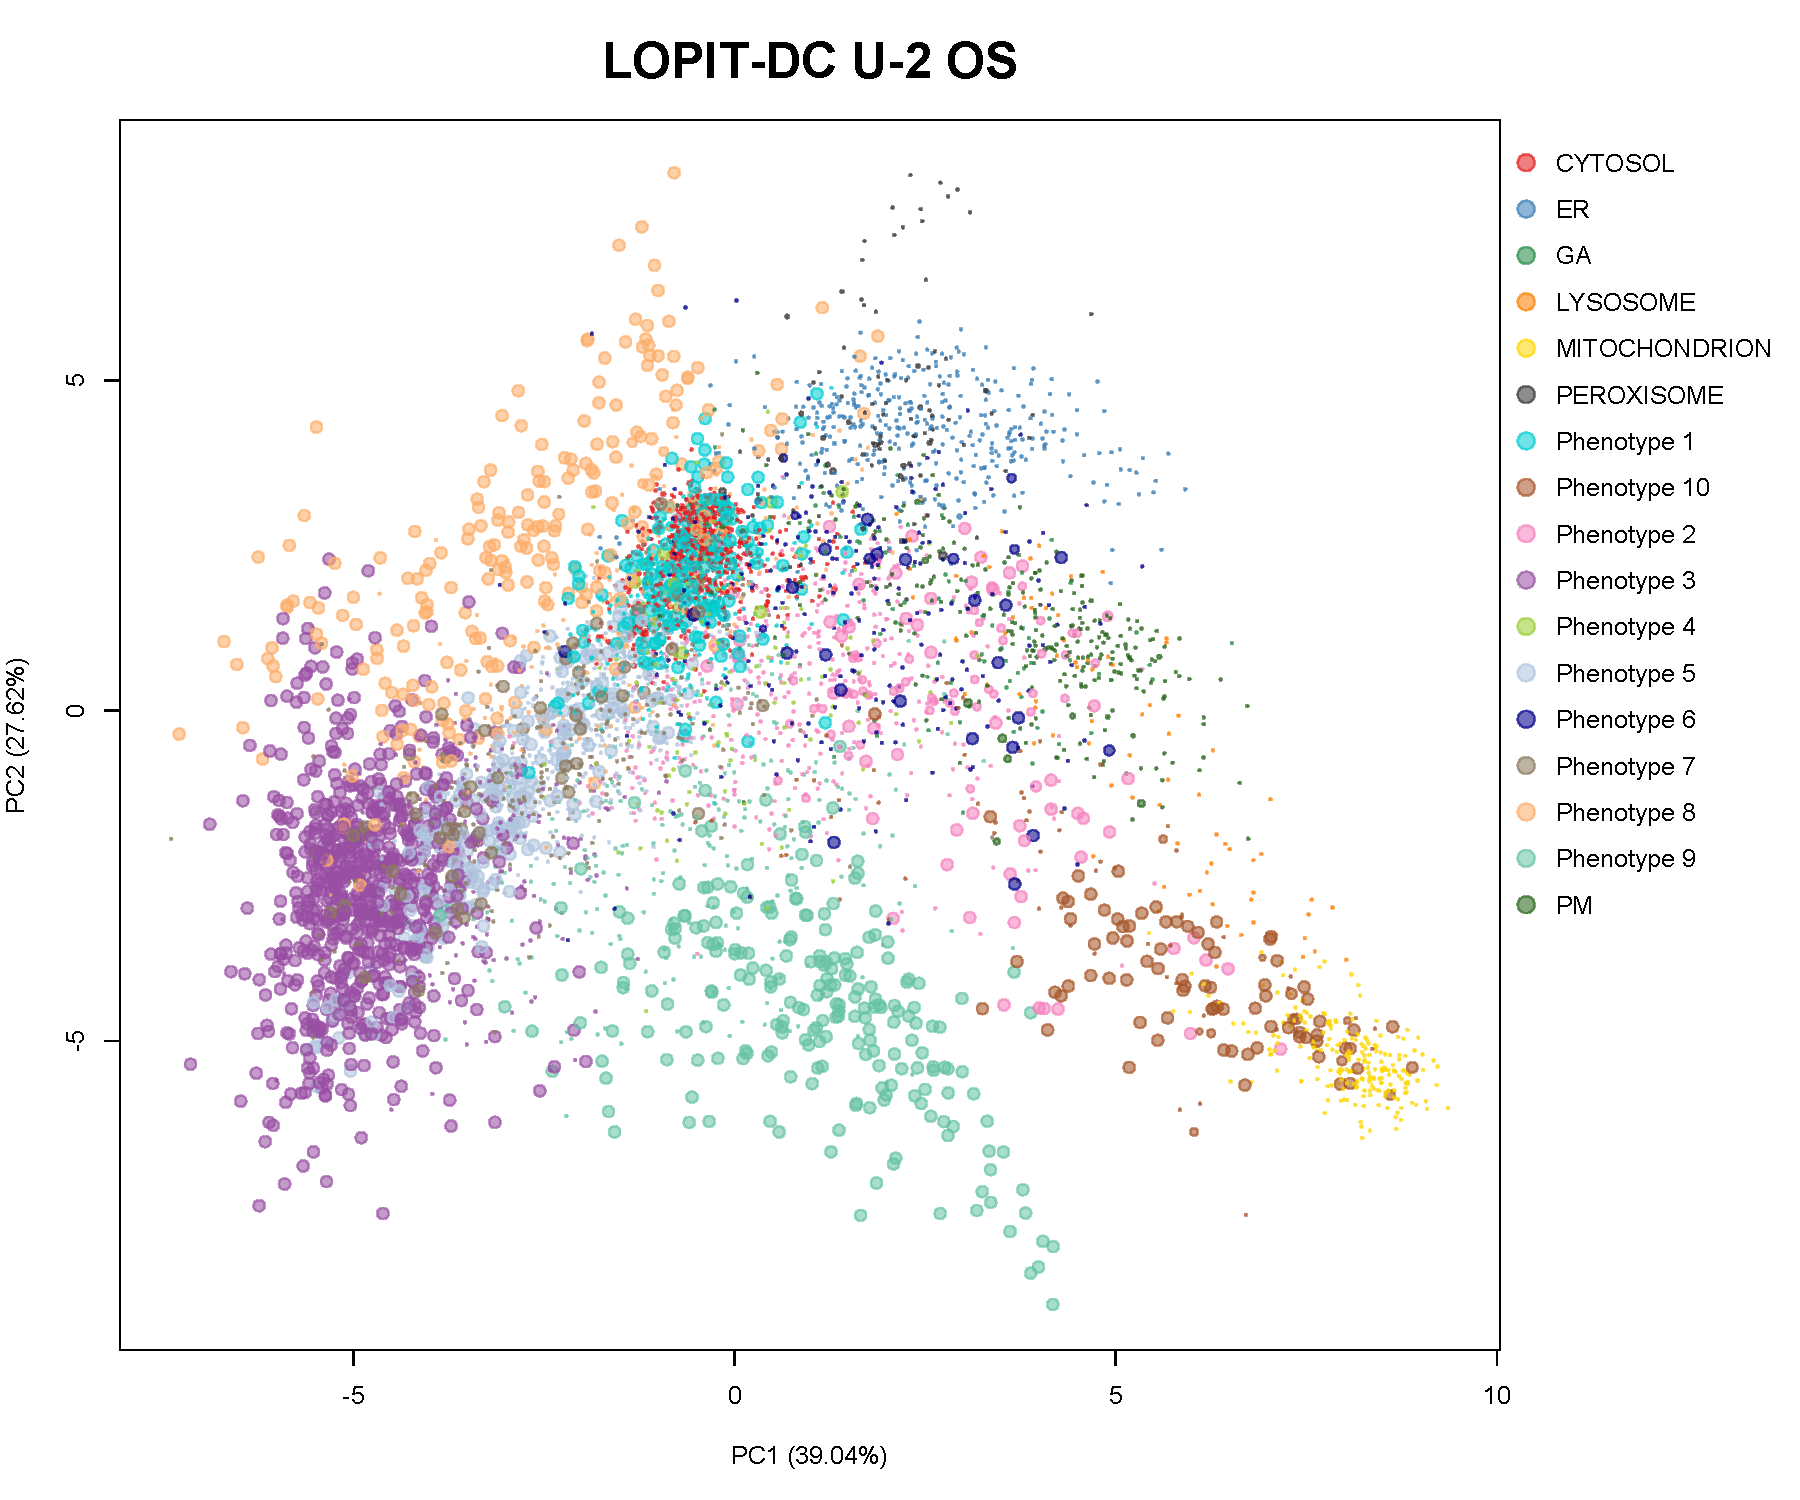
\includegraphics[height=2.5in]{pcau2osdc.pdf}
	\caption{}
\end{subfigure}
\begin{subfigure}[t]{0.5\textwidth}
	\centering
	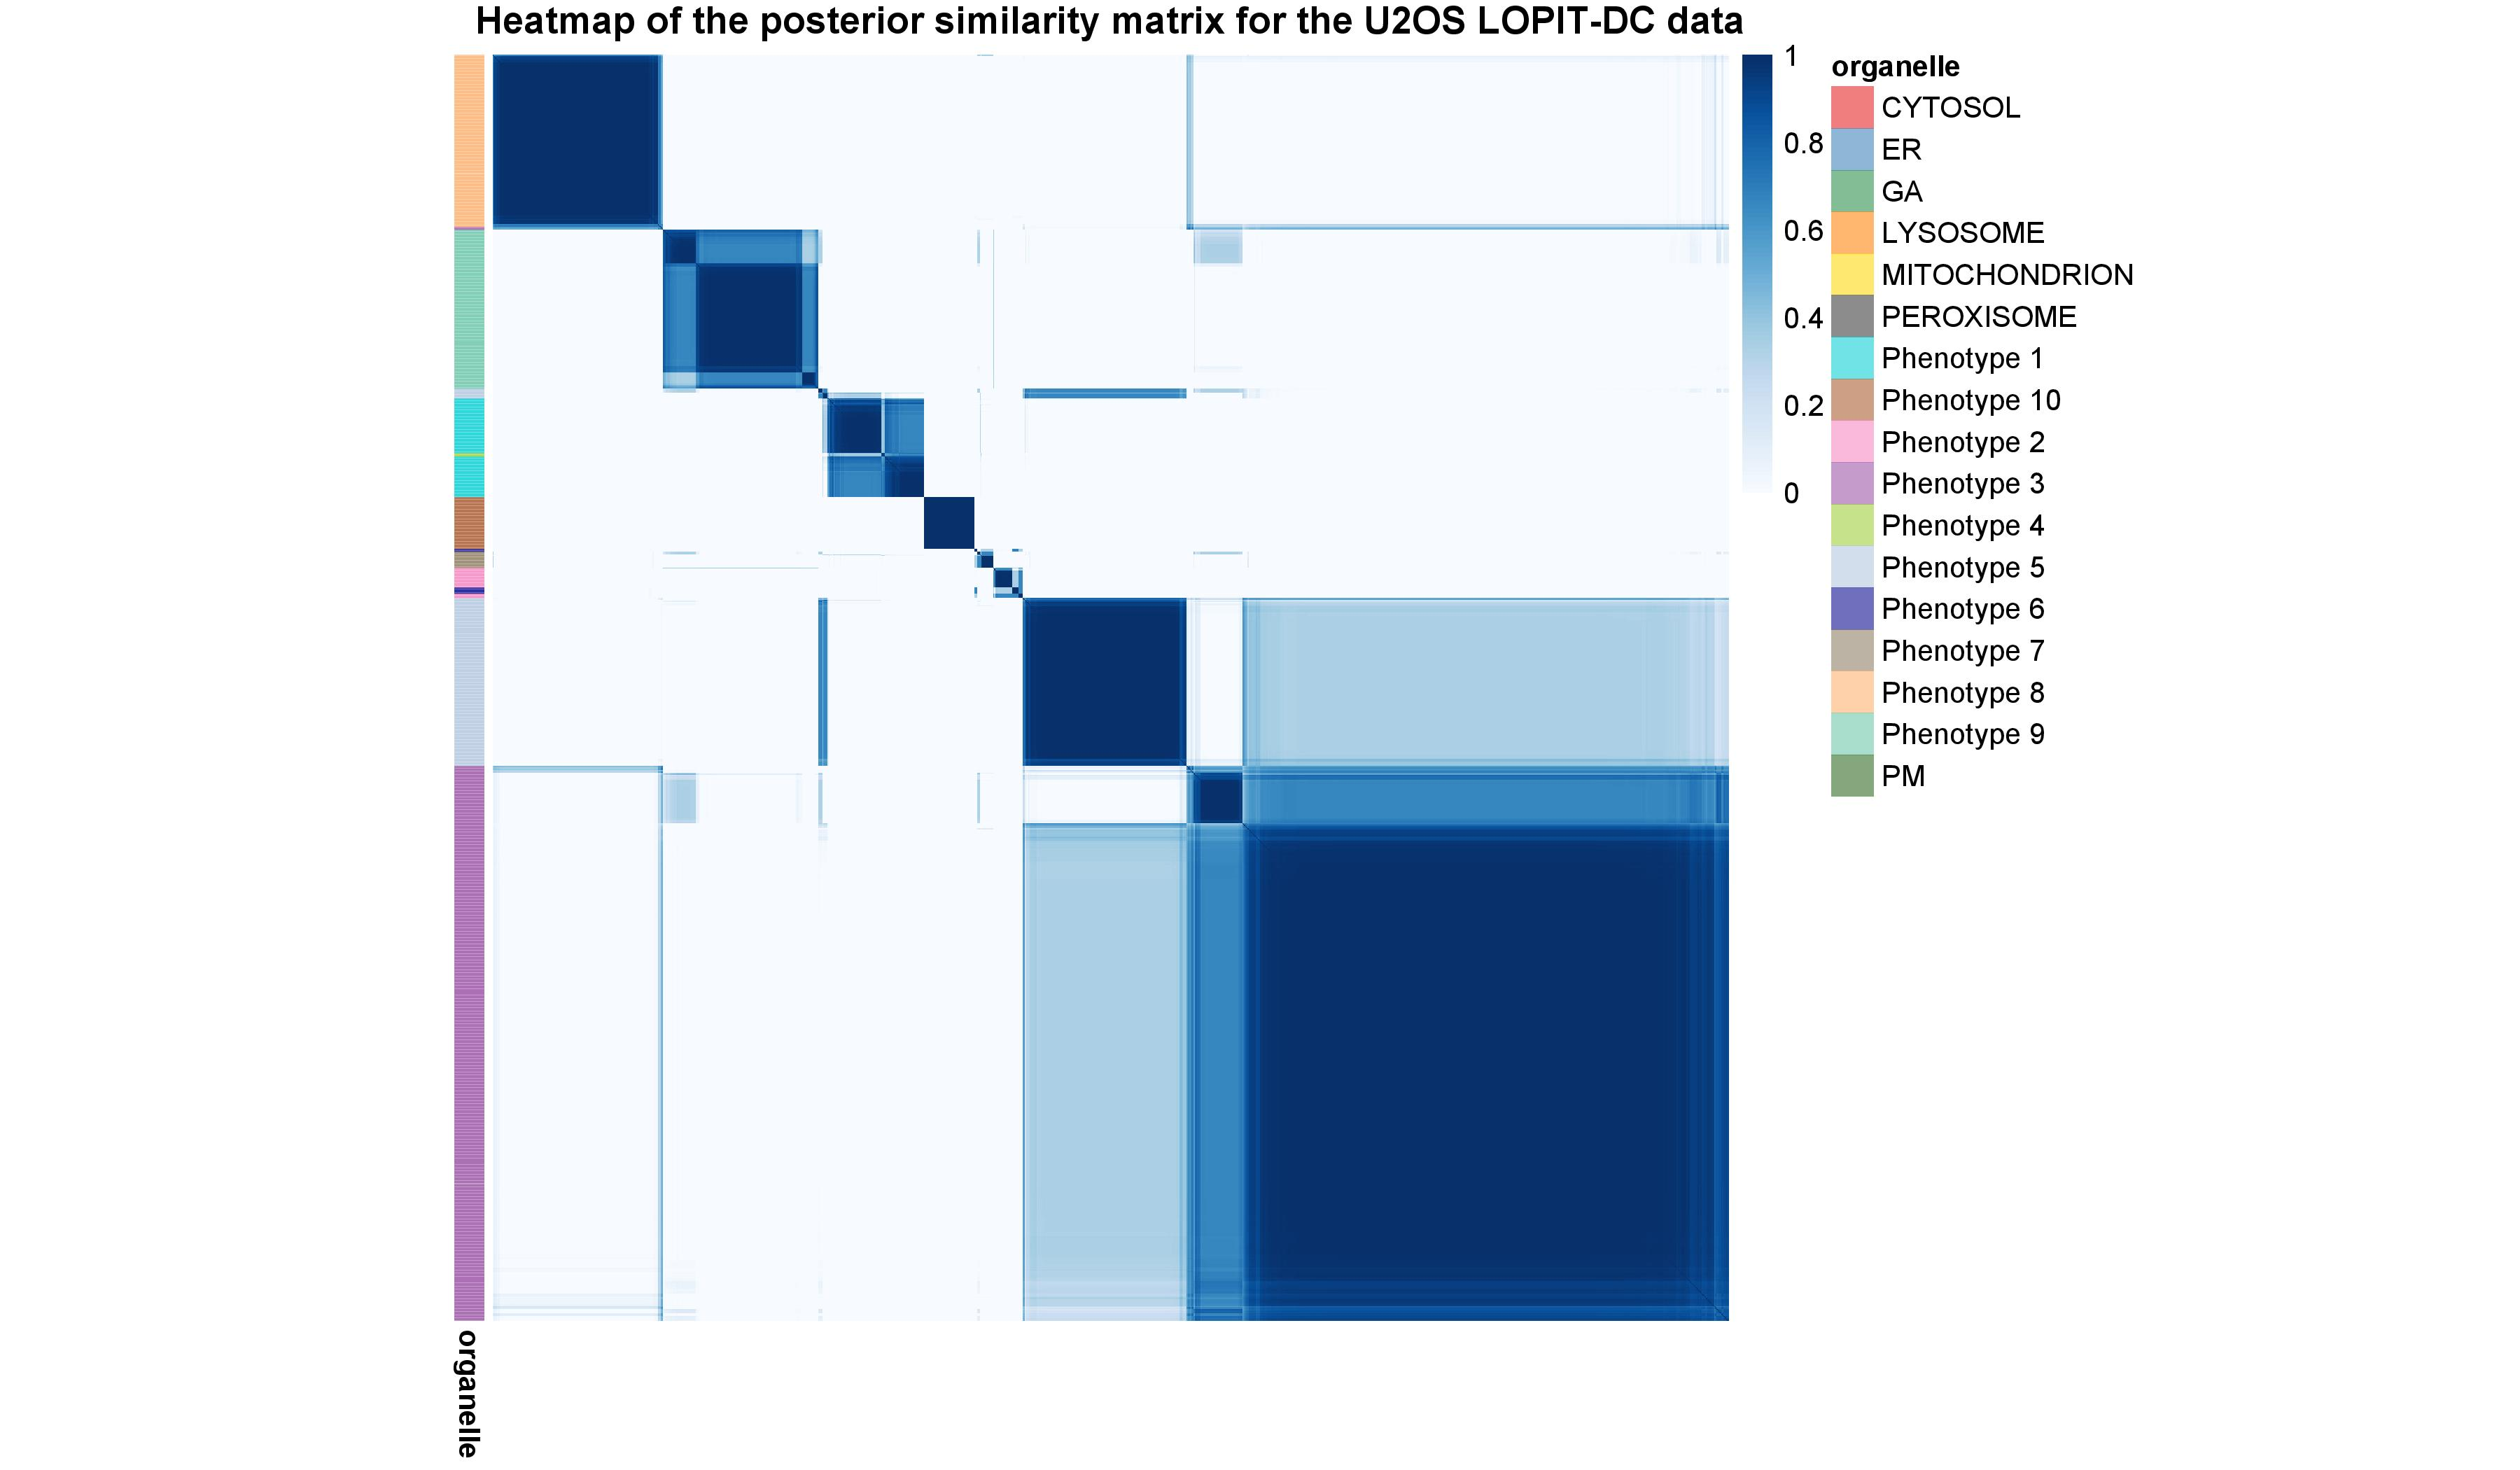
\includegraphics[height=2.5in]{heatmapU2osdc.jpg}
	\caption{}
\end{subfigure}
~
\begin{subfigure}[t]{0.5\textwidth}
	\centering
	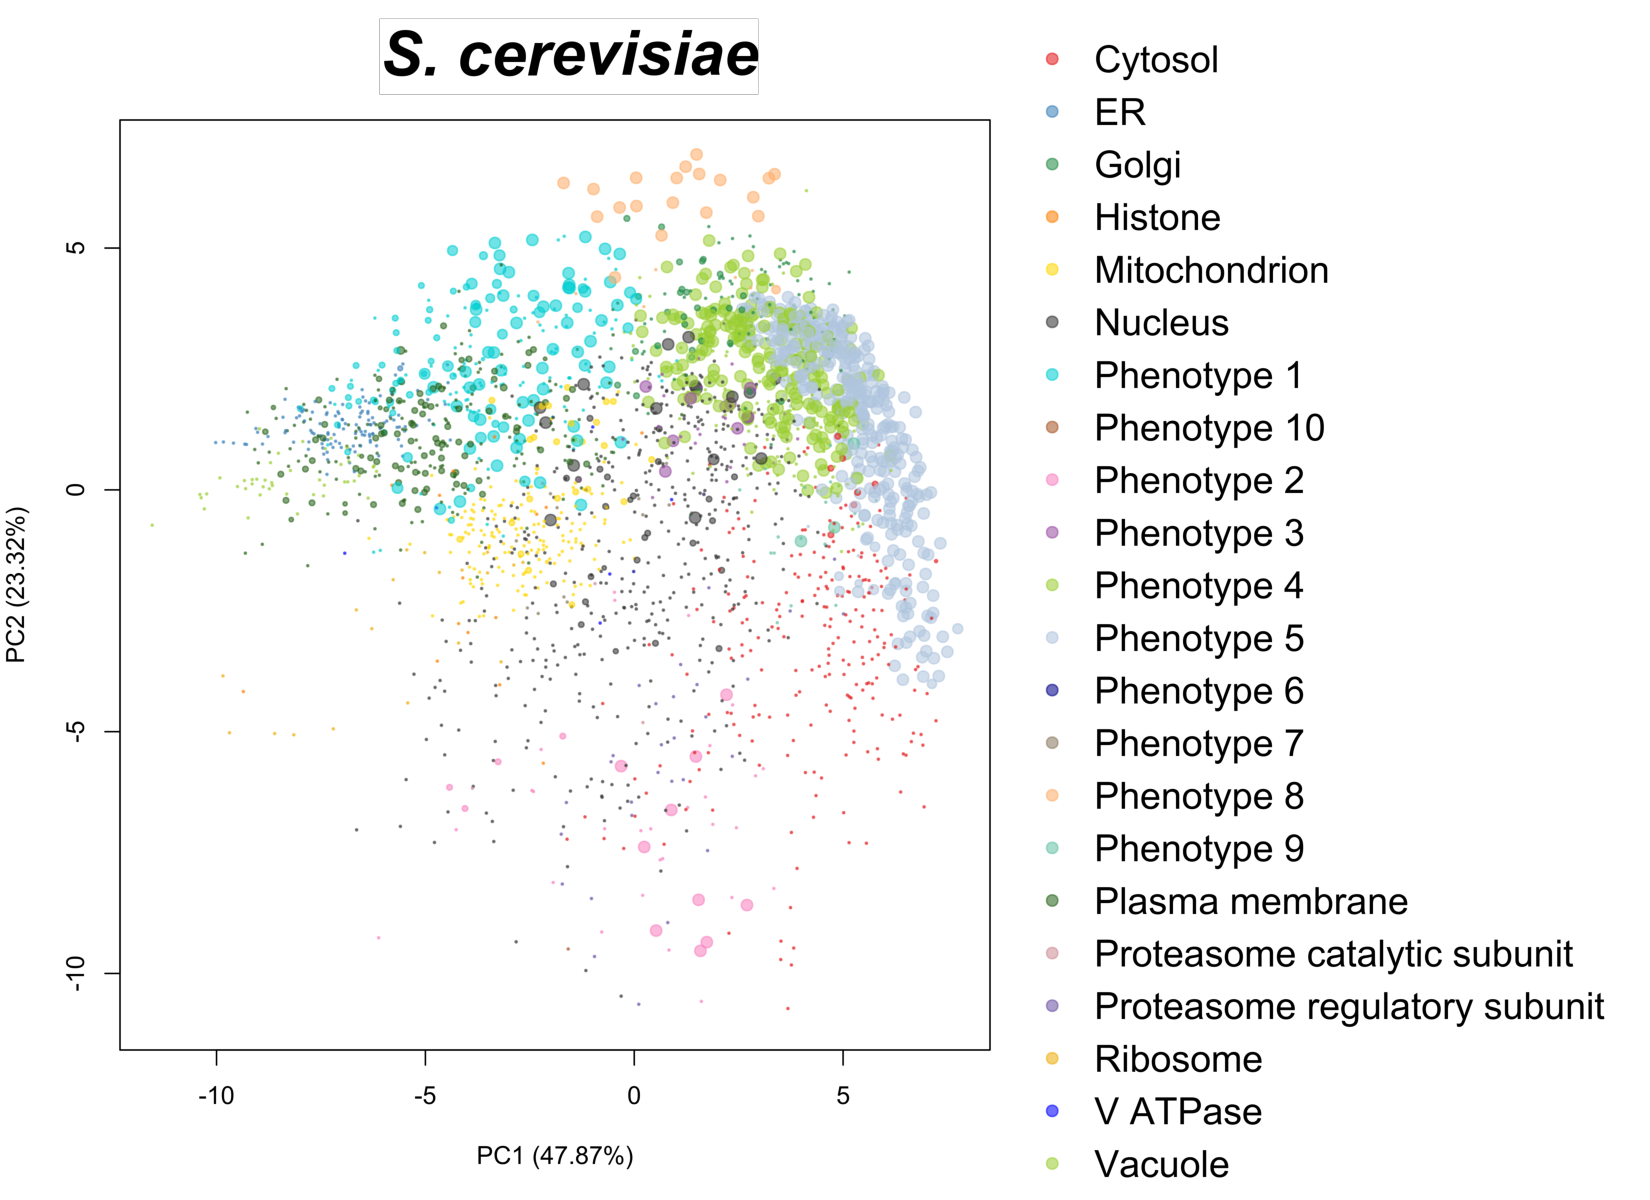
\includegraphics[height=2.5in]{pcaYeast.pdf}
	\caption{}
\end{subfigure}
\begin{subfigure}[t]{0.5\textwidth}
	\centering
	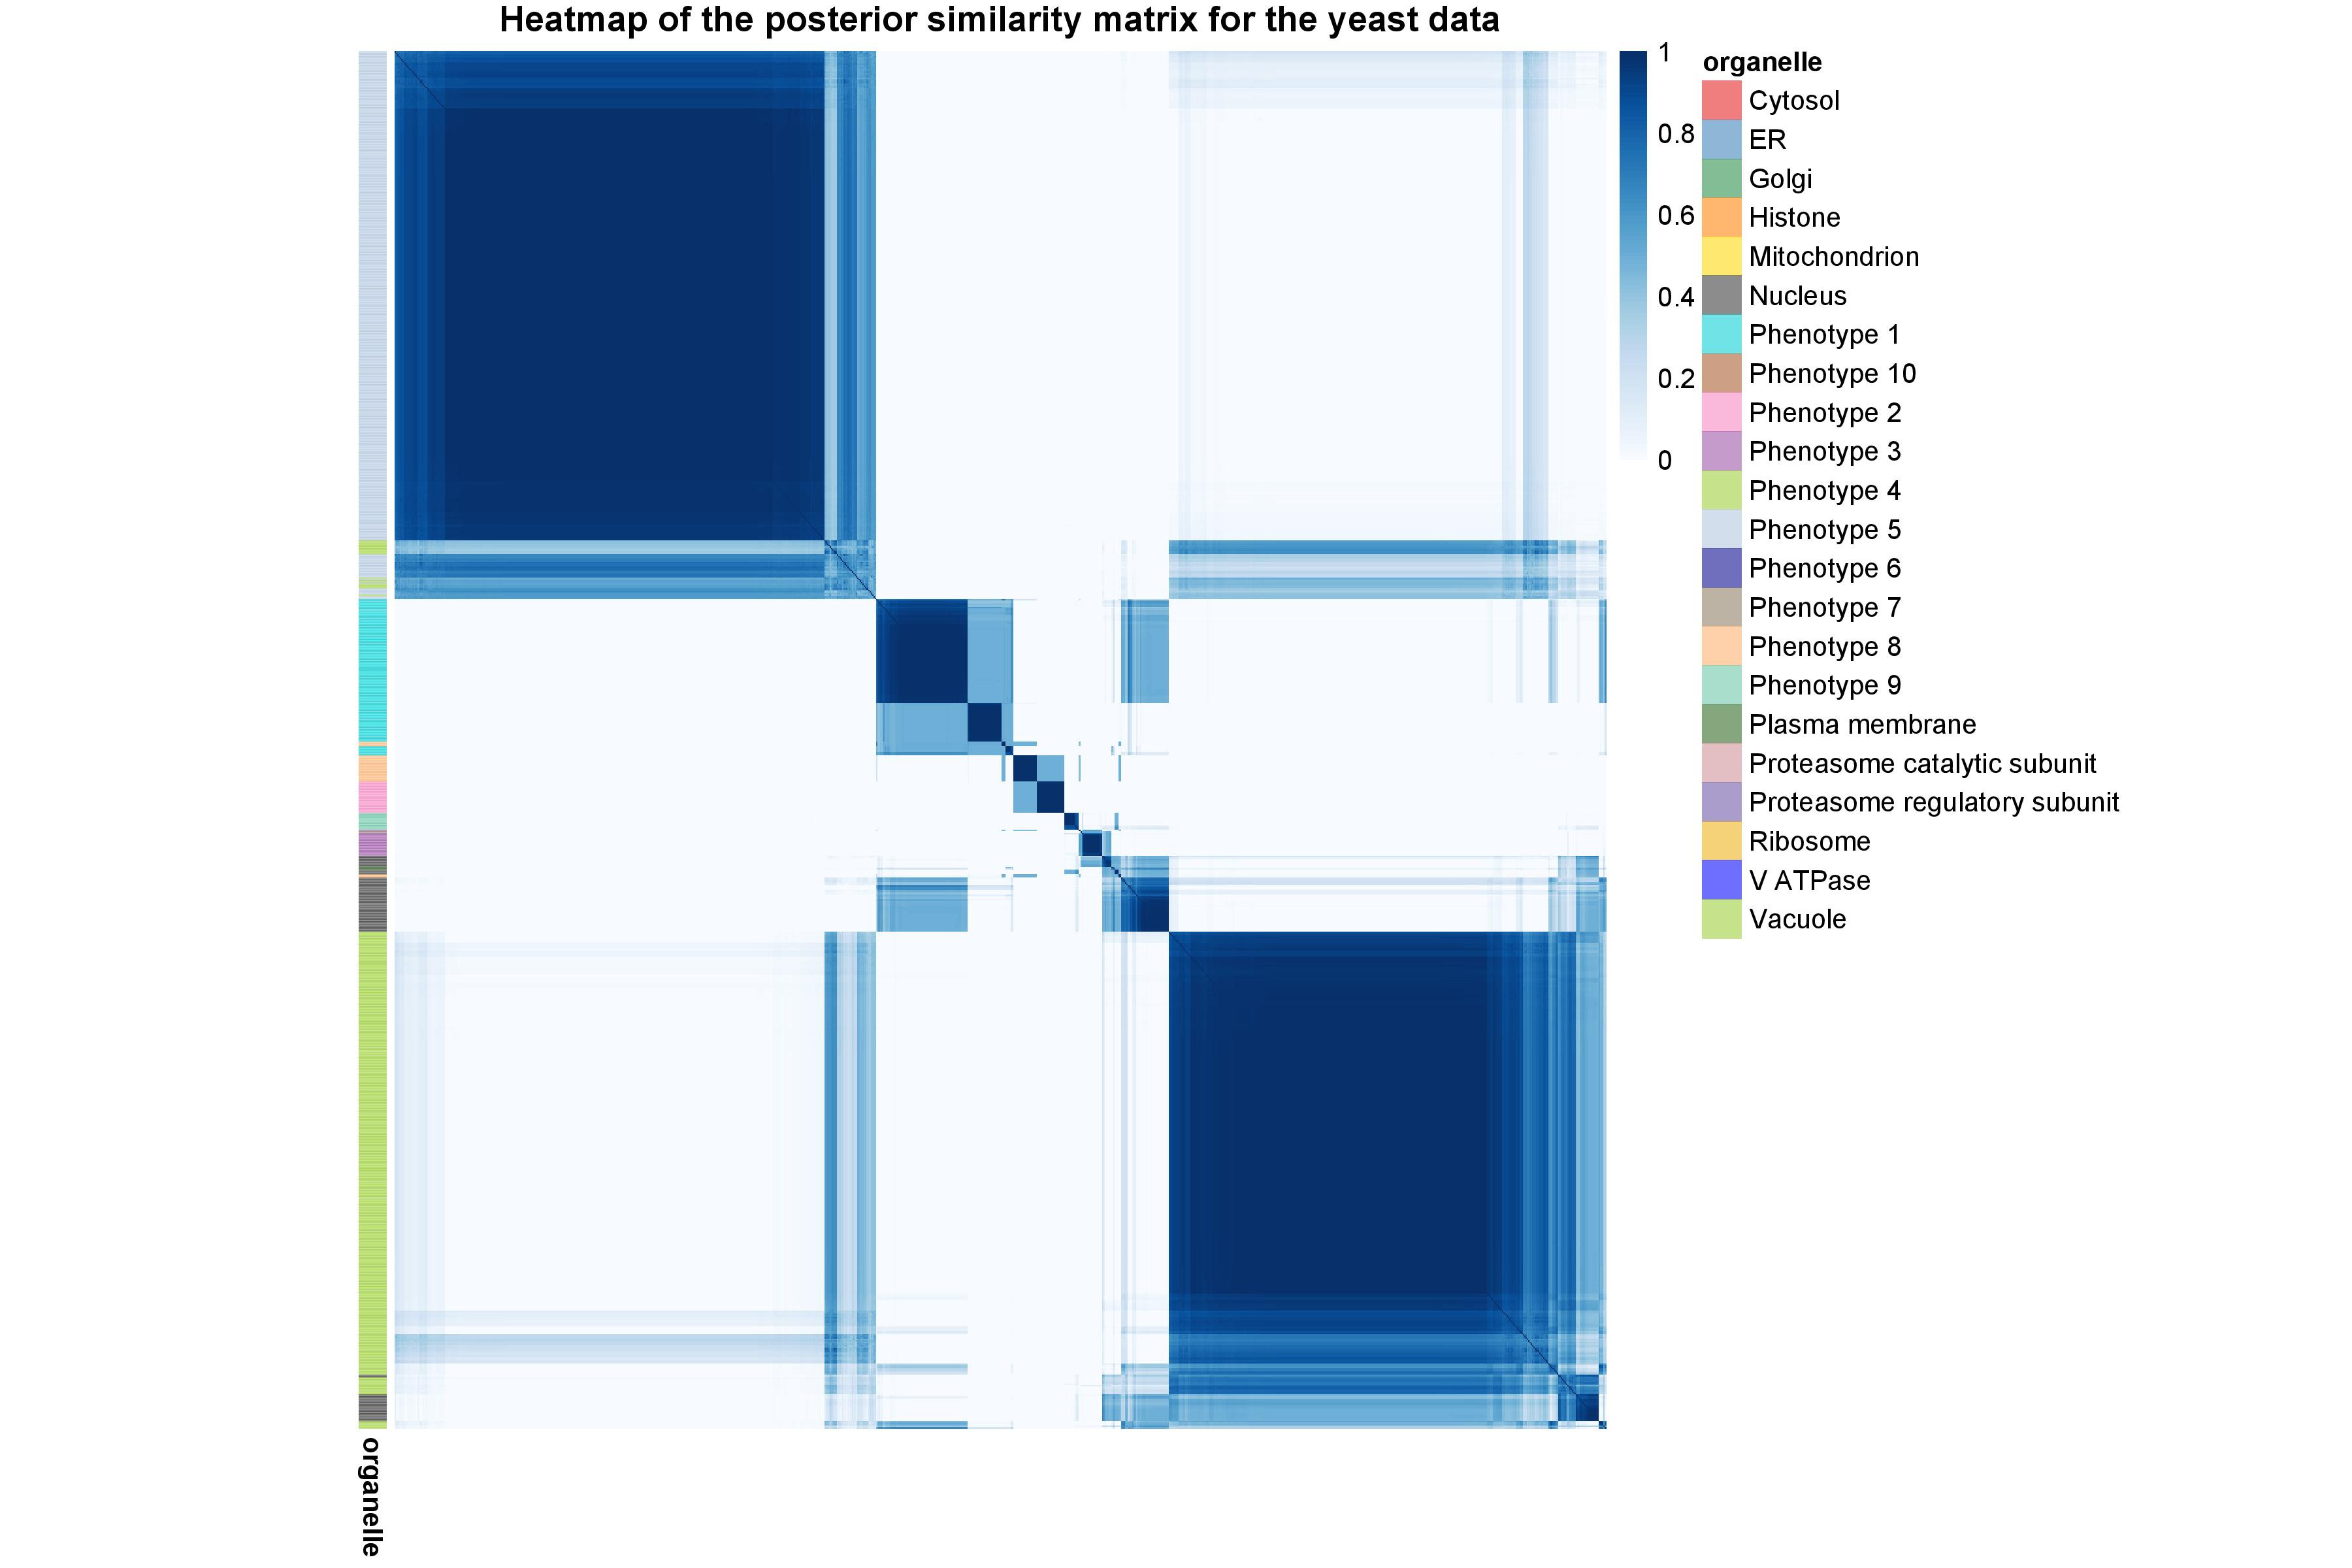
\includegraphics[height=2.5in]{heatmapYeast.jpg}
	\caption{}
\end{subfigure}
\caption{(a, c) PCA plots of the LOPIT-DC U-2 OS data and the \textit{hyper}LOPIT yeast data. The points are coloured according to the organelle or proposed new phenotype and are scaled according to the discovery probability. The PCA plots reveal clear clustering structure in the data and confidently identified new phenotypes. (b,d) Heatmaps of the posterior similarity matrix derived from the U-2 OS and yeast datasets demonstrating the uncertainty in the clustering structure of the data. We have only plotted the proteins which have greater than 0.99 probability of belonging to a new phenotype and probability of being an outlier less than 0.95 ($10^{-5}$ for LOPIT-DC to reduce the number of visualised proteins).}
 \label{figure:DC}
\end{figure}

\begin{figure}
\begin{subfigure}[t]{0.5\textwidth}
	\centering
	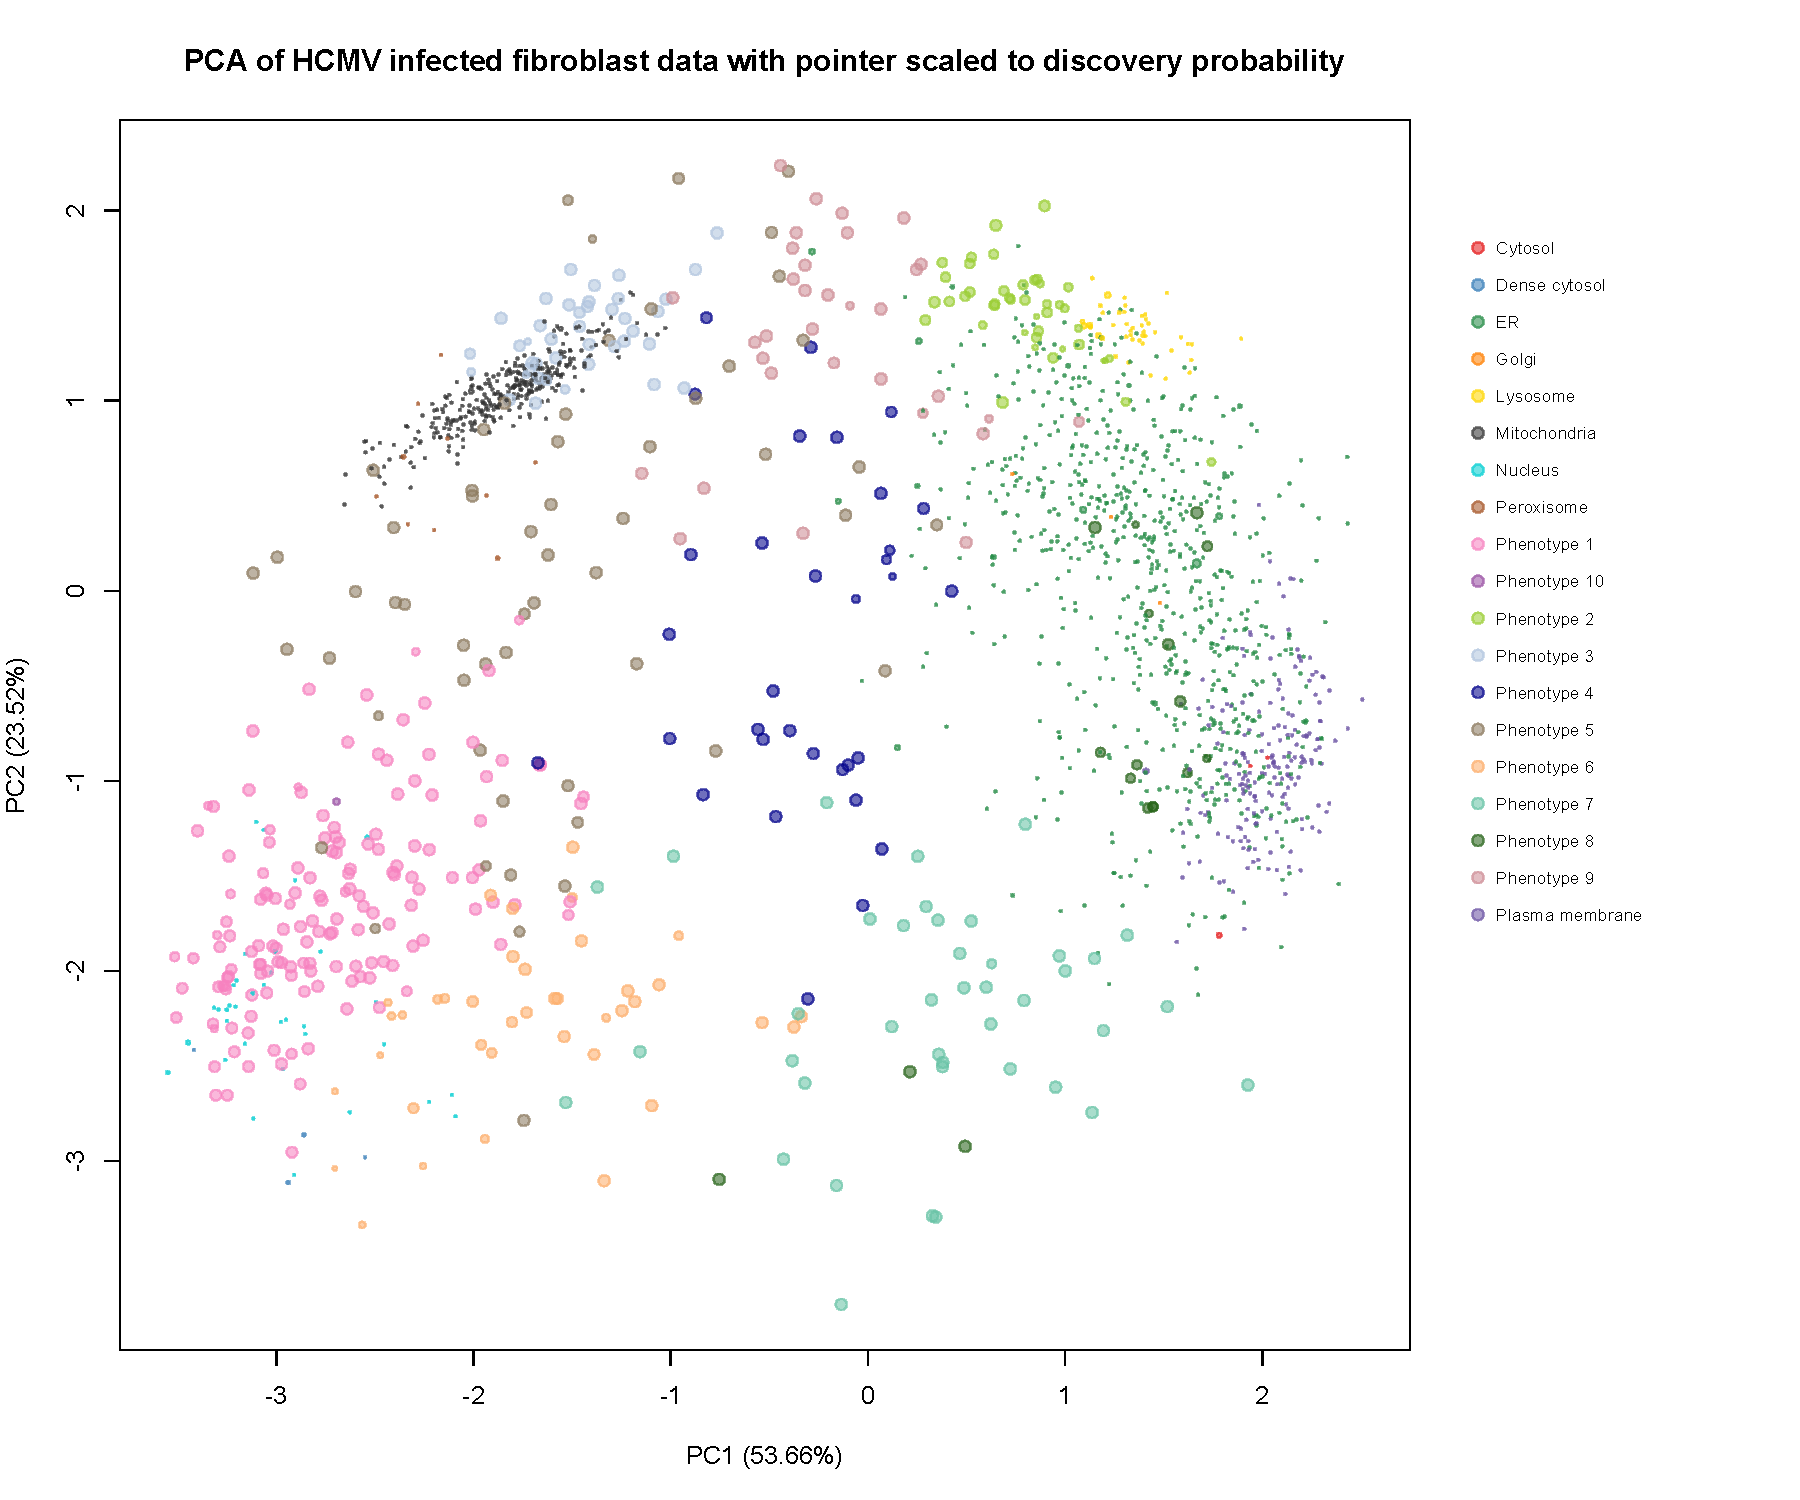
\includegraphics[height=2.5in]{pcaBeltranH.pdf}
	\caption{}
\end{subfigure}	
\begin{subfigure}[t]{0.5\textwidth}
	\centering
	\includegraphics[height=2.5in]{HeatmapHCMV.pdf}
	\caption{}
\end{subfigure}
~
\begin{subfigure}[t]{0.5\textwidth}
	\centering
	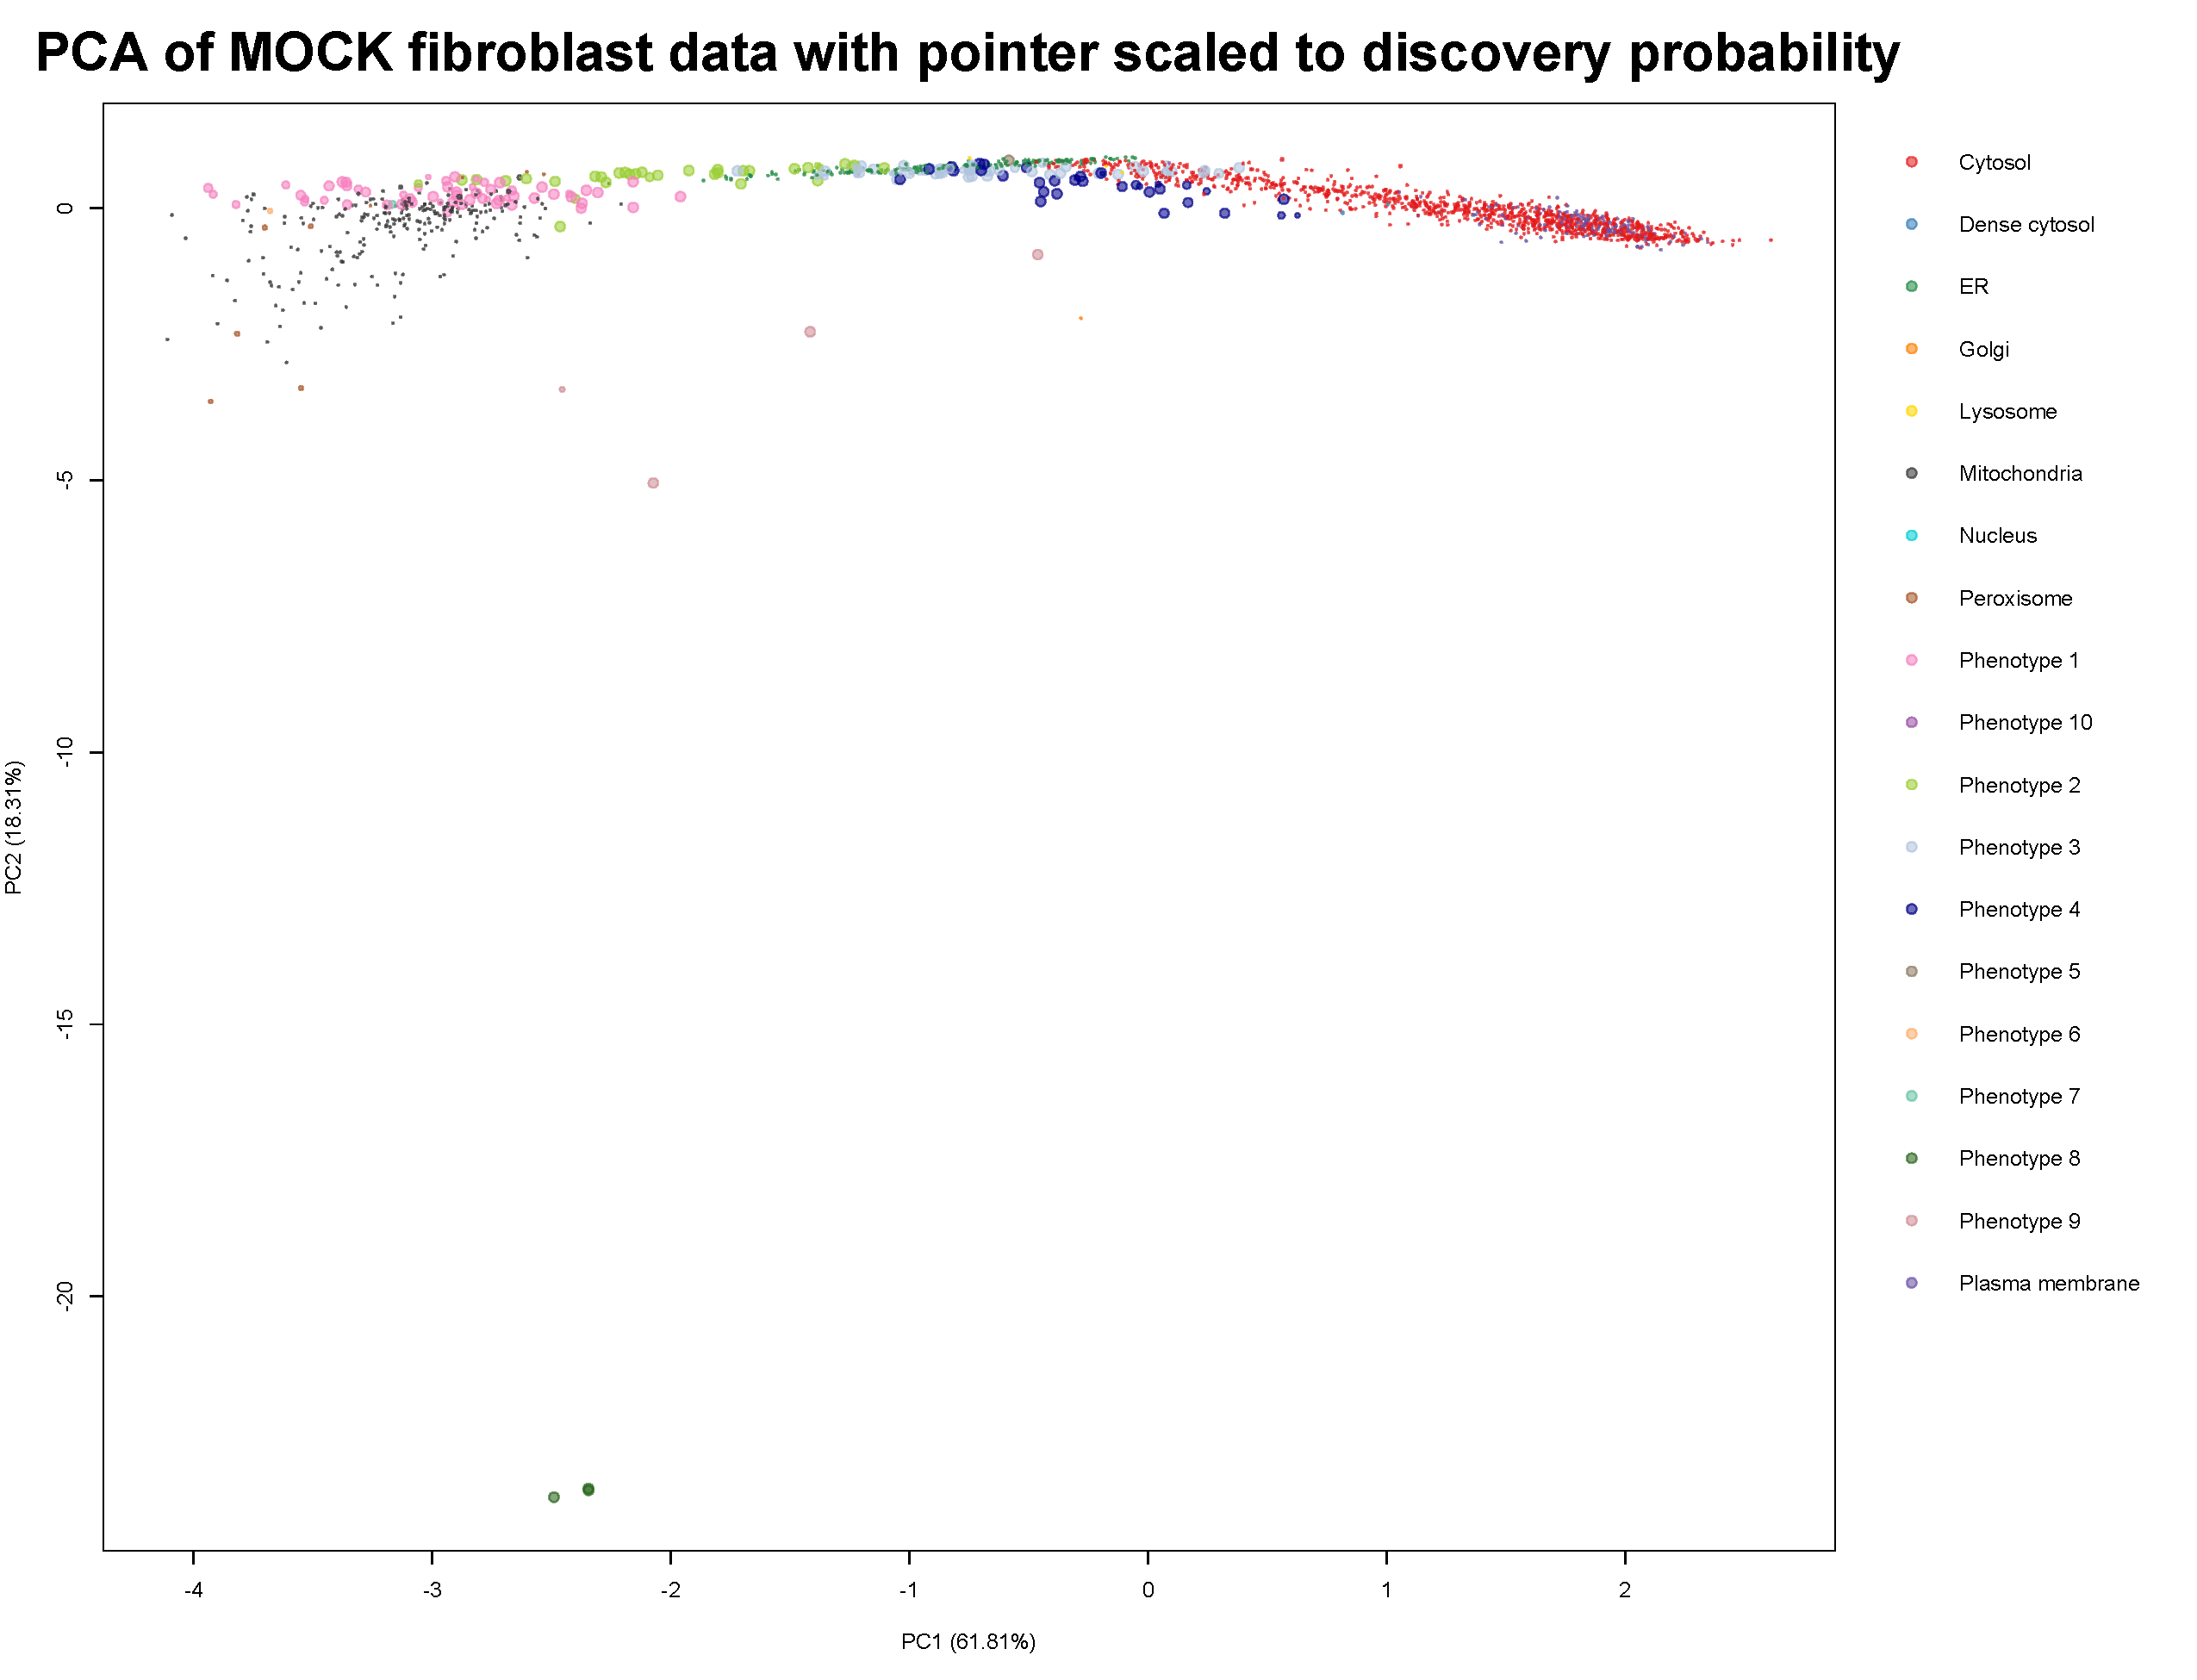
\includegraphics[height=2.5in]{pcaMOCK.pdf}
	\caption{}
\end{subfigure}
\begin{subfigure}[t]{0.5\textwidth}
	\centering
	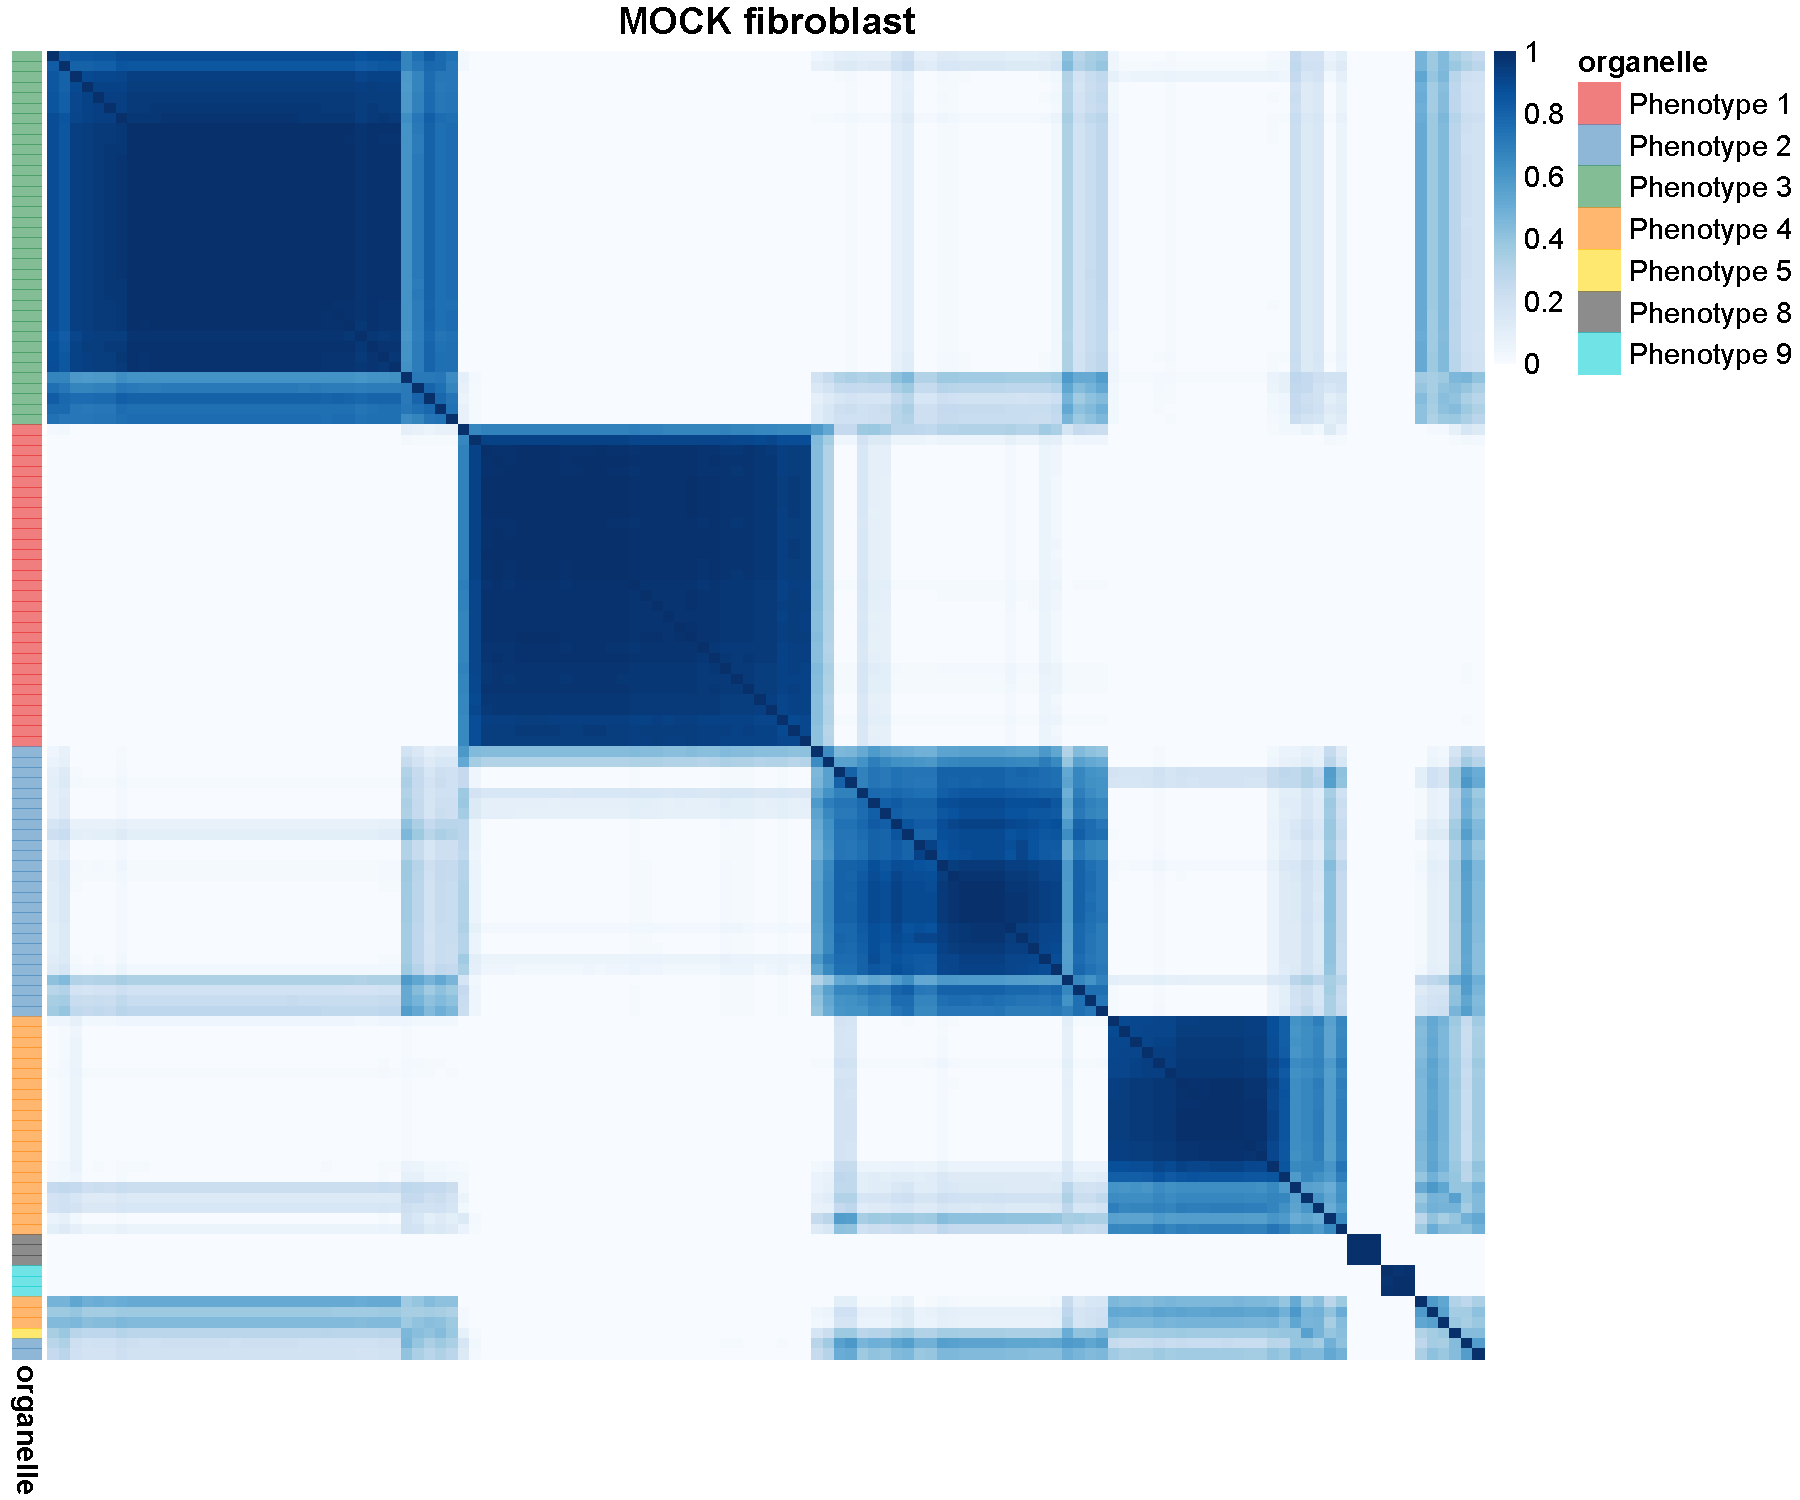
\includegraphics[height=2.5in]{heatmapMOCK.pdf}
	\caption{}
\end{subfigure}
\caption{(a, c) PCA plots of the HCMV-infected fibroblast data 24 hpi and the mock fibroblast data 24 hpi. The points are coloured according to the organelle or proposed new phenotype and are scaled according to the discovery probability. The PCA plots reveal clear clustering structure in the data and confidently identified new phenotypes. (b, d) Heatmaps of the posterior similarity matrix derived from the infected fibroblast data and mock fibroblast data demonstrating the uncertainty in the clustering structure of the data. We have only plotted the proteins which have greater than 0.99 probability of belonging to a new phenotype and probability of being an outlier less than 0.95.}
 \label{figure:Beltran}
\end{figure}
\clearpage
\subsection{Refining annotation in organellar maps}
The Dynamic Organellar Maps (DOM) protocol was developed to reduce the time taken to perform MS-based spatial proteomic mapping, albeit at the cost of organelle resolution \citep{Itzhak:2016,Gatto:2018}. The three datasets analysed here are two HeLa cell line \citep{Itzhak:2016, Hirst:2018} and a mouse primary neuron dataset \citep{Itzhak::2017}. All three of these datasets have been annotated to contain a mixed class called "large protein complexes''. This class contains a mixture of cytosolic, ribosomal, proteasomal and nuclear sub-compartments that pellet during the centrifugation step used to capture this mixed fraction \citep{Itzhak:2016}. We apply Novelty TAGM to these data and remove this "large protein complexes" class, to derive more precise annotations for these datasets. 
\subsubsection{HeLa cells (Itzhak et. al 2016)}
The HeLa dataset of \cite{Itzhak:2016}, which we refer to as HeLa Itzhak, has $3$ additional phenotypes uncovered by Novelty TAGM. The first phenotype is enriched for the \textit{mitochondrial membrane} $(p < 0.01)$, distinct from the already annotated mitochondrial class. Phenotype $2$ represents a mixed cluster with nucleus-, ribosome- and cytosol-related enriched terms, such as \textit{cytosolic ribosome} $(p < 10^{-40})$, \textit{nucleolus} $(p < 10^{-30})$ and \textit{cytosolic part} $(p < 10^{-25})$. The final phenotype is enriched for \textit{chromatin} and \textit{chromosome} $(p < 10^{-10})$, suggesting sub-nuclear resolution. Furthermore, as a result of quantifying uncertainty, we can see that there are potentially more sub-cellular structures in this data (figure \ref{figure:DOM}). However, the uncertainty is too great to support these phenotypes. 
\subsubsection{Mouse primary neurons}
The mouse primary neuron dataset reveals $10$ phenotypes after we apply Novelty TAGM. However, $8$ of these phenotypes have no enriched GO annotations. This is likely a manifestation of the dispersed nature of this dataset, where the variability is generated by technical artefacts rather than biological signal. Despite this, Novelty TAGM is able to detect two relevant phenotypes: the first phenotype is enriched for \textit{nucleolus} $(p < 0.01)$; the second for \textit{chromosome} $(p < 0.01)$. This suggests additional annotations for this dataset.
\subsubsection{HeLa cells (Hirst et. al 2018)}
The HeLa dataset of \cite{Hirst:2018}, which we refer to as HeLa Hirst, reveals $7$ phenotypes with at least 1 protein with discovery probability greater than $0.95$. However, three of these phenotypes represent singleton proteins. Phenotype $1$ reveals mixed cytosol/ribosomal annotations with the terms \textit{cytosolic ribosome} $(p < 10^{-30})$ and \textit{cytosolic part} $(p < 10^{-25})$ significantly over-represented. There are no further phenotypes with enriched annotations $(\text{threshold } p = 0.01)$, except phenotype $2$ which represents a a mixed extracellular structure/cytosol cluster. For example, the terms \textit{extracellular organelle} $(p <10^{-13})$ and \textit{cytosol} $(p < 10^{-10})$ are over-represented.


\begin{figure}
	\begin{subfigure}[t]{0.5\textwidth}
		\centering
		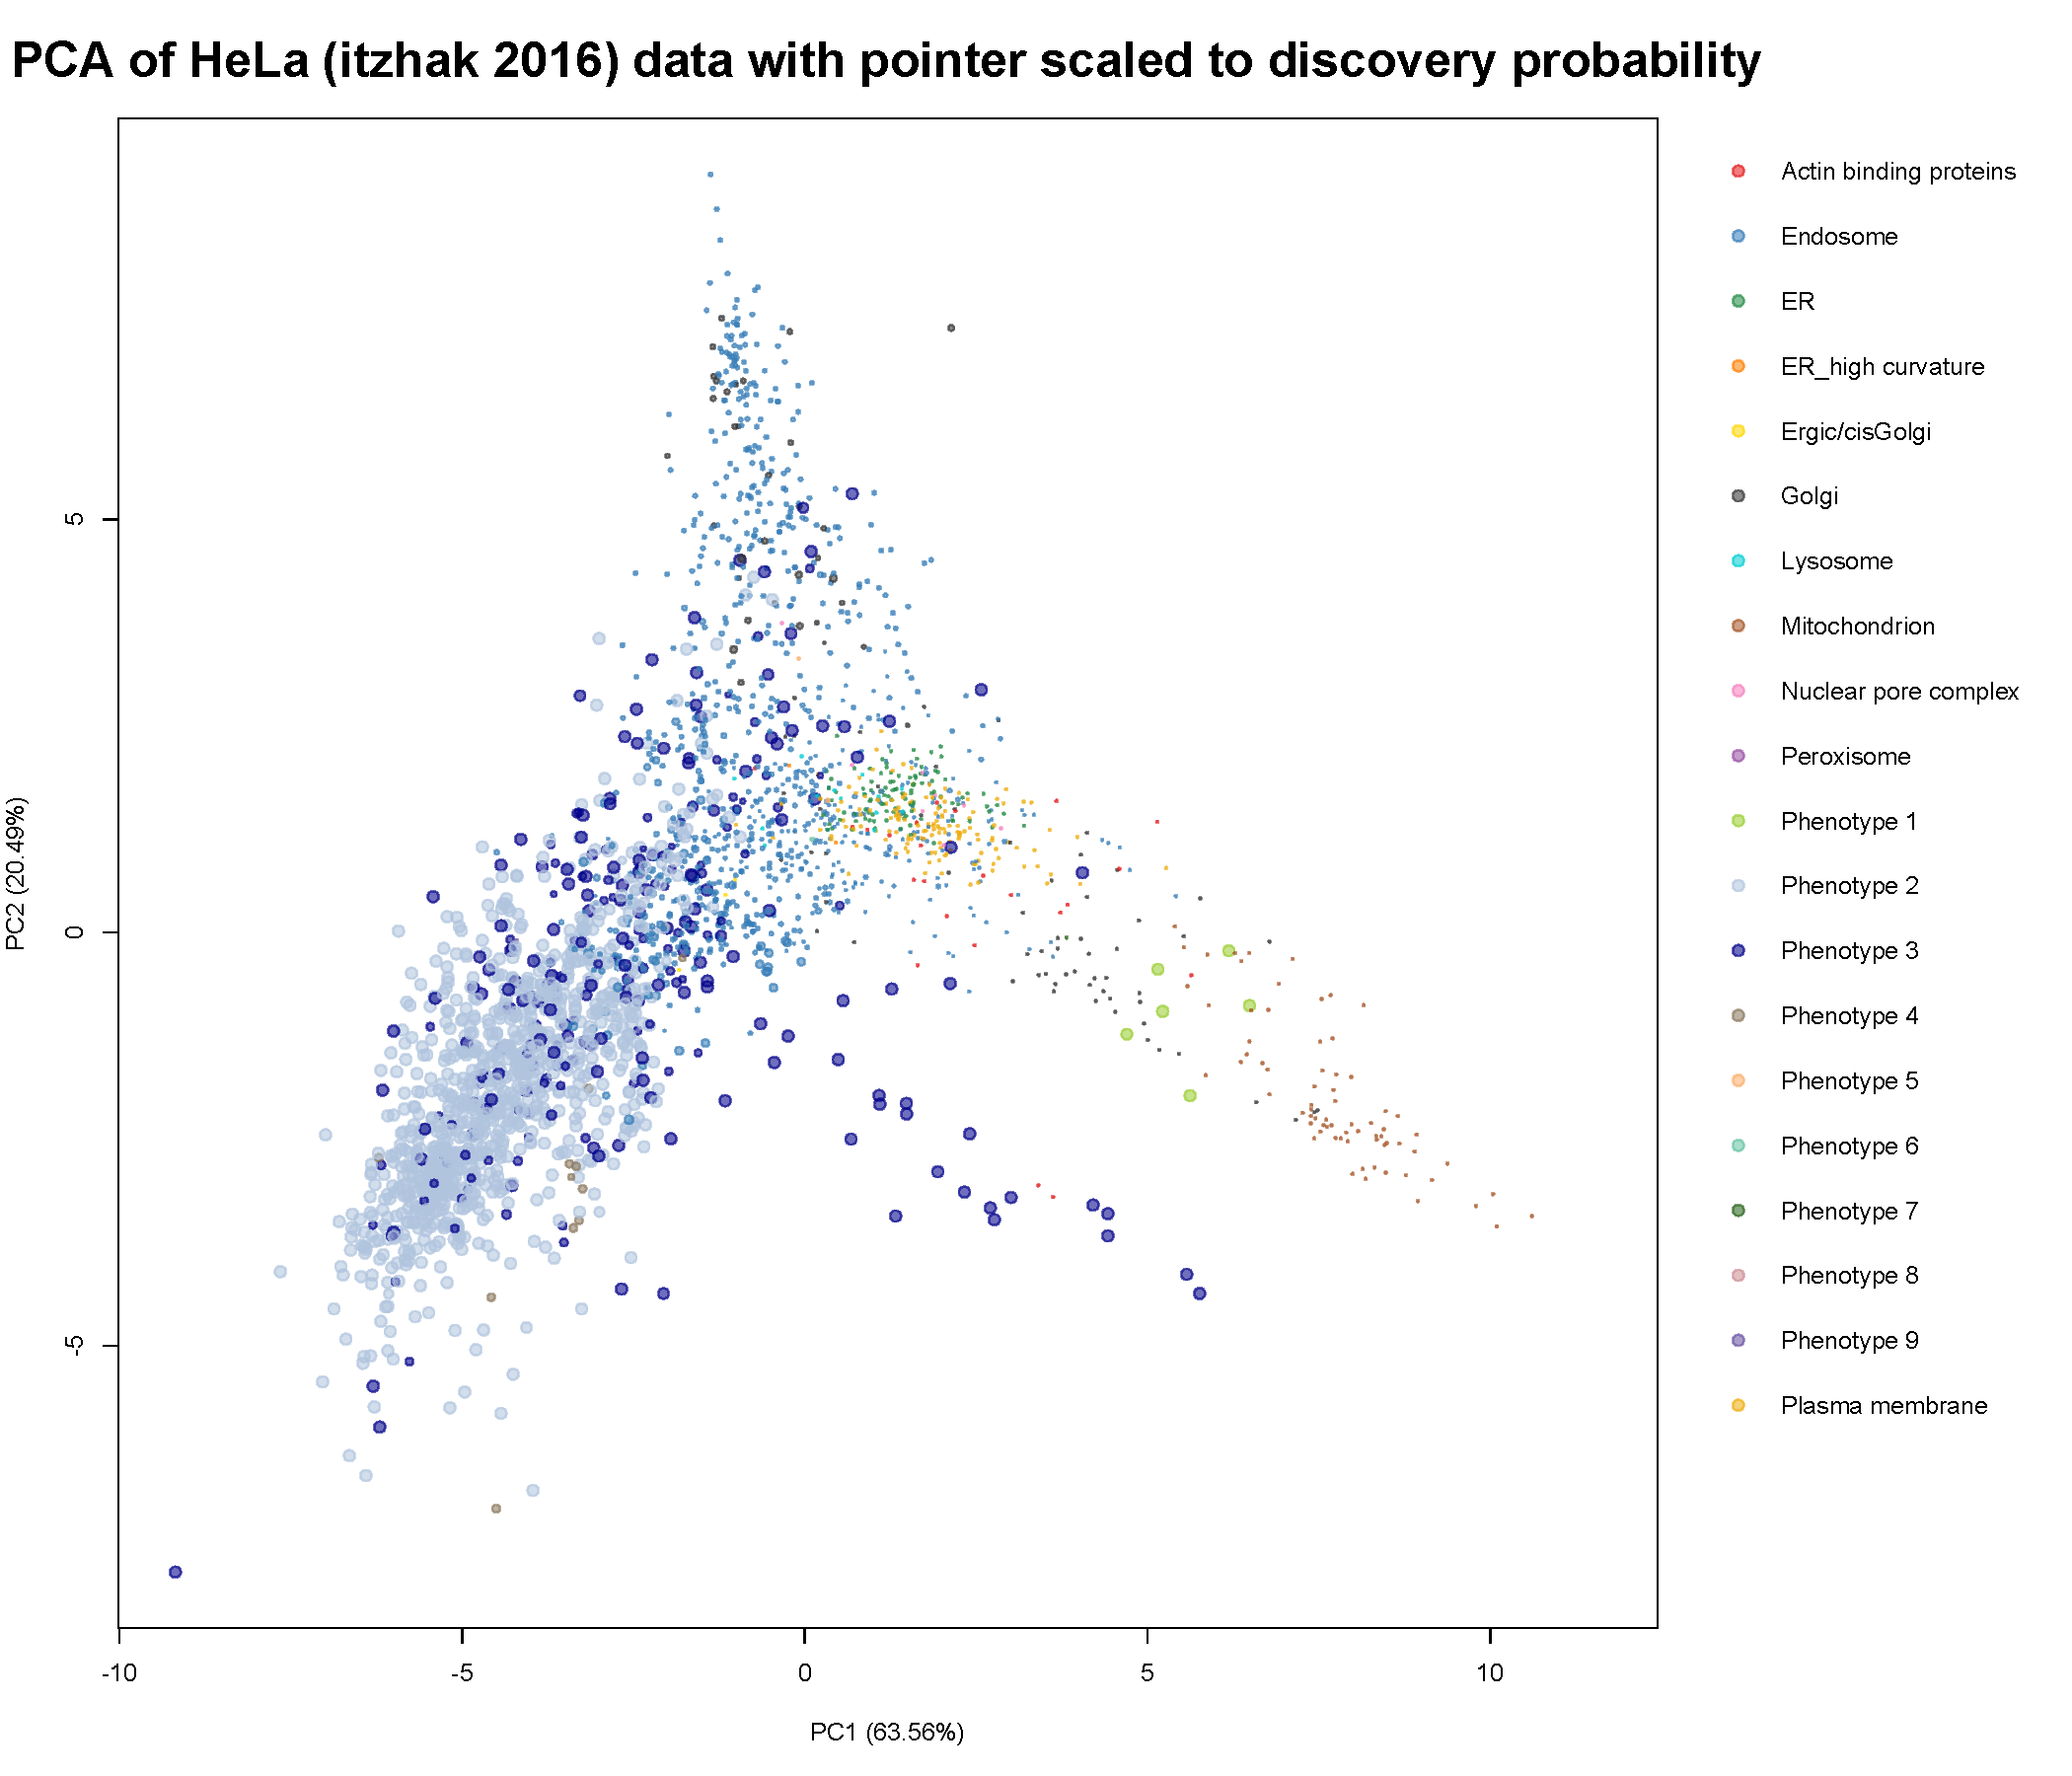
\includegraphics[height=2in]{pcaItzhak2016.pdf}
		\caption{}
	\end{subfigure}
	\begin{subfigure}[t]{0.5\textwidth}
		\centering
		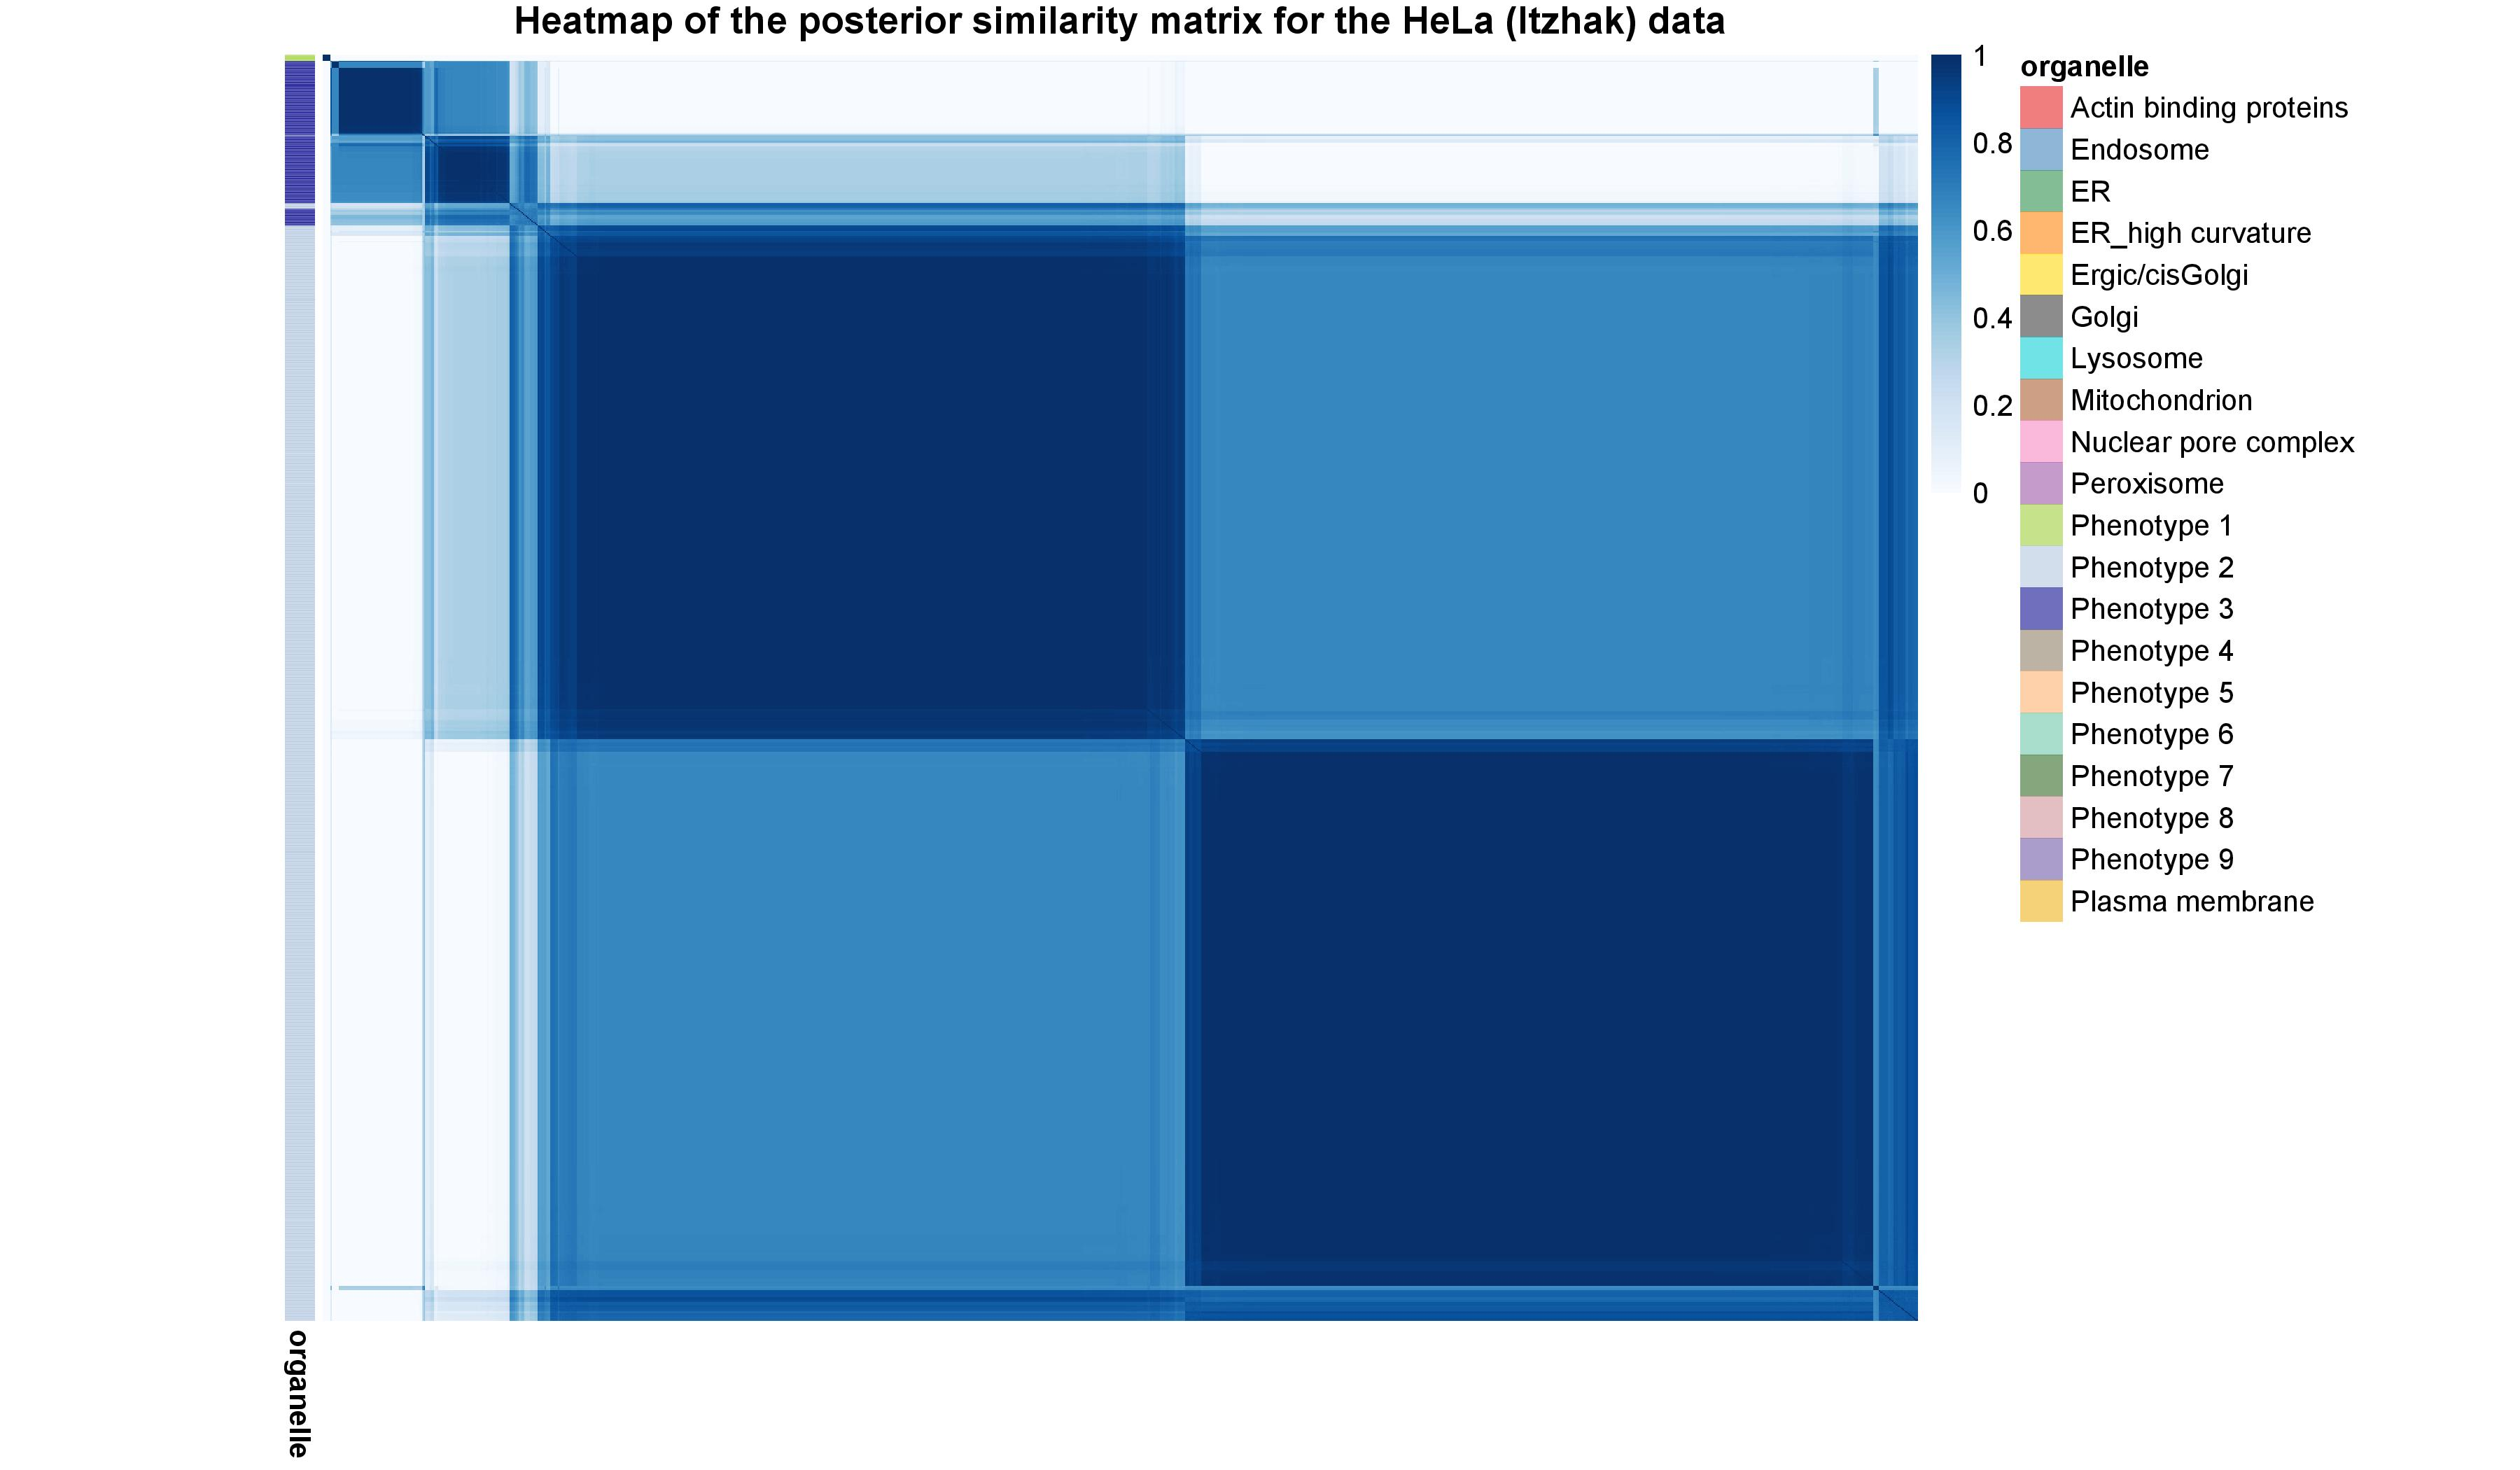
\includegraphics[height=2in]{itzhak2016heatmap.jpg}
		\caption{}
	\end{subfigure}
	~
	\begin{subfigure}[t]{0.5\textwidth}
		\centering
		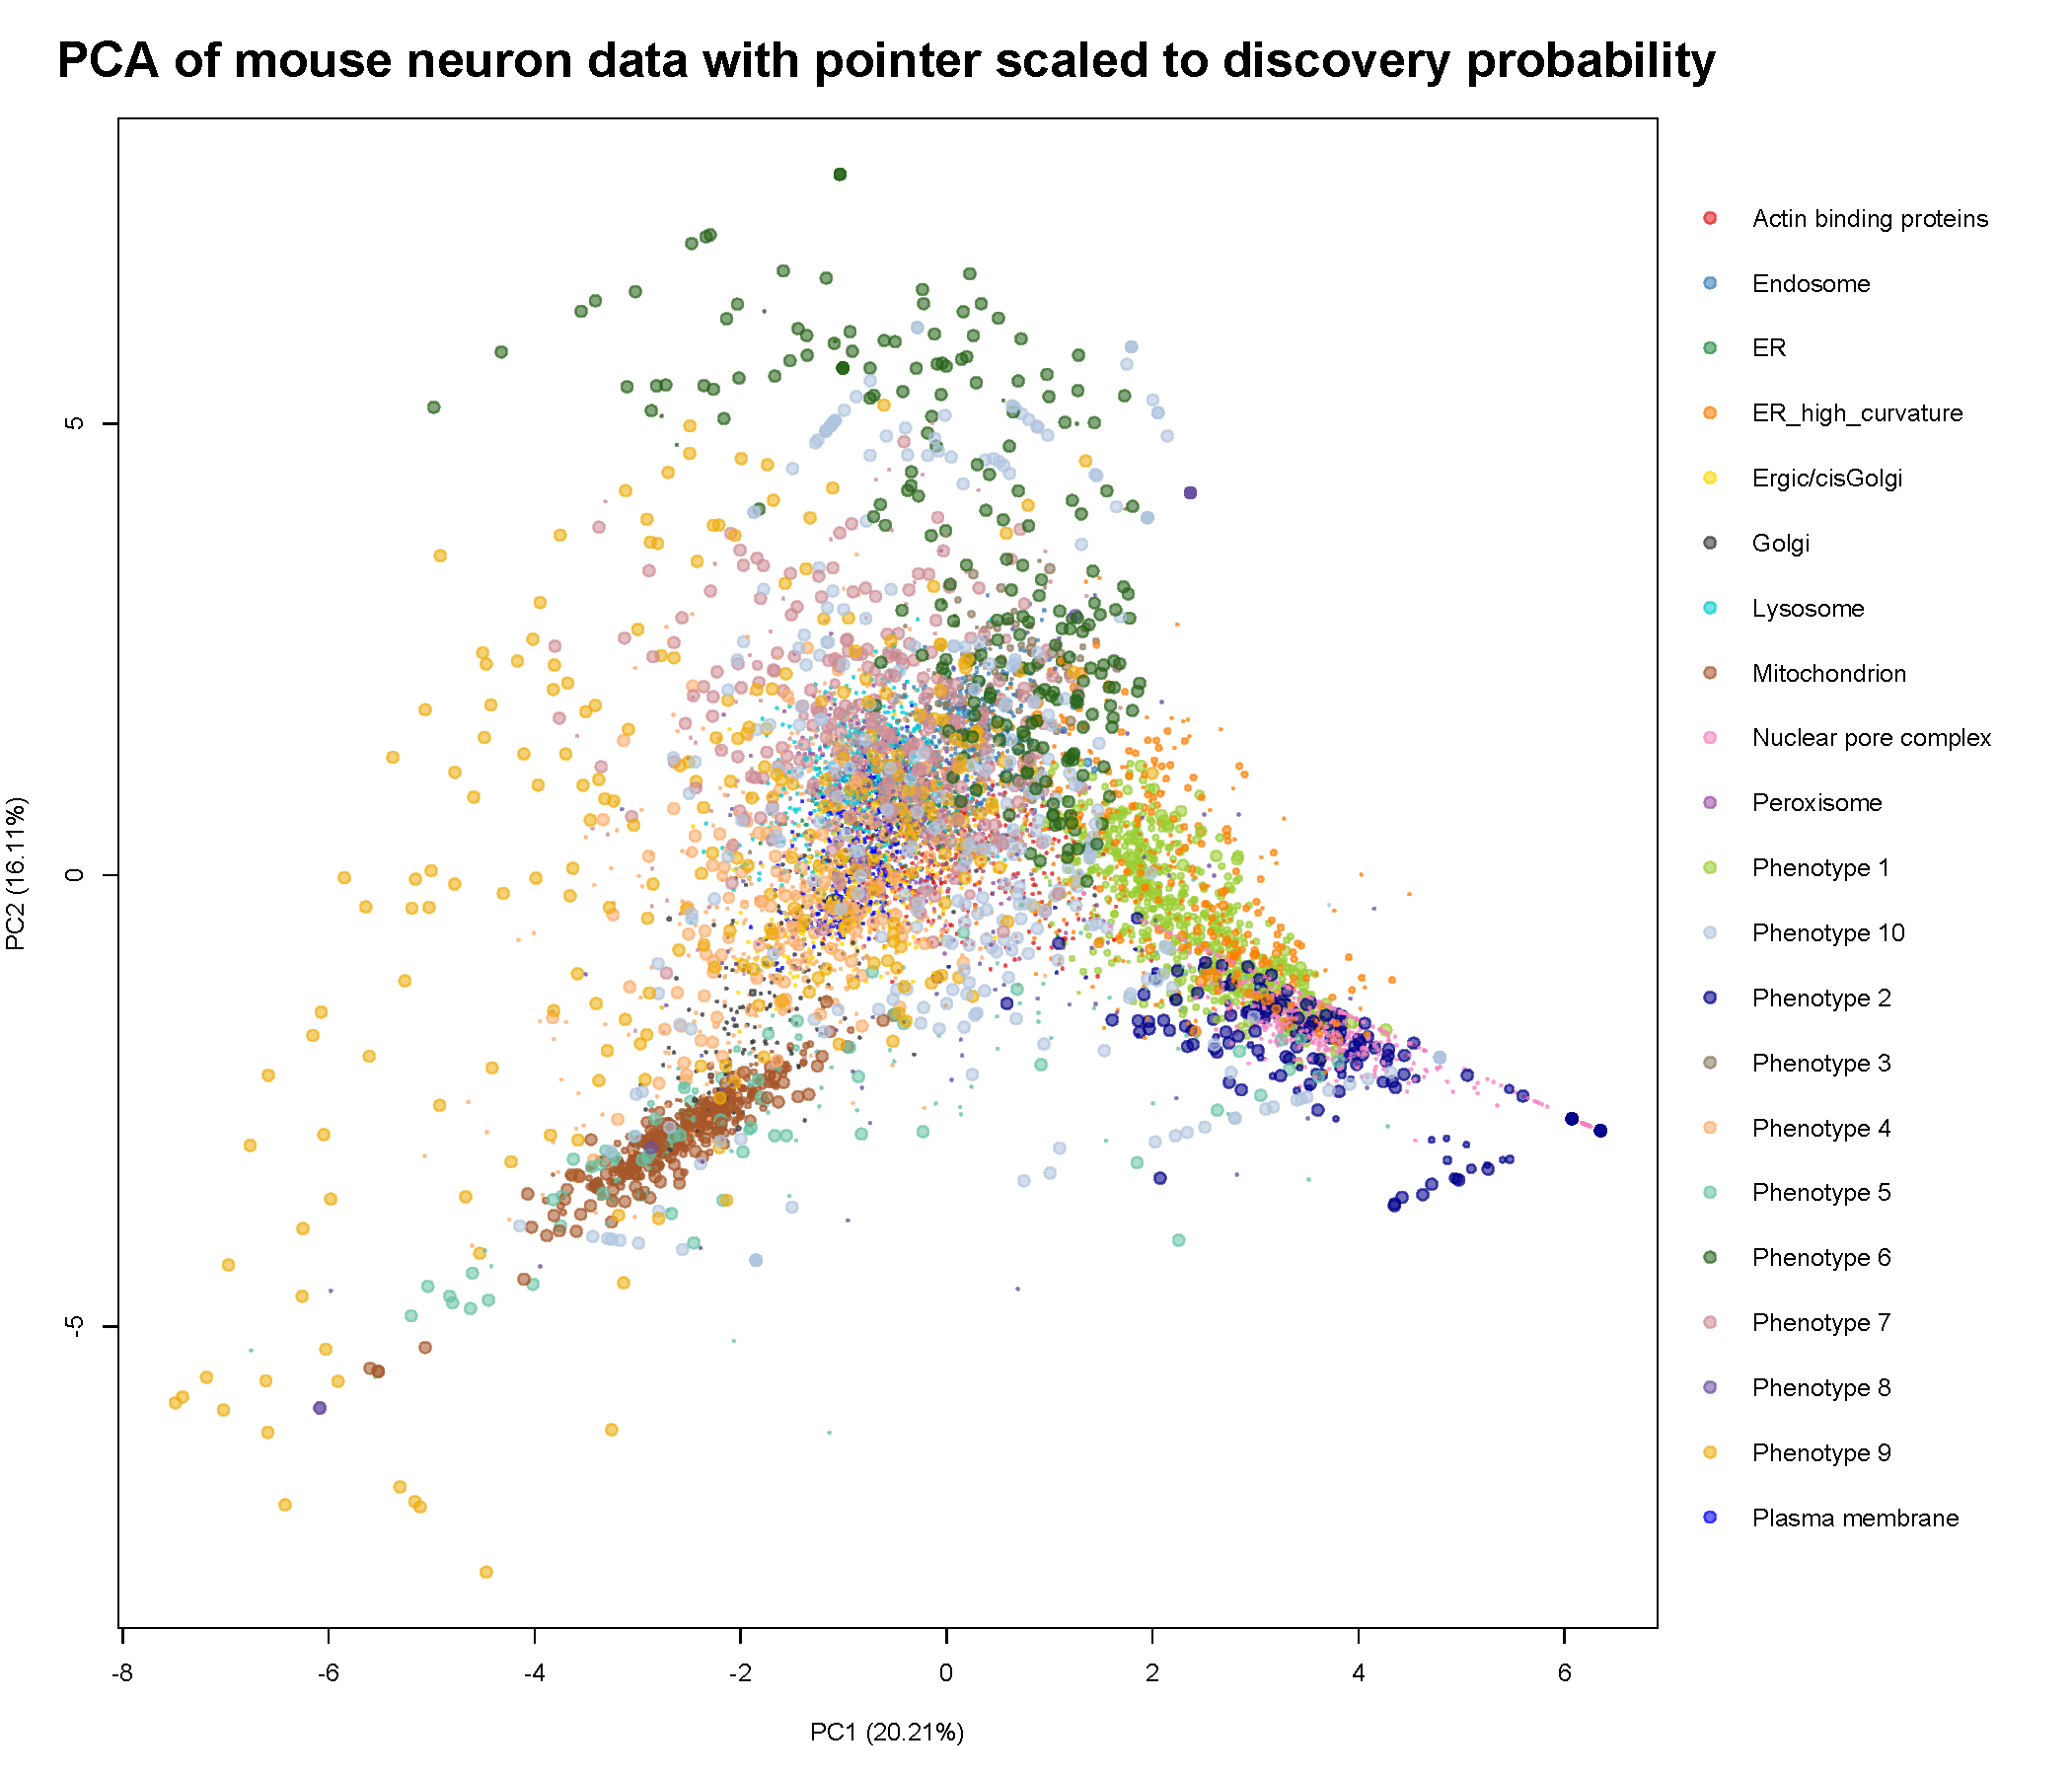
\includegraphics[height=2in]{pcaItzhak2017.pdf}
		\caption{}
	\end{subfigure}
	\begin{subfigure}[t]{0.5\textwidth}
		\centering
		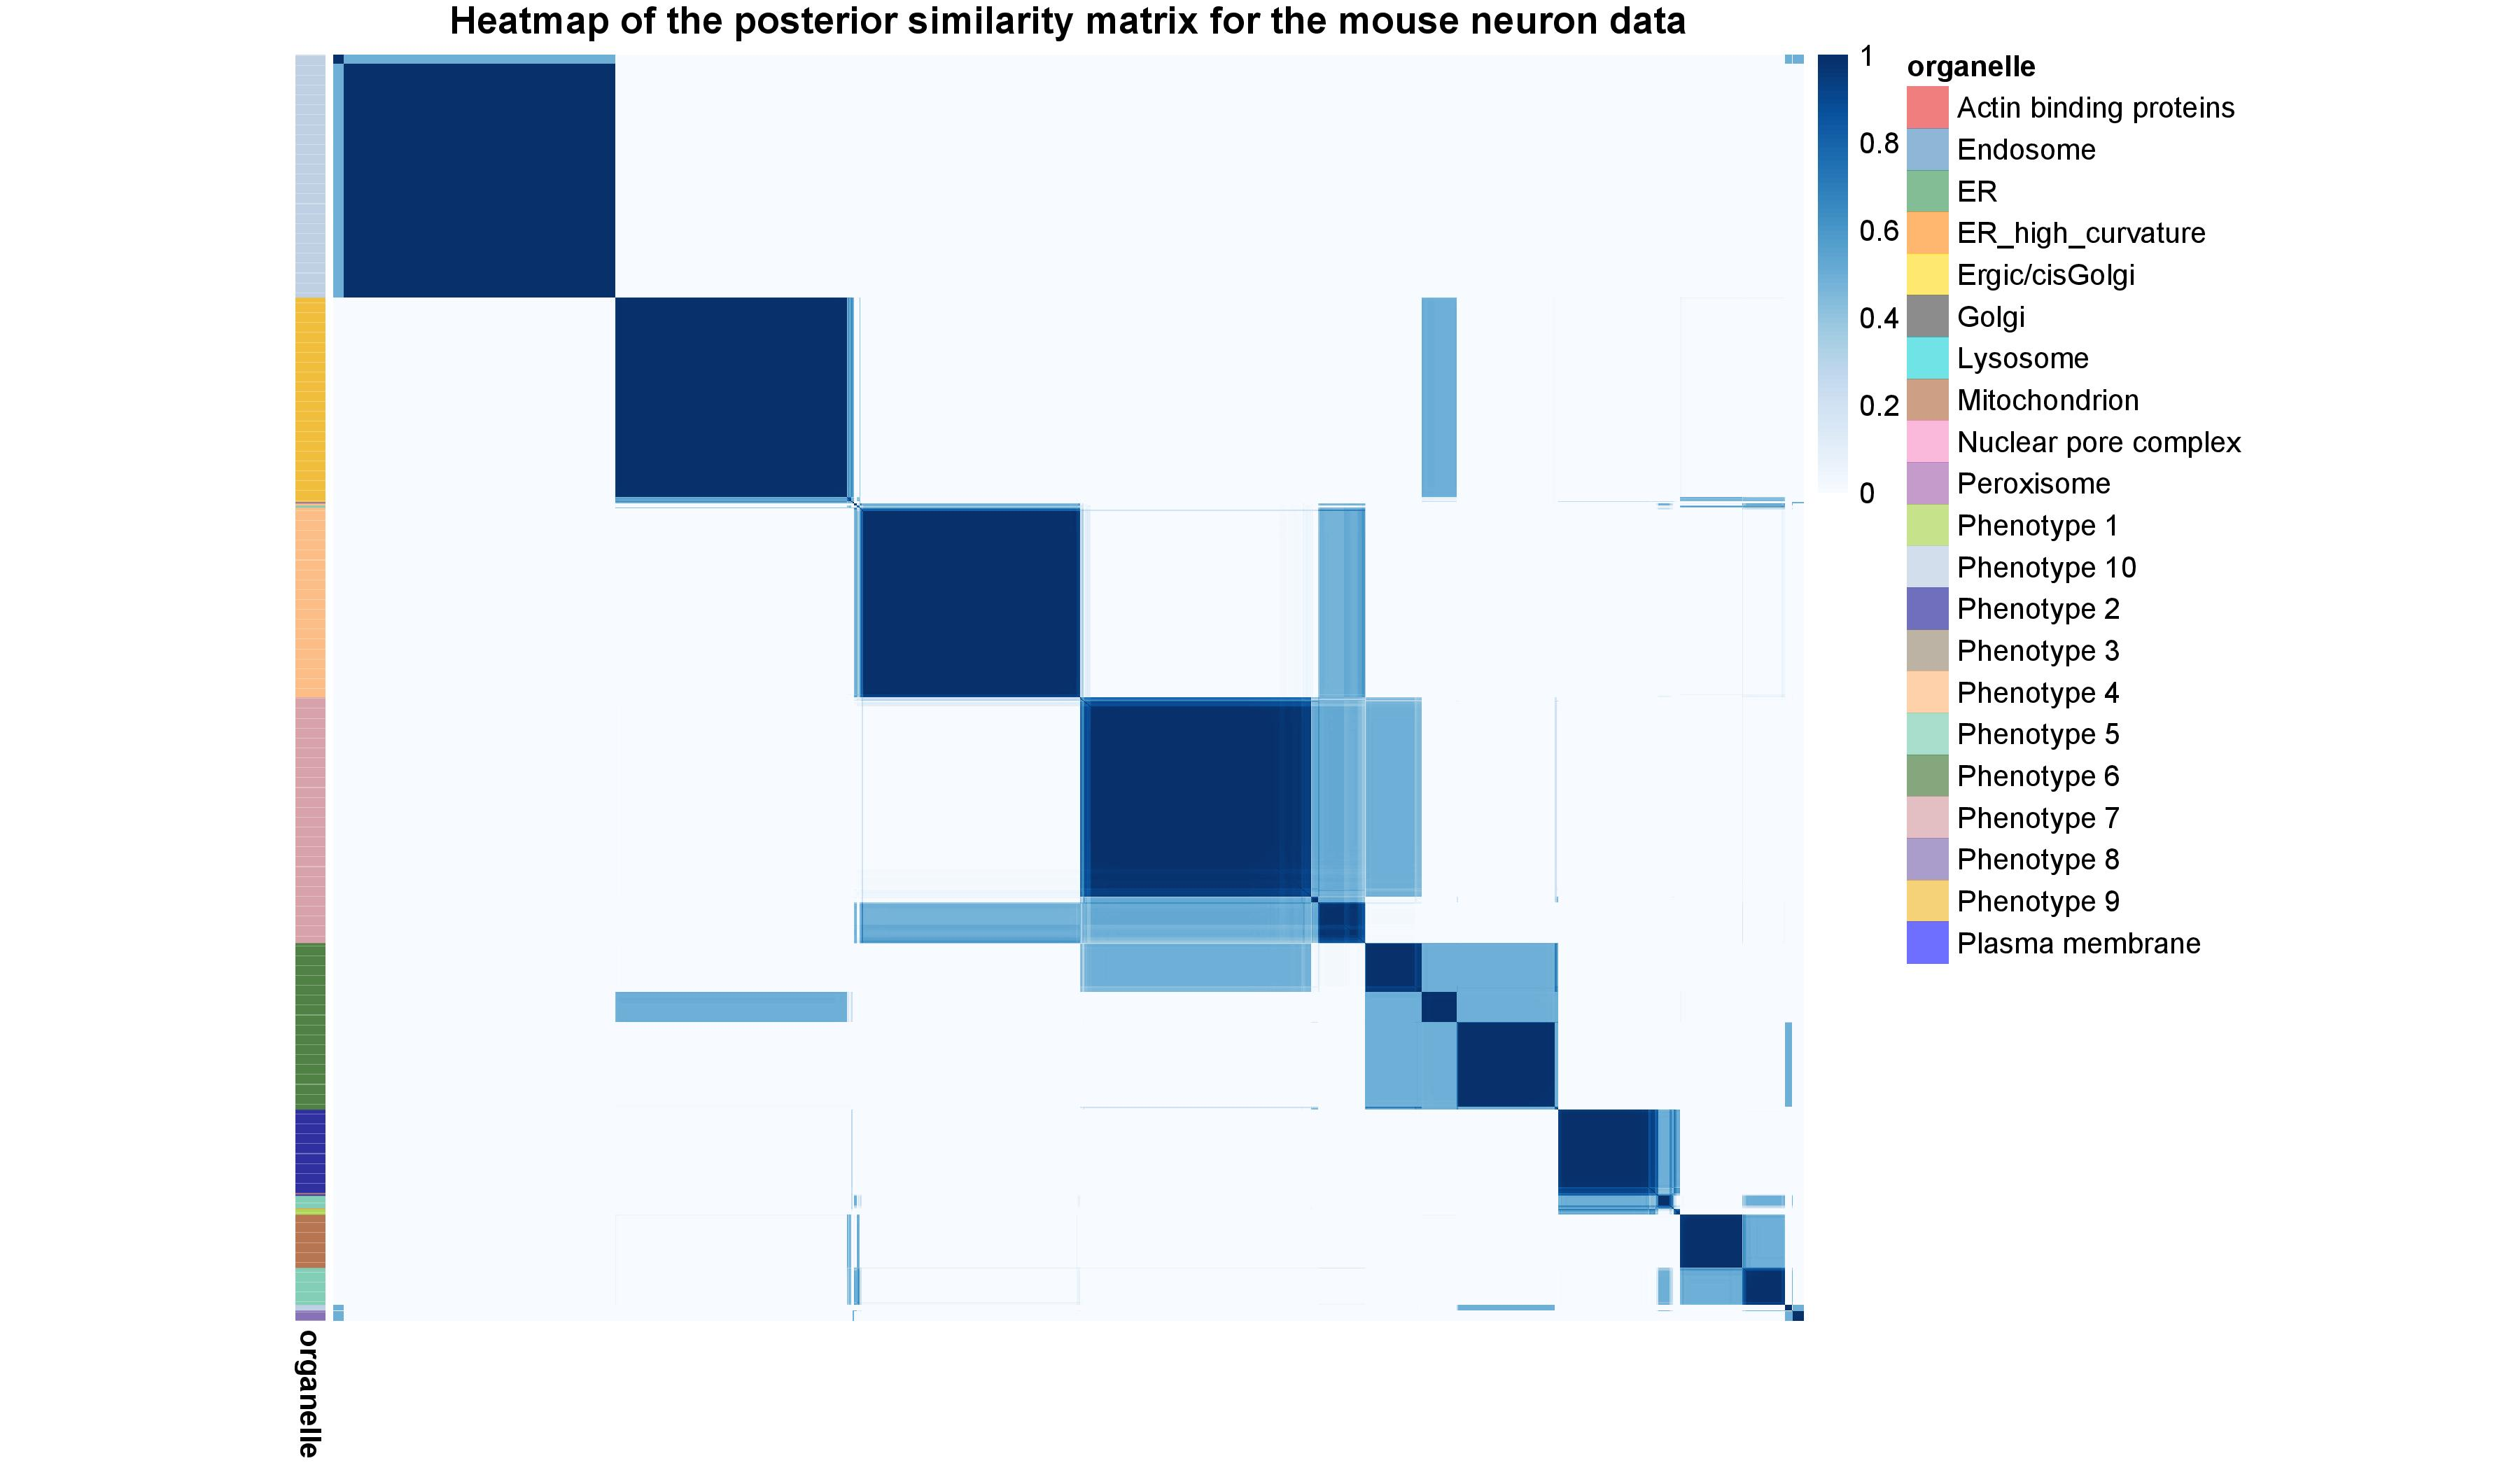
\includegraphics[height=2in]{heatmapItzhak2017.jpg}
		\caption{}
	\end{subfigure}
	~
	\begin{subfigure}[t]{0.5\textwidth}
		\centering
		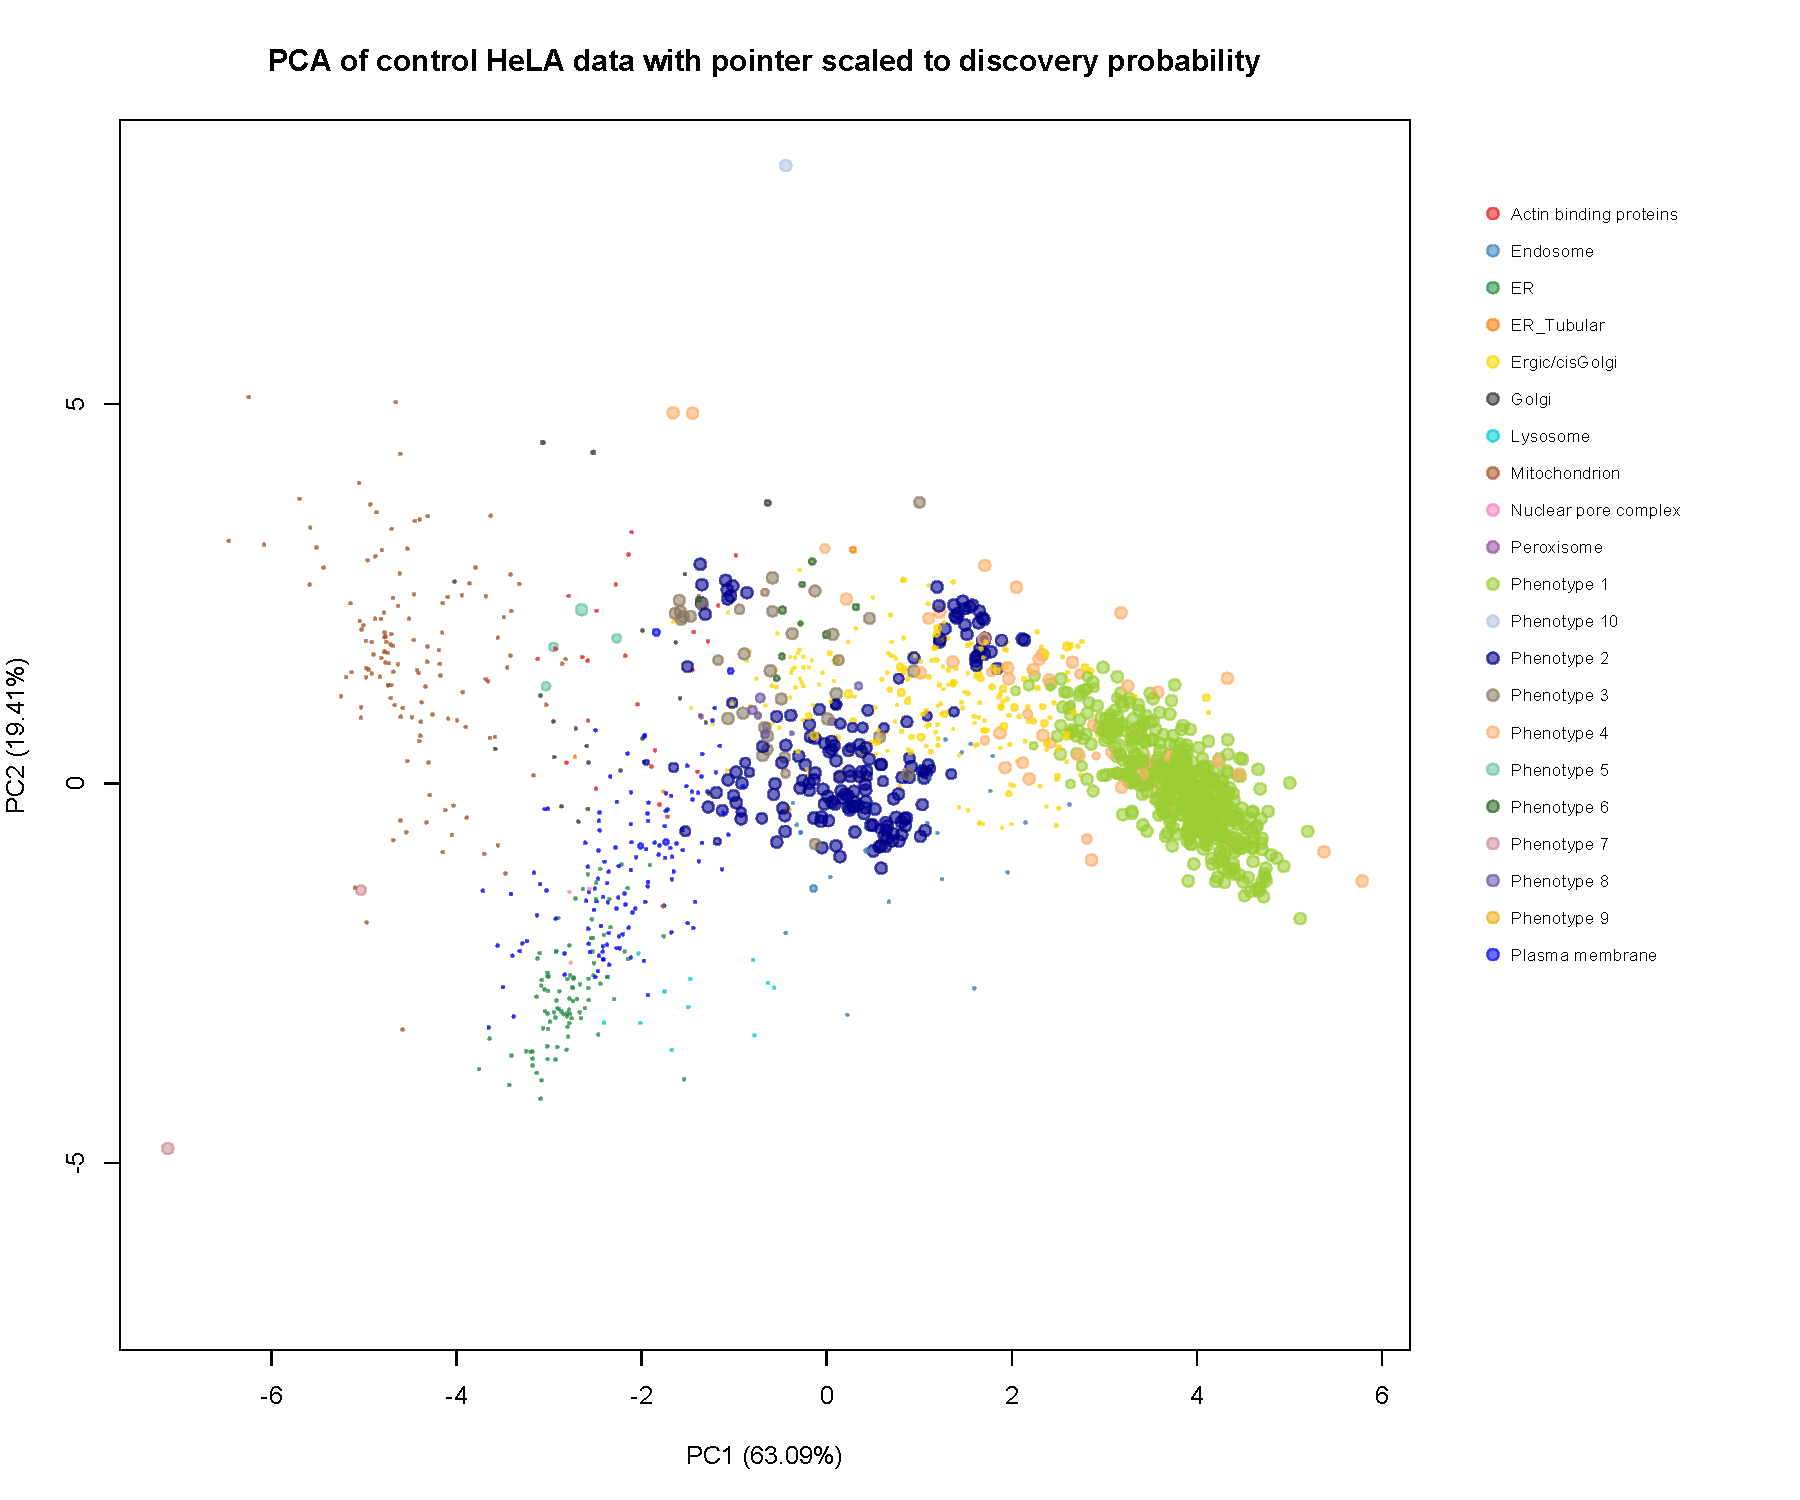
\includegraphics[height=2in]{pcaHirst.pdf}
		\caption{}
	\end{subfigure}
	\begin{subfigure}[t]{0.5\textwidth}
		\centering
		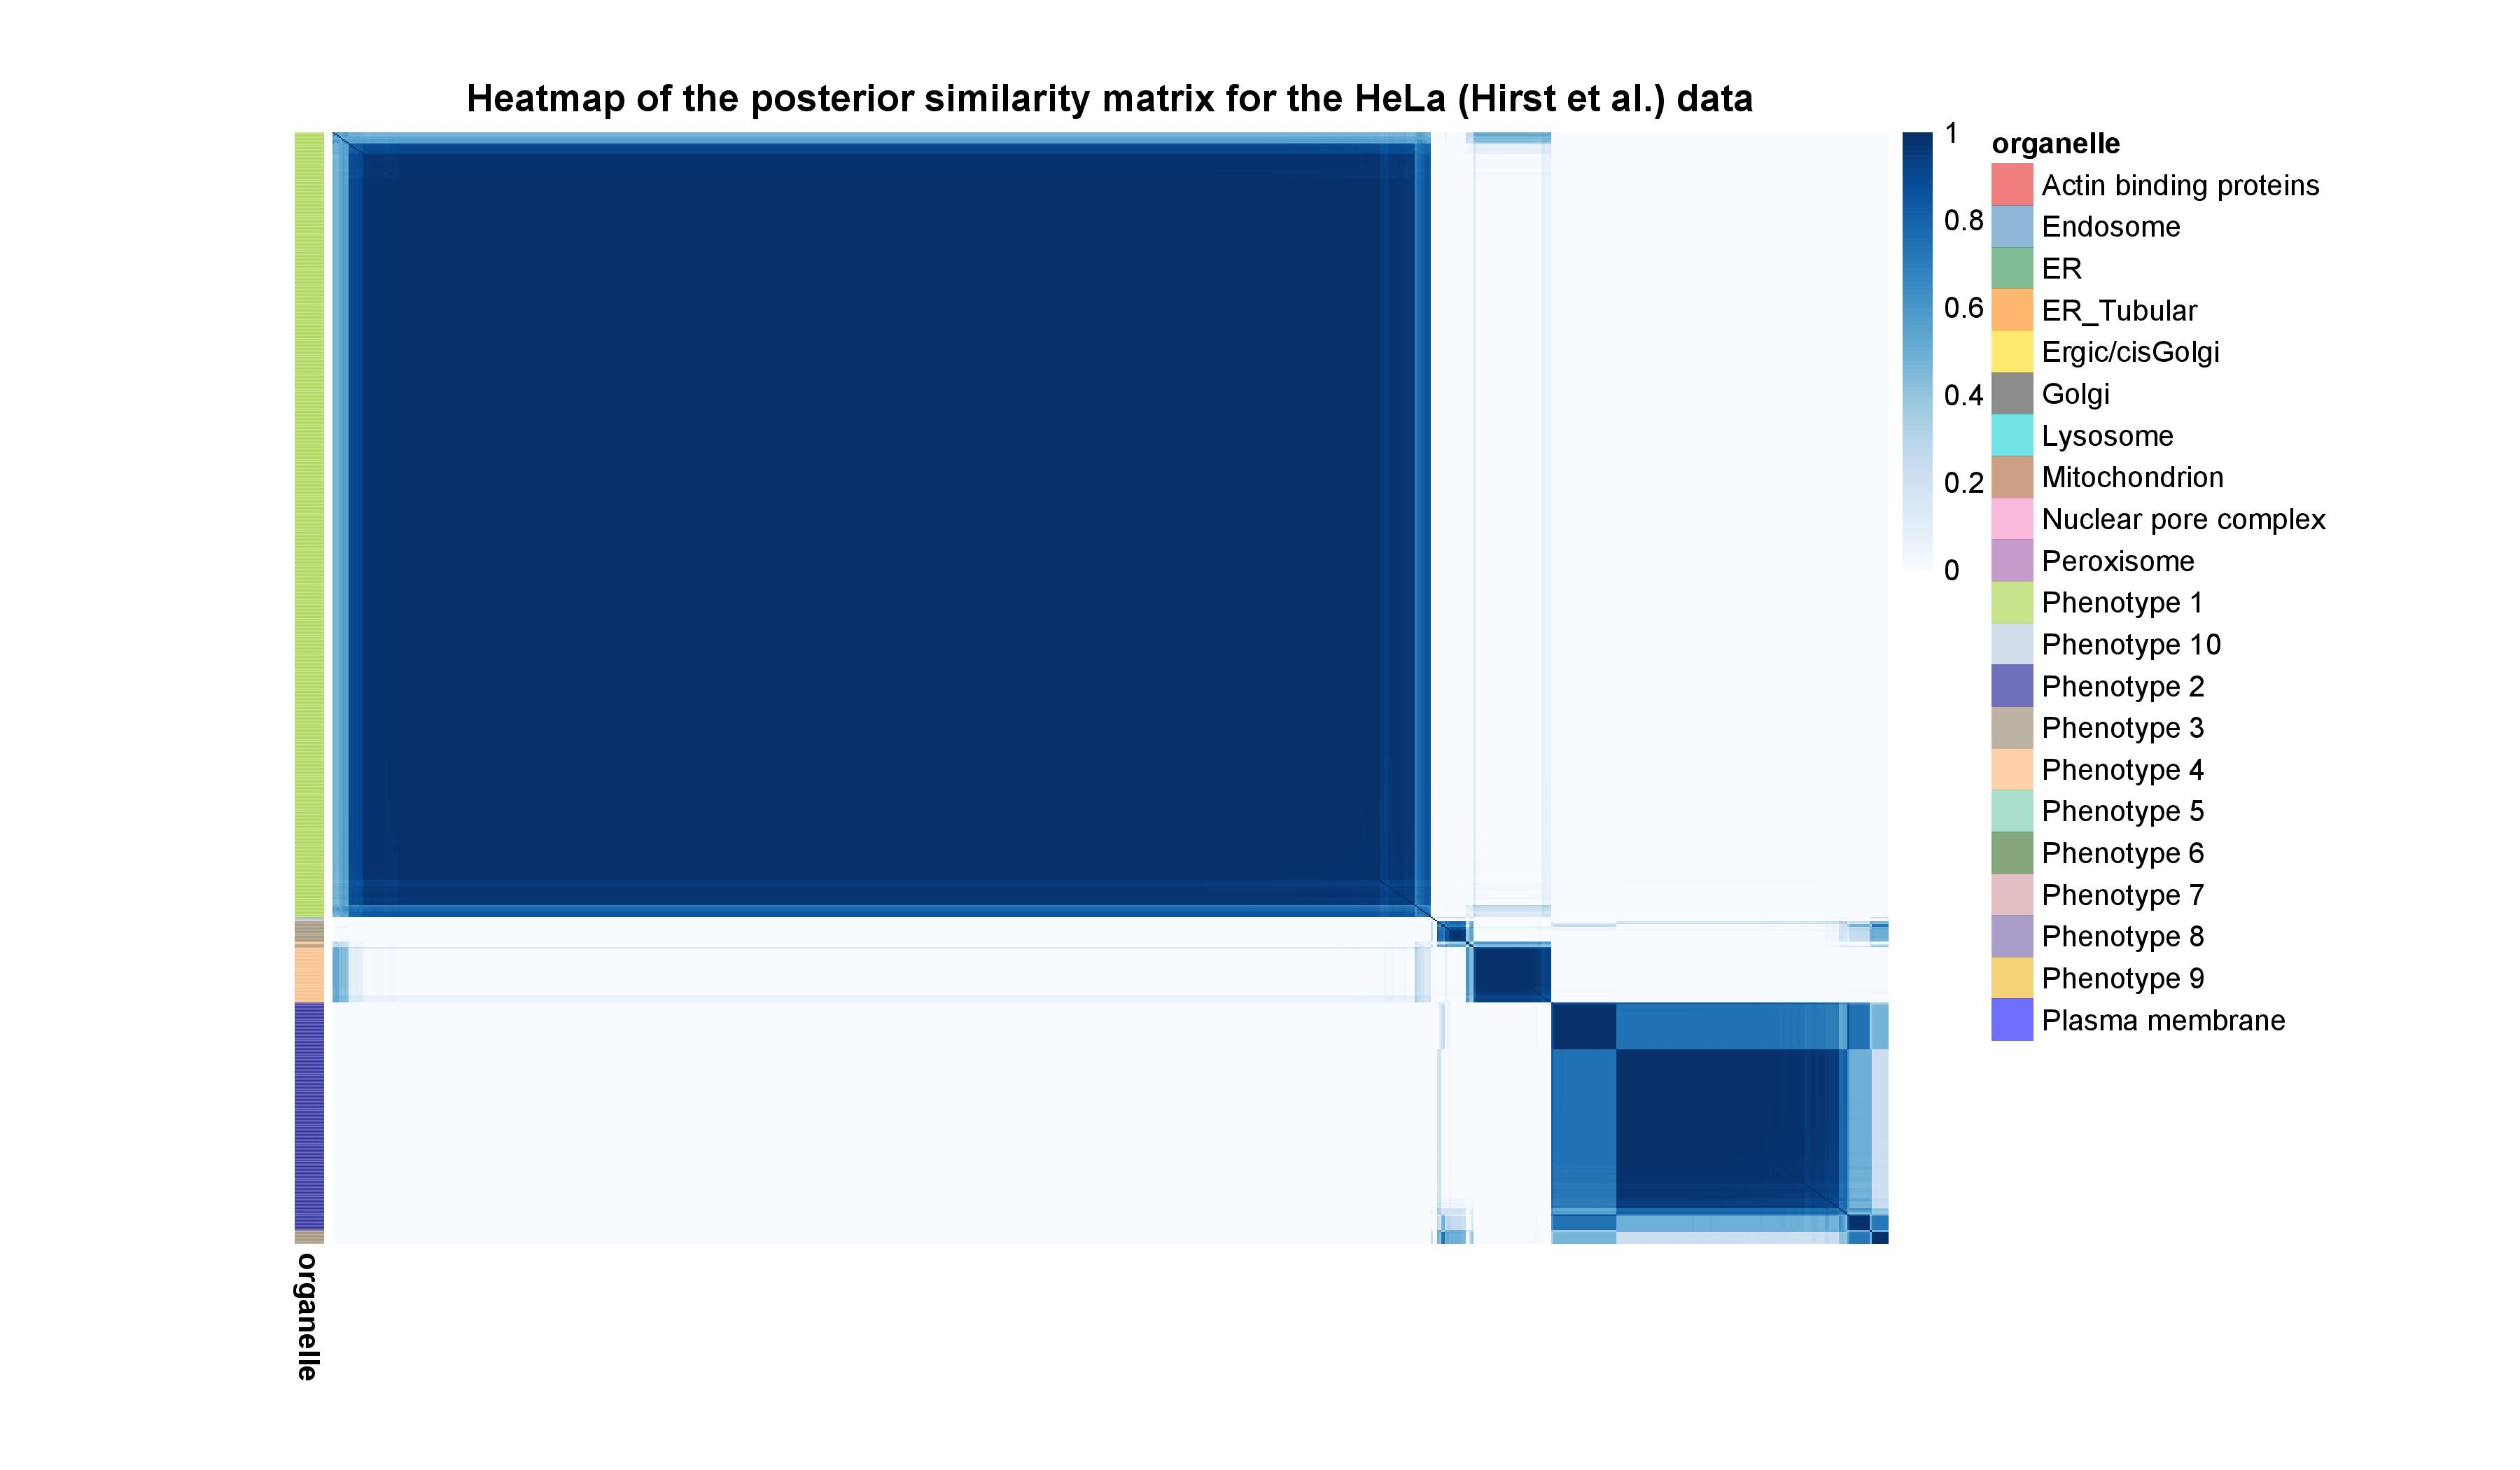
\includegraphics[height=2in]{heatmapHirst.jpg}
		\caption{}
	\end{subfigure}
	\caption{(a),(c),(e) PCA plots of the HeLa Itzhak data, mouse primary neuron data and HeLa Hirst data. The pointers are coloured according to the assigned organelle or phenotype and scaled according to their discovery probability. (b),(d),(f) Heatmaps of the HeLa Itzhak data, mouse neuron data and HeLa Hirst data. Only the proteins whos discovery probability is greater than $0.99$ and outlier probability less than $0.95$ ($10^{-2}$ for the mouse primary neuron dataset to reduce the number of visualised proteins) are shown. The heatmaps demonstrate the uncertainty in the clustering structure present in the data.}
	\label{figure:DOM}
\end{figure}
\clearpage
\section{Comparison between Novelty TAGM and \textit{phenoDisco}}
In this section, we compare an already available novelty detection algorithm, \textit{phenoDisco}, with Novelty TAGM. Despite both methods performing novelty detection, the algorithms
are quite distinct. The first major difference is that Novelty TAGM is a Bayesian 
method and as a result performs uncertainty quantification. Novelty TAGM quantifies the uncertainty in both the number of newly identified phenotypes and whether individual proteins should belong to a new phenotypes. On the other hand, \textit{phenoDisco} must use the heuristic \textit{Bayesian Information Criterion} BIC to decide the number of phenotypes and does not provide an estimate of individual protein-to-phenotype allocation uncertainty. Another difference is the input to both methods; Novelty TAGM uses the data directly, whereas \textit{phenoDisco} takes the first two principal components as input. \textit{PhenoDisco} also requires an additional parameter - the minimum group size. This parameter can be challenging to specify, since there is a trade-off between identifying functionally relevant phenotypes of different sizes and picking up small spurious protein clusters. Furthermore, \textit{phenoDisco} struggles to scale to many of the datasets presented in this manuscript, because it requires iteratively refitting models and building of an outlier test statistic. 

To demonstrate the difference between the two approaches, we apply \textit{phenoDisco} and Novelty TAGM to a spatial proteomics dataset on HEK-293 cells \citep{Breckels:2013}. The PCA plots in figure \ref{figure:phenodisco} reveal broad similarities in the location of the discovered phenotypes. Clearly, Novelty TAGM provides more information by scaling the pointer size to the discovery probability. We note that both methods reveal 8 phenotypes in the data, where for Novelty TAGM a phenotype needs at least one protein with discovery probability greater than $0.95$. Figure \ref{figure:phenodisco} (panels d and e) reveals the distribution of proteins across these phenotypes. We conclude that both approaches are able to discover small and large phenotypes without difficulty, with both methods identifying phenotypes with a few proteins, but also phenotypes with greater than 100 proteins. Figure \ref{figure:phenodisco} (panel f) shows that both methods find the same number of phenotypes; however, not all of these phenotypes are functionally enriched. For \textit{phenoDisco} $4$ of the phenotypes had at least 1 significant Gene Ontology term, whereas this was true for $5$ of the Novelty TAGM phenotypes. Figure \ref{figure:phenodisco} (panel g) characterises the protein overlap between the two approaches. We see that both methods are in broad agreement, with most of the disagreement attributed to cases where one method assigns a protein as unknown whilst the other allocates to it a phenotype or organelle. For example, Novelty TAGM associates \textit{phenoDisco} phenotype 3, which is a Lysosome-enriched phenotype, with the PM. On the other hand, Novelty TAGM phenotypes 2 and 3, enriched for chromatin and ribosome respectively, are associated with the mitochondria by \textit{phenoDisco}.

\begin{figure}
	\begin{subfigure}[t]{0.33\textwidth}
		\centering
		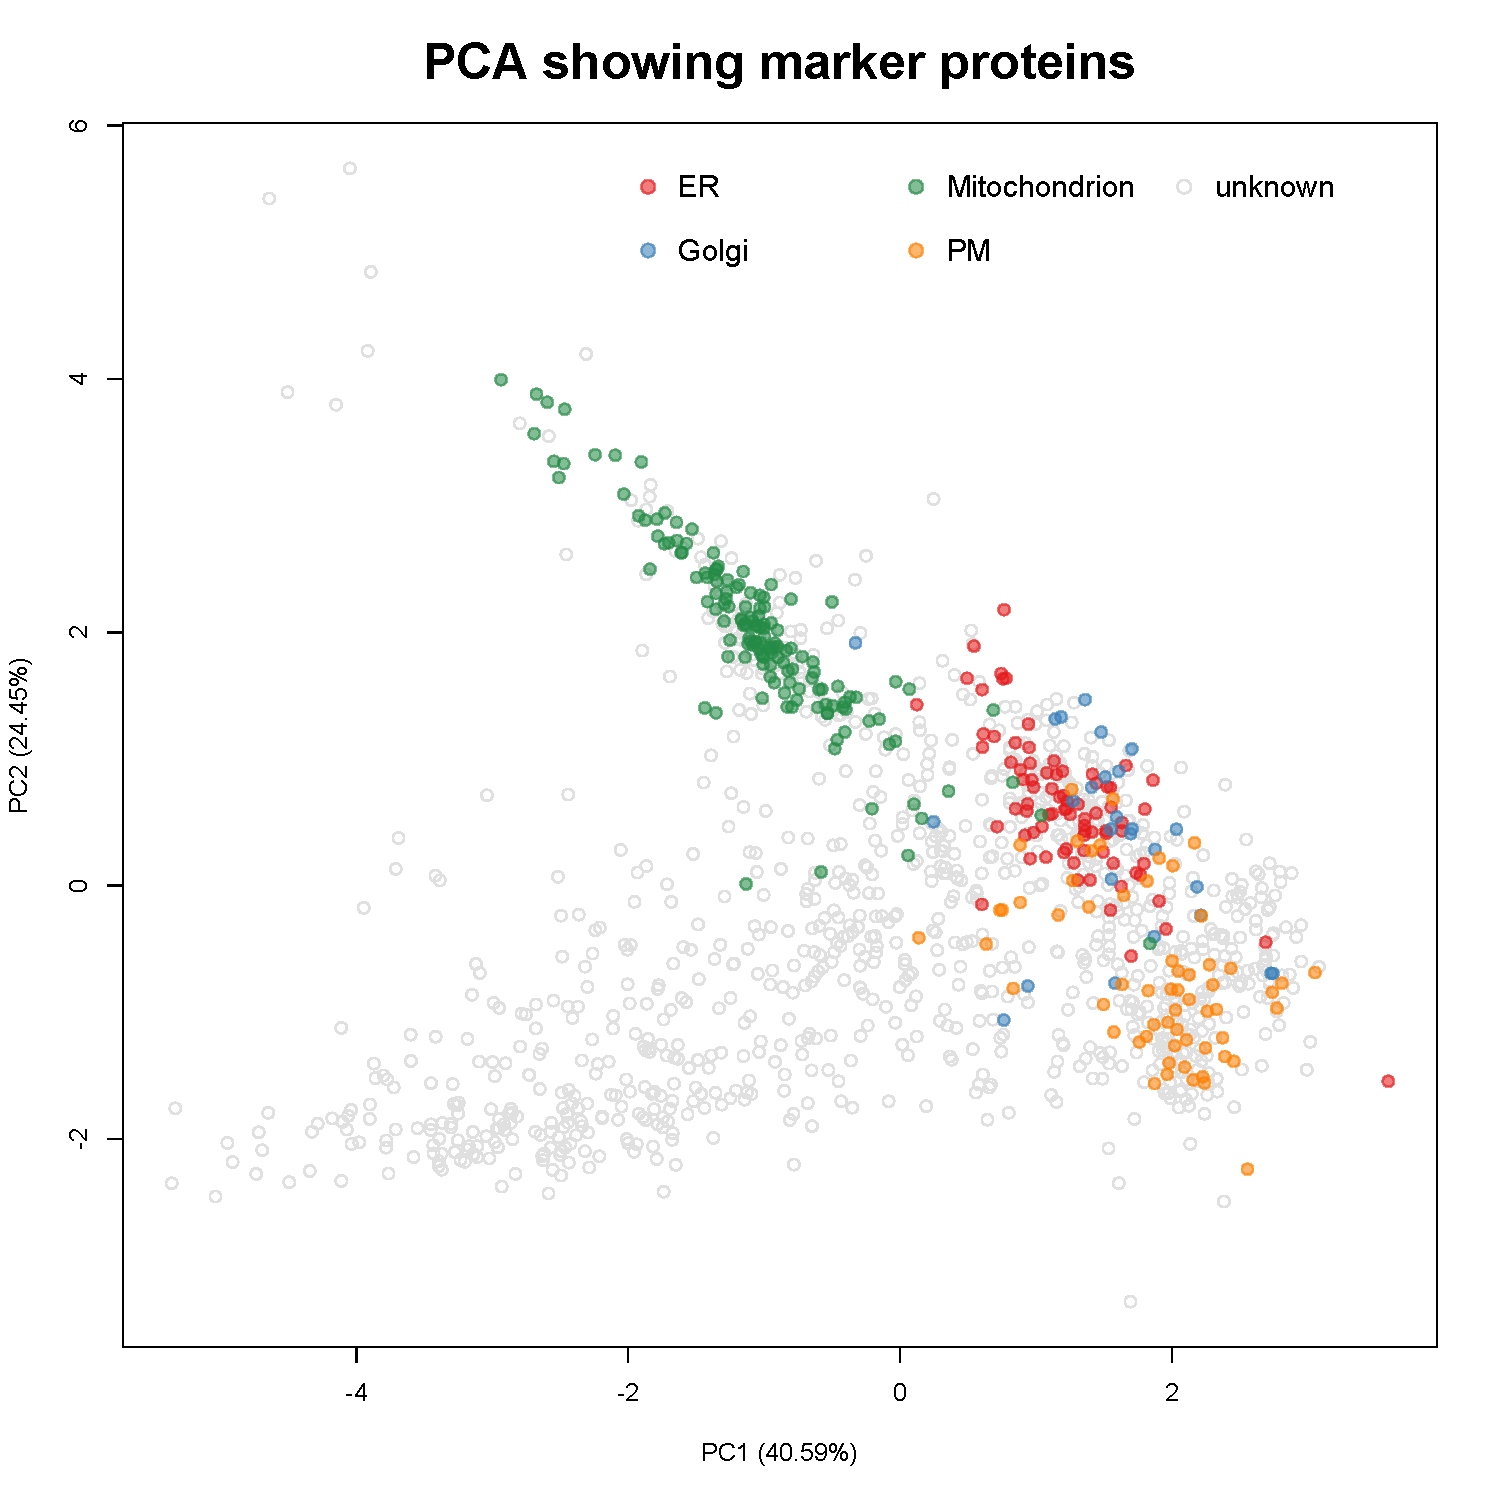
\includegraphics[height=2in]{pcaMarkershek}
		\caption{}
	\end{subfigure}%
	\begin{subfigure}[t]{0.33\textwidth}
		\centering
		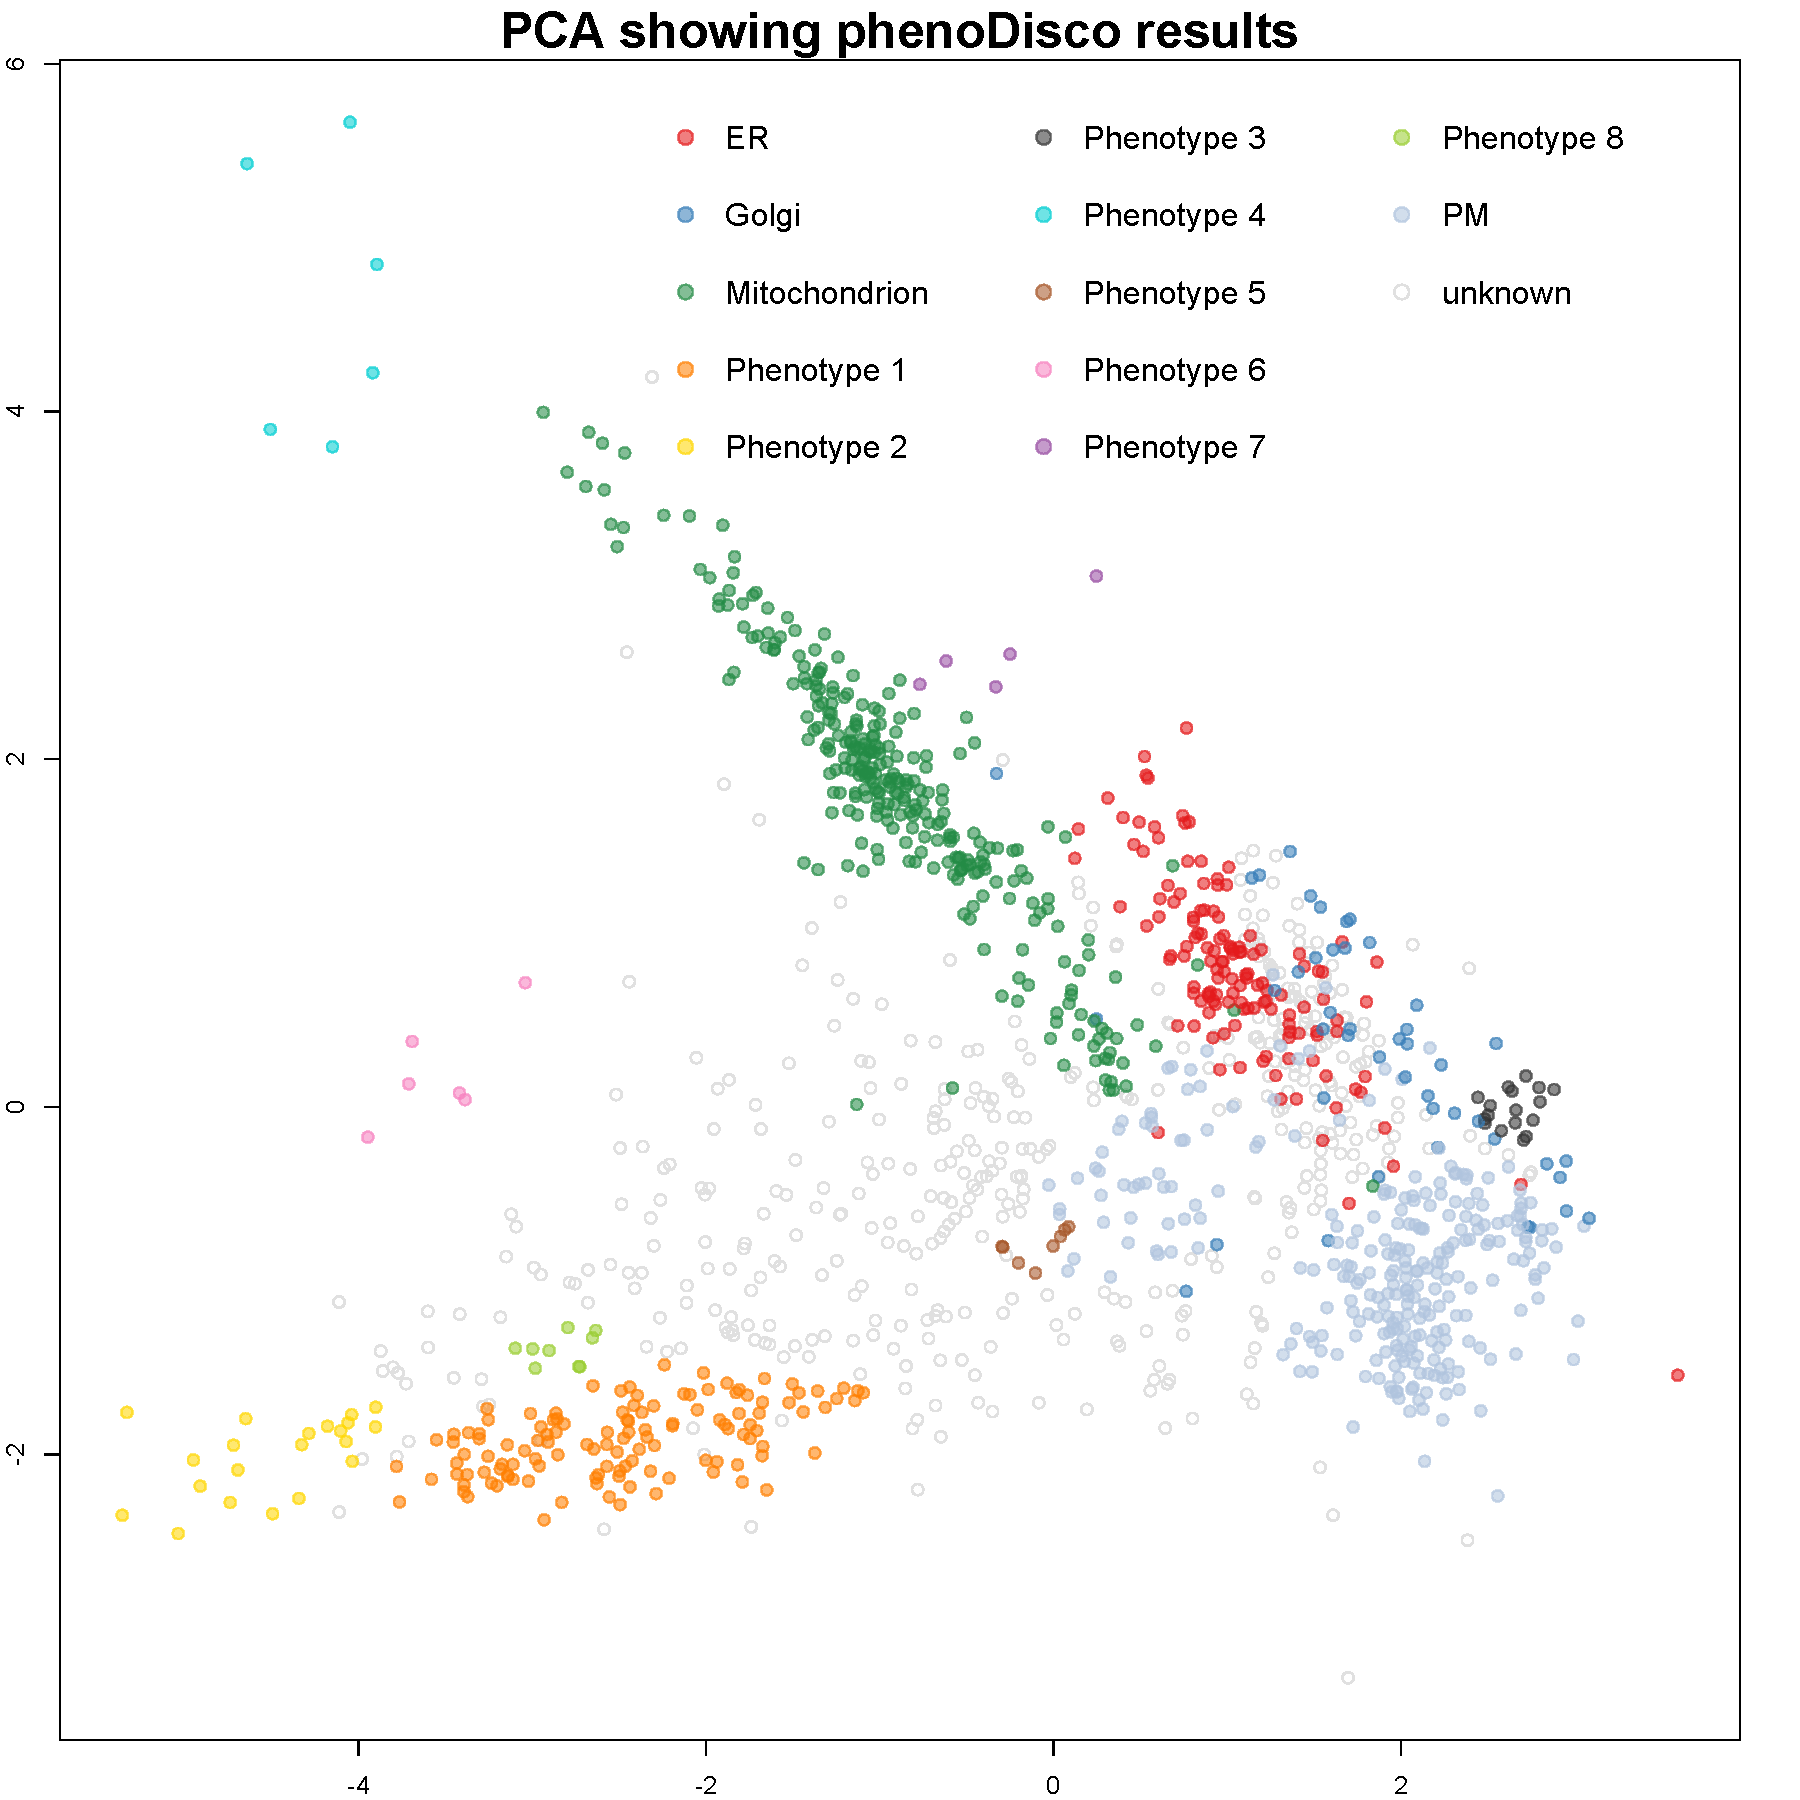
\includegraphics[height=2in]{pcaPDhek}
		\caption{}
	\end{subfigure}%
	\begin{subfigure}[t]{0.33\textwidth}
		\centering
		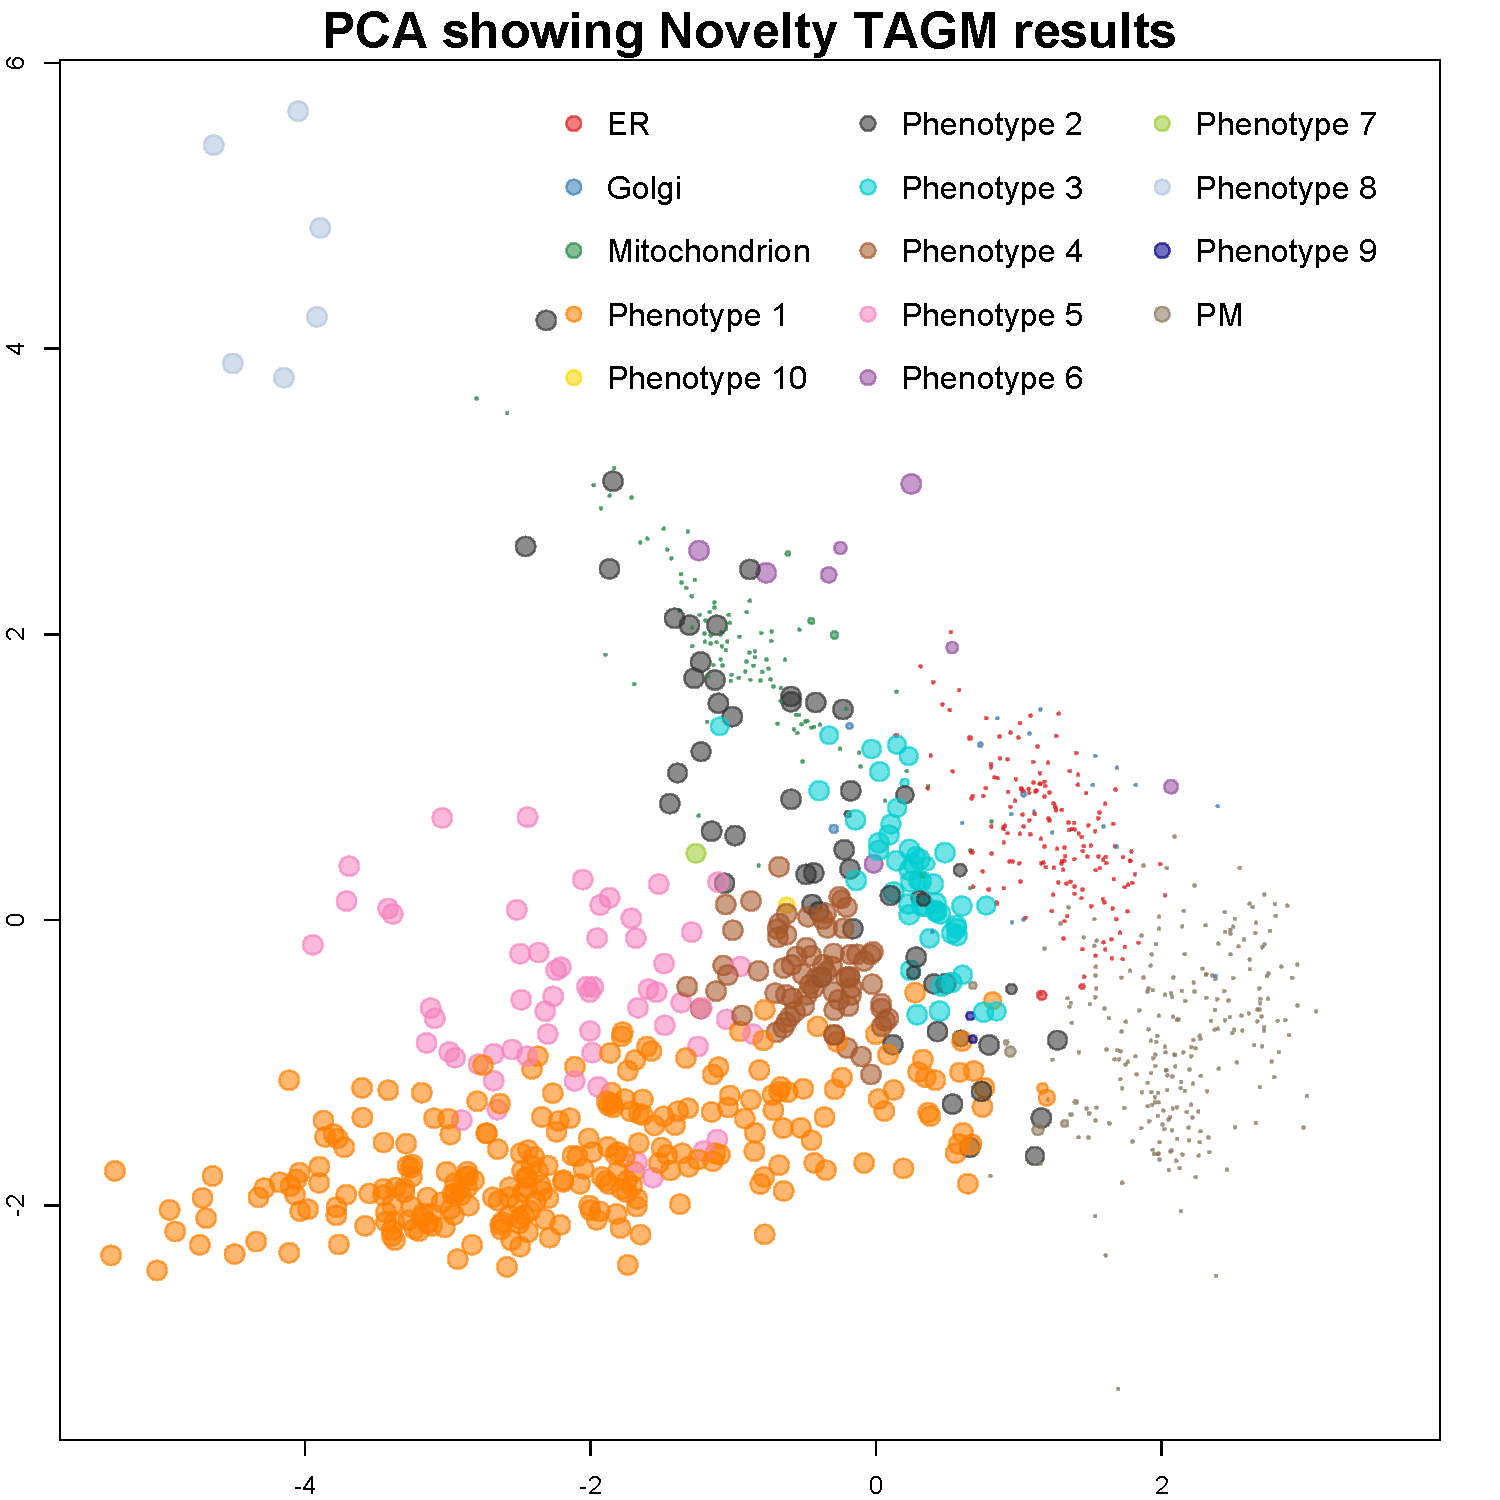
\includegraphics[height=2in]{pcaTAGMhek}
		\caption{}
	\end{subfigure}
~
	\begin{subfigure}[t]{0.5\textwidth}
		\centering
		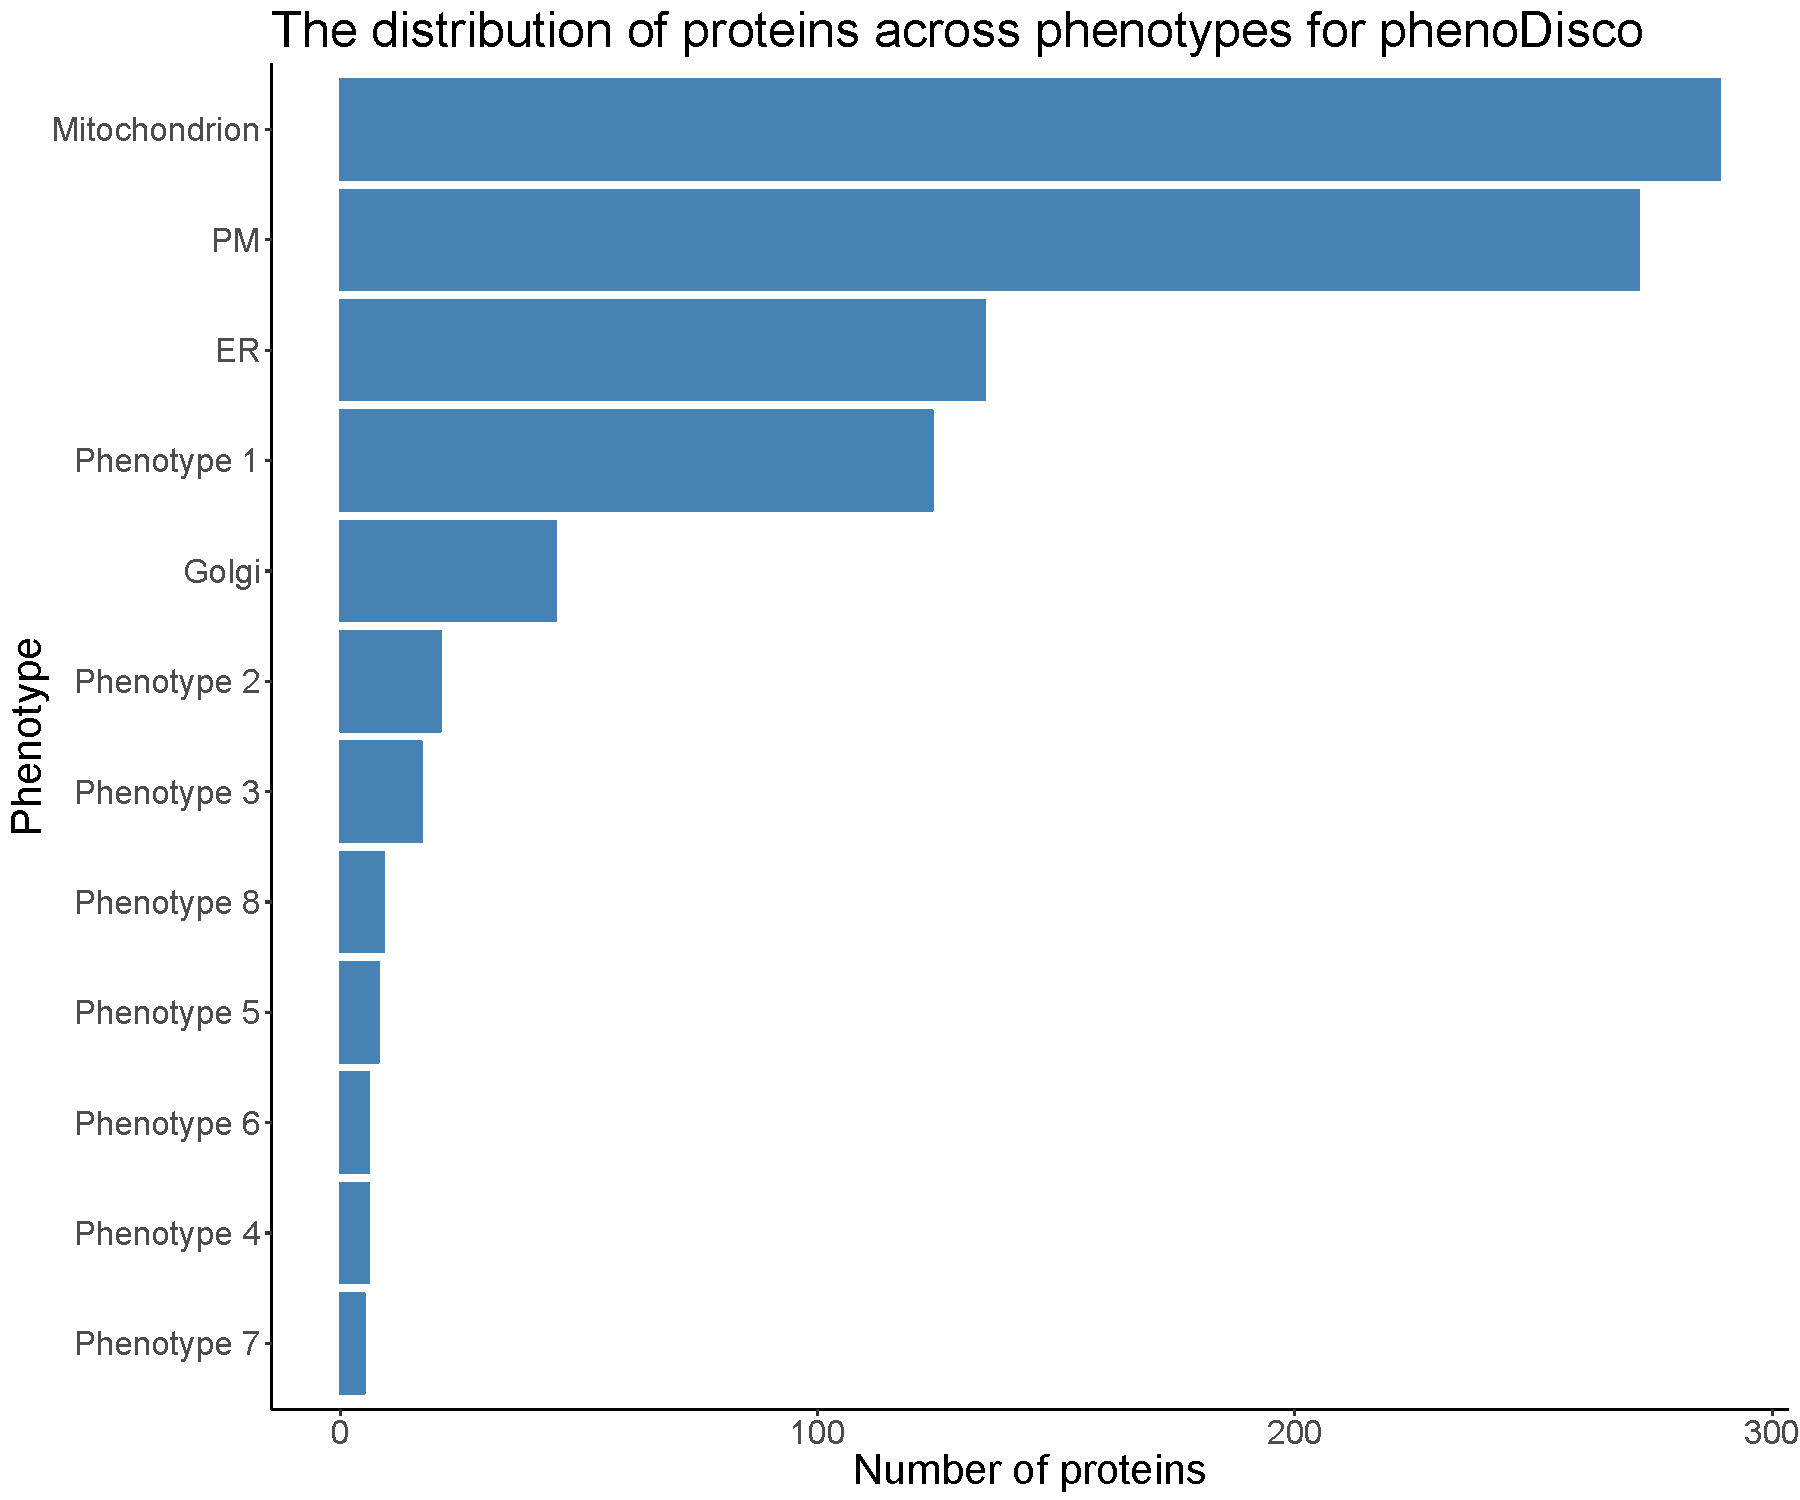
\includegraphics[height=2in]{phenodiscodist}
		\caption{}
	\end{subfigure}
	\begin{subfigure}[t]{0.5\textwidth}
		\centering
		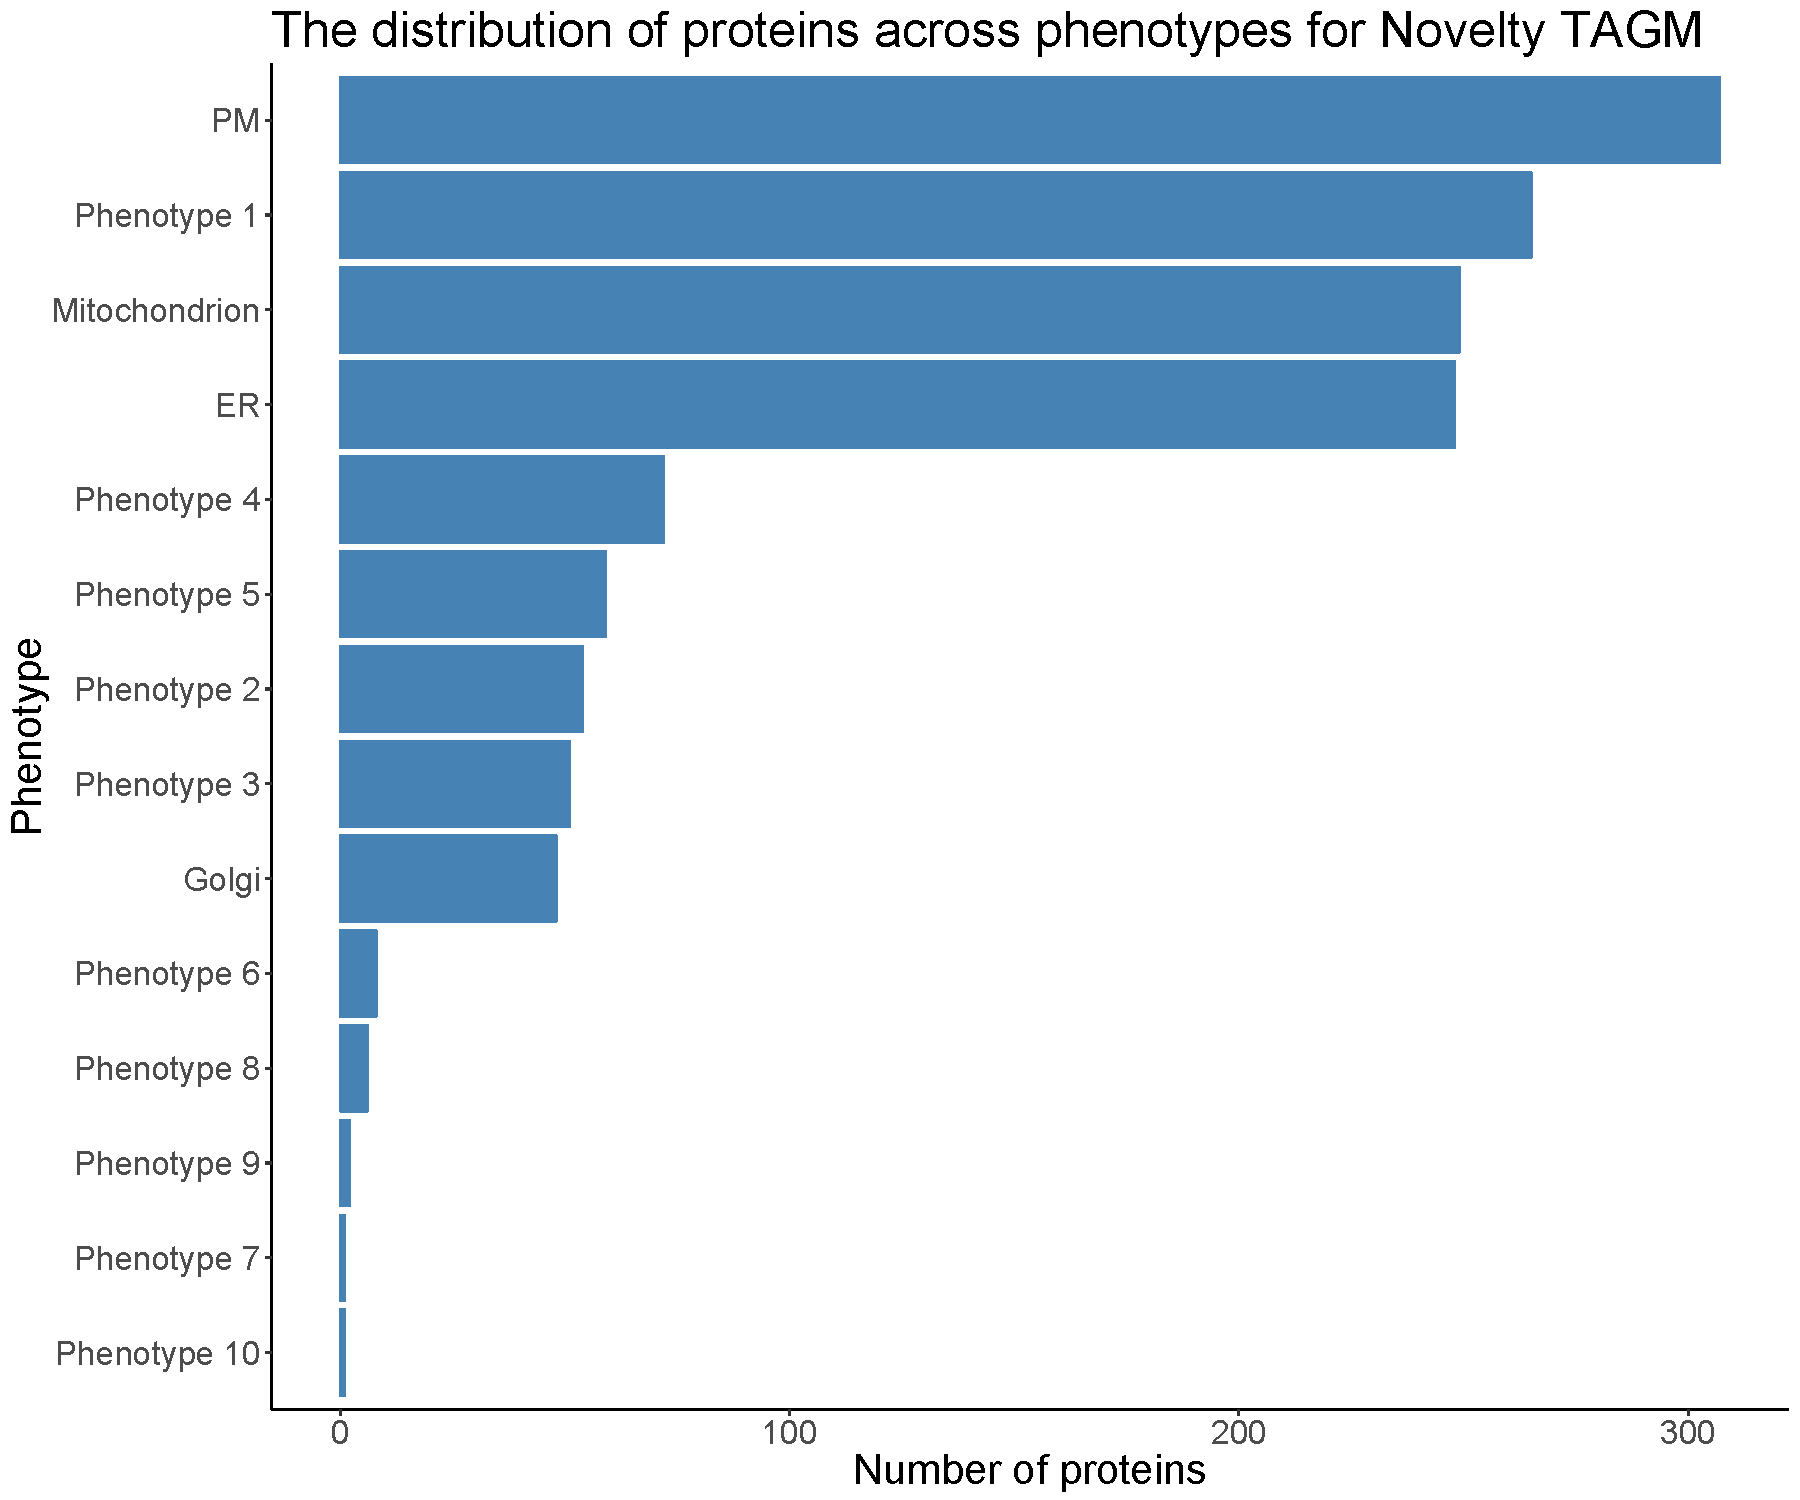
\includegraphics[height=2in]{noveltytagmdist}
		\caption{}
	\end{subfigure}	
~
\begin{subfigure}[t]{0.5\textwidth}
	\centering
	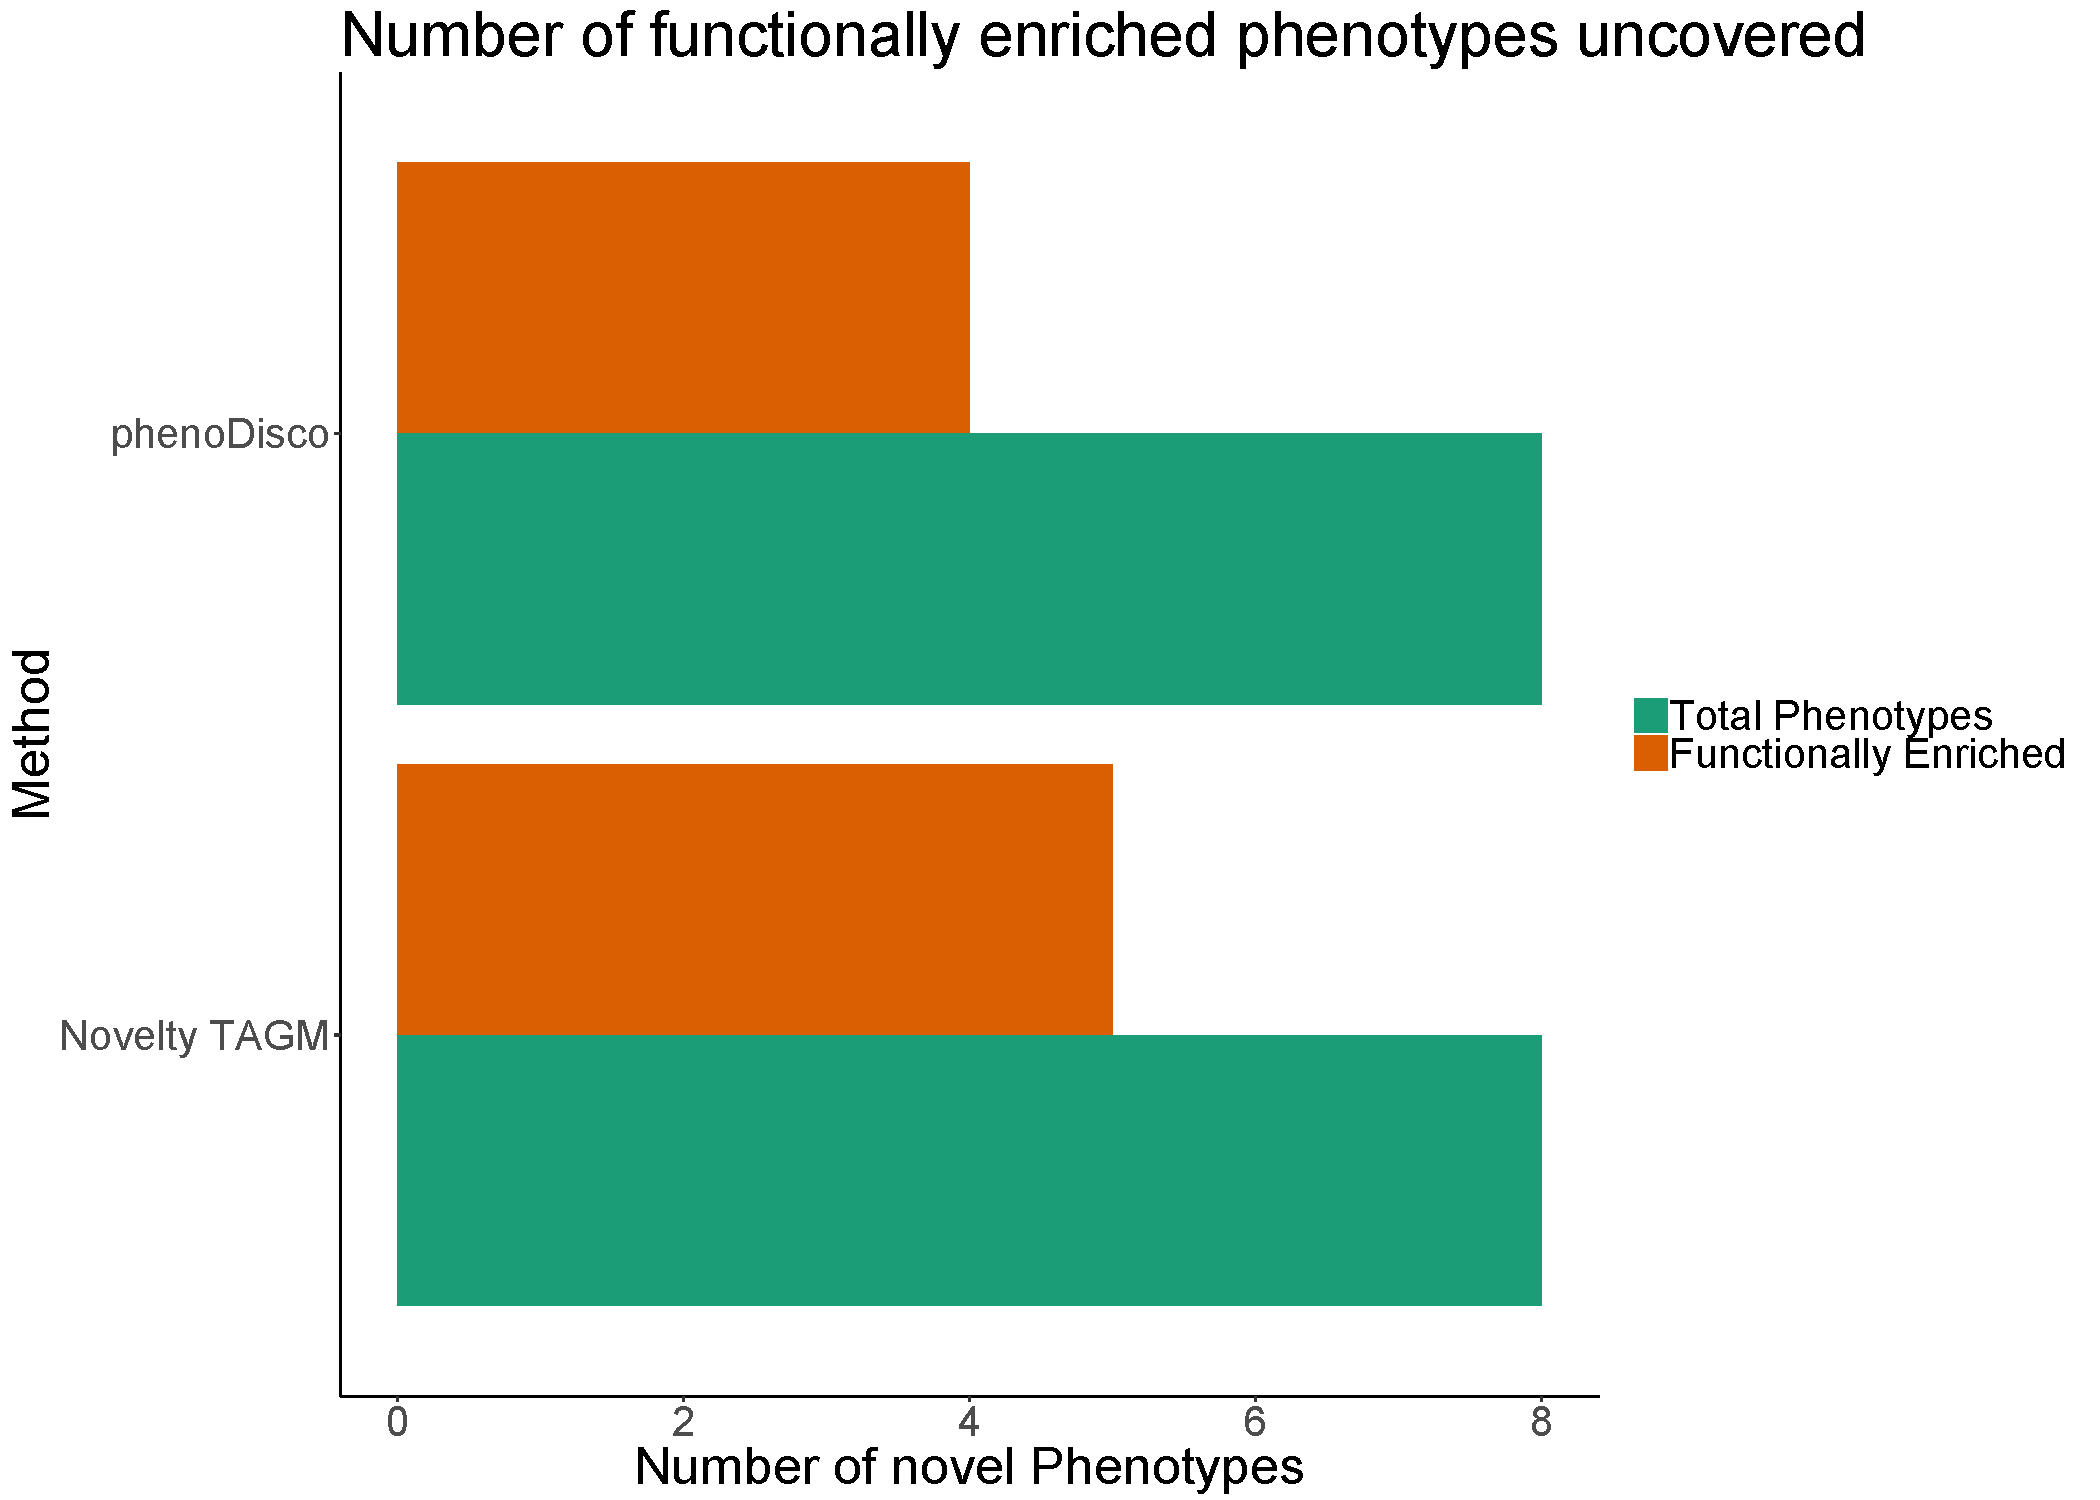
\includegraphics[height=2in]{phenonumhek}
	\caption{}
\end{subfigure}
	\begin{subfigure}[t]{0.5\textwidth}
	\centering
	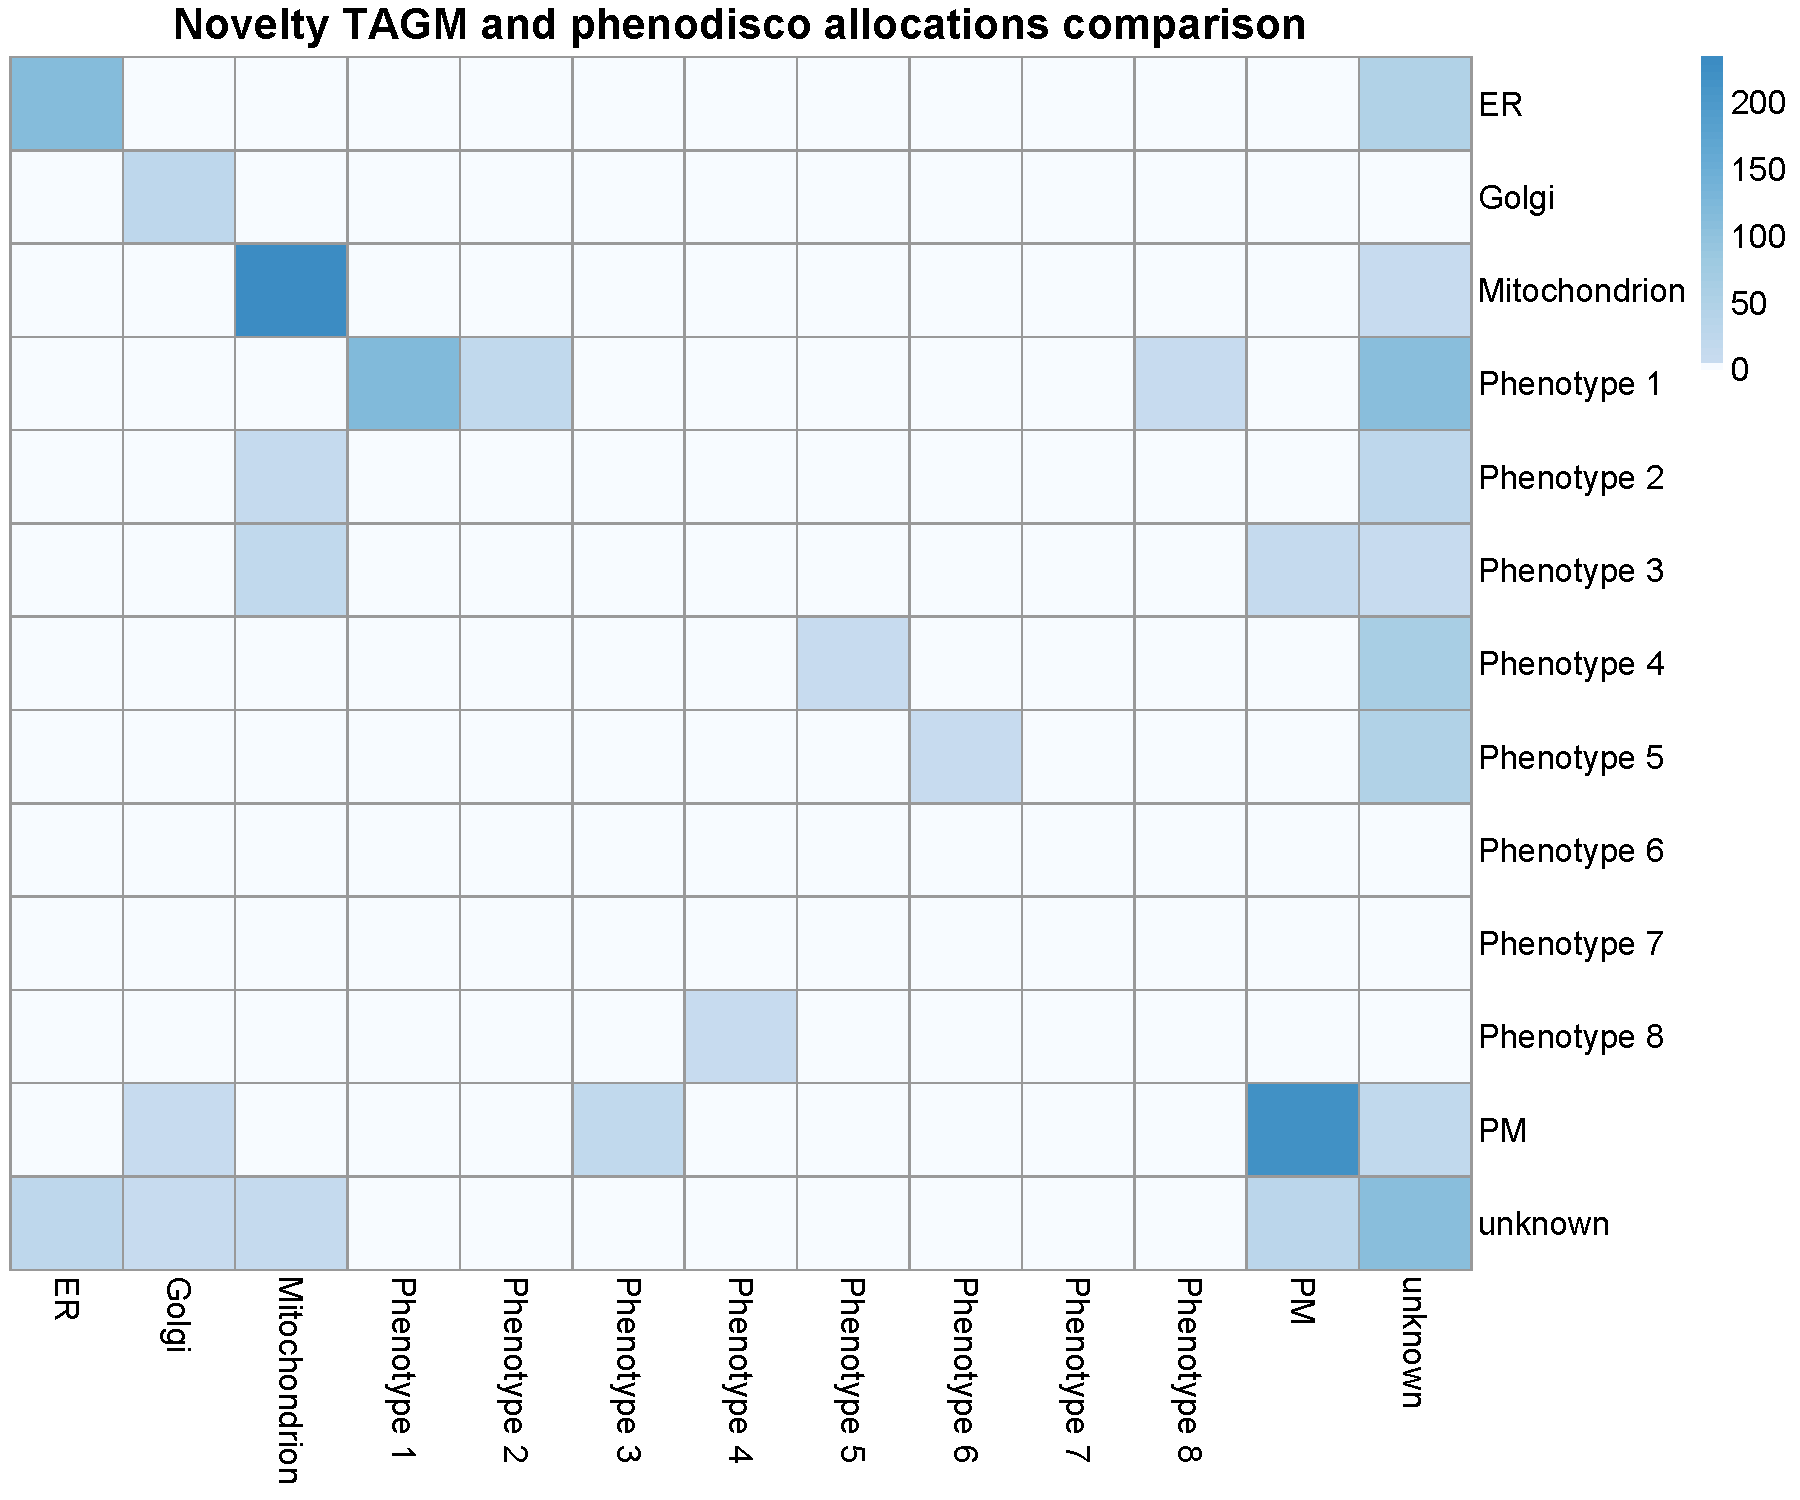
\includegraphics[height=2in]{hekcompare}
	\caption{}
\end{subfigure}
~
	\caption{(a) PCA plot showing marker proteins for the HEK-293 dataset. (b) PCA plot with phenotypes identified by \textit{phenoDisco}. (c) PCA plot with phenotypes identified by Novelty TAGM with pointer size scaled to discovery probability. (d, e) Barplots showing the number of proteins allocated to different phenotypes by \textit{phenoDisco} and Novelty TAGM respectively. (f) Barplot demonstrating the proportion of phenotypes with functional enrichment for both methods. (g) A heatmap showing the overlap between \textit{phenoDisco} and Novelty TAGM allocations.
	}
	\label{figure:phenodisco}
\end{figure}
\clearpage
\section{Improved annotation allows exploration of endosomal processes}
Given the information that the U-2 OS \textit{hyper}LOPIT dataset resolves an endosomal cluster, we perform a re-analysis of this dataset focusing on the endosomes. We curate a set of marker proteins for the endosomes and add these annotations to the U-2 OS \textit{hyper}LOPIT dataset. After which, we apply our Bayesian generative classifier TAGM to the data with this additional annotation \citep{Crook:2018}. Protein allocations to each subcellular niche can be visualised in the PCA plot of figure \ref{figure:u2os} (panel a). Figure \ref{figure:u2os} (panel c) demonstrates the increased number of protein that can be characterised by improved annotation of the U-2 OS cell line. Furthermore, we explore $8$ proteins with uncertain endosomal localisation, which can be visualised in each of the violin plots in \ref{figure:u2os} (panel d), where available, we compare with HPA immuno-staining.

Q92738 (RN-tre) is an intracellular trafficking protein involved in retrograde transport from the endocytic pathway to the Golgi apparatus \citep{Haas:2007}. RN-tre acts on Rab5, as a GTPase activating protein and in complex with the Eps8, for EGF dependant receptor internalisation \citep{Lanzetti:2000}. Additionally, RN-tre targets Rab43 for the regulation of Shiga toxin by transporting it from the early endosome to the trans-golgi network \citep{Fuchs:2007}. Here we observe a steady-state snapshot of the localisations of RN-tre with potential localisation to the endosome and plasma membrane.

Q15833 (STXBP2) is a protein of interest because genetic mutations are linked with adverse patient outcome of familial hemophagocytic lymphohistiocytosis type 5 (FHL5) \citep{Zur:2009, Pagel:2012} and is required for platelet secretion \citep{Al:2012}. The biological function of STXBP2 is to regulate vesicle to membrane fusion by mediatation of the SNARE complex \citep{Martin:2003, Sigismund:2012}. The endosomal/PM localisation of STXBP2 is thus inline with its biological role. 

P61020 (RAB5B), a monomeric G protein, is a constituent member of the RAS oncogene superfamily. RAB5B binds directly to EEA1 via the N-terminus and the C-terminal domain of EEA1 binds to the endosome, constituting direct evidence for endosomal localisation \citep{Callaghan:1999}. This is supported by its HPA localisation to vesicles (figure \ref{figure:u2os} (panel b)) and so the endosomal localisation observed here is unsurprising. 

O15498 (YKT6) is part of a SNARE complex which is involved with retrograde transport from the endosome to the Golgi apparatus \citep{Tai:2004}. We observed a mixed steady-state localisation of YKT6 between the cytosol and endosome. The cytosolic localisation is supported by the HPA annotation (figure \ref{figure:u2os} (panel b)) and endosomal localisation is further evidence of its role in vesicle docking in endocytosis.

Q9NZN3 (EHD3) is part of the EHD family of proteins that, through interaction with RAB11, regulate endocytic recycling \citep{Naslavsky:2006,George:2007}. HPA information (figure \ref{figure:u2os} (panel b)) and previous studies have also observed plasma membrane localisation \citep{George:2007}, suggesting a role for this protein in rapid recycling protein transport. 

P20339 (RAB5A), a small GTPase and key regulator of membrane trafficking, forms a complex with with the EEA1 C(2)H(2) zinc finger binding at the N-terminus \citep{Mishra:2010} and thus associates RAB5A with endosomal tethering. Potential localisation of RAB5A to the early endosome \citep{Fouraux:2004, Hunker:2006} and its role in endocytosis also permits the potential PM localisation observed here.

Q96L93 (KIF16B) is a highly dynamic kinesin-like plus end-directed microtubule-dependent motor protein involved in endosome transport and receptor recycling \citep{Hoepfner:2005}. Thus, a mixed localisation between endosome and PM is reflective of its biological roles, however HPA data clearly localises this protein to the Mitochondria (figure \ref{figure:u2os} (panel b)). This contradicts the supposed biological role of this protein, which arises from the uncertainty surrounding the specificity of the chosen antibody \citep{Thul:2017}.

Q8NHG (ZNRF2), a E3 ubiquitin ligase, which is a substrate of mTOR and interacts with the mTORC1 complex \citep{Hoxhaj:2016}. Previous studies have suggested endosomal, lysosomal and membrane localisation  for ZNRF2 \citep{Araki:2003, Hoxhaj:2016}. The localisation observed here is supportive of these previous studies.

\begin{figure}[h]
	\begin{subfigure}[t]{0.3\textwidth}
		\centering
		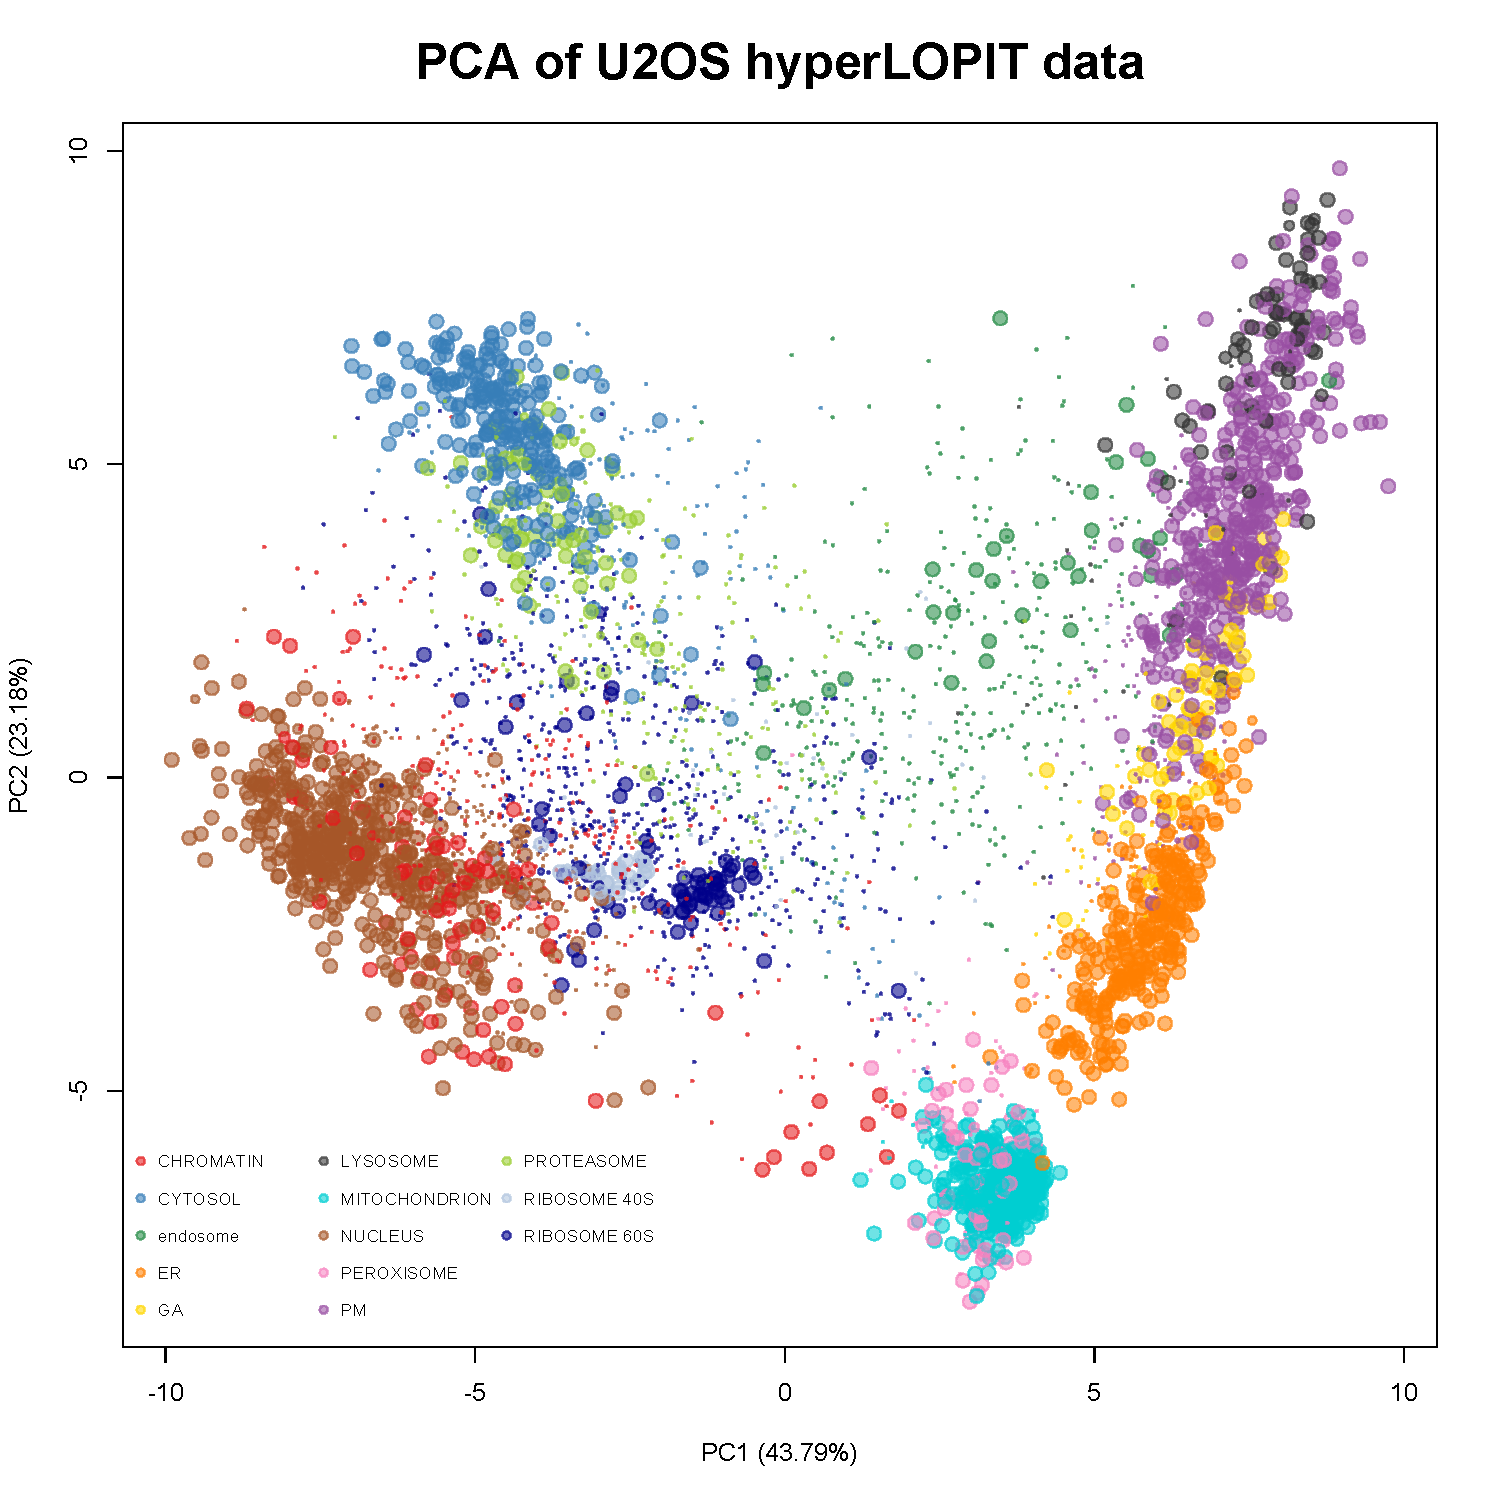
\includegraphics[height=2in]{u2ospcaF}
		\caption{}
	\end{subfigure}
	\begin{subfigure}[t]{0.3\textwidth}
	\centering
	\includegraphics[height=2in]{hpa2}
	\caption{}
	\end{subfigure}
	\begin{subfigure}[t]{0.3\textwidth}
	\centering
	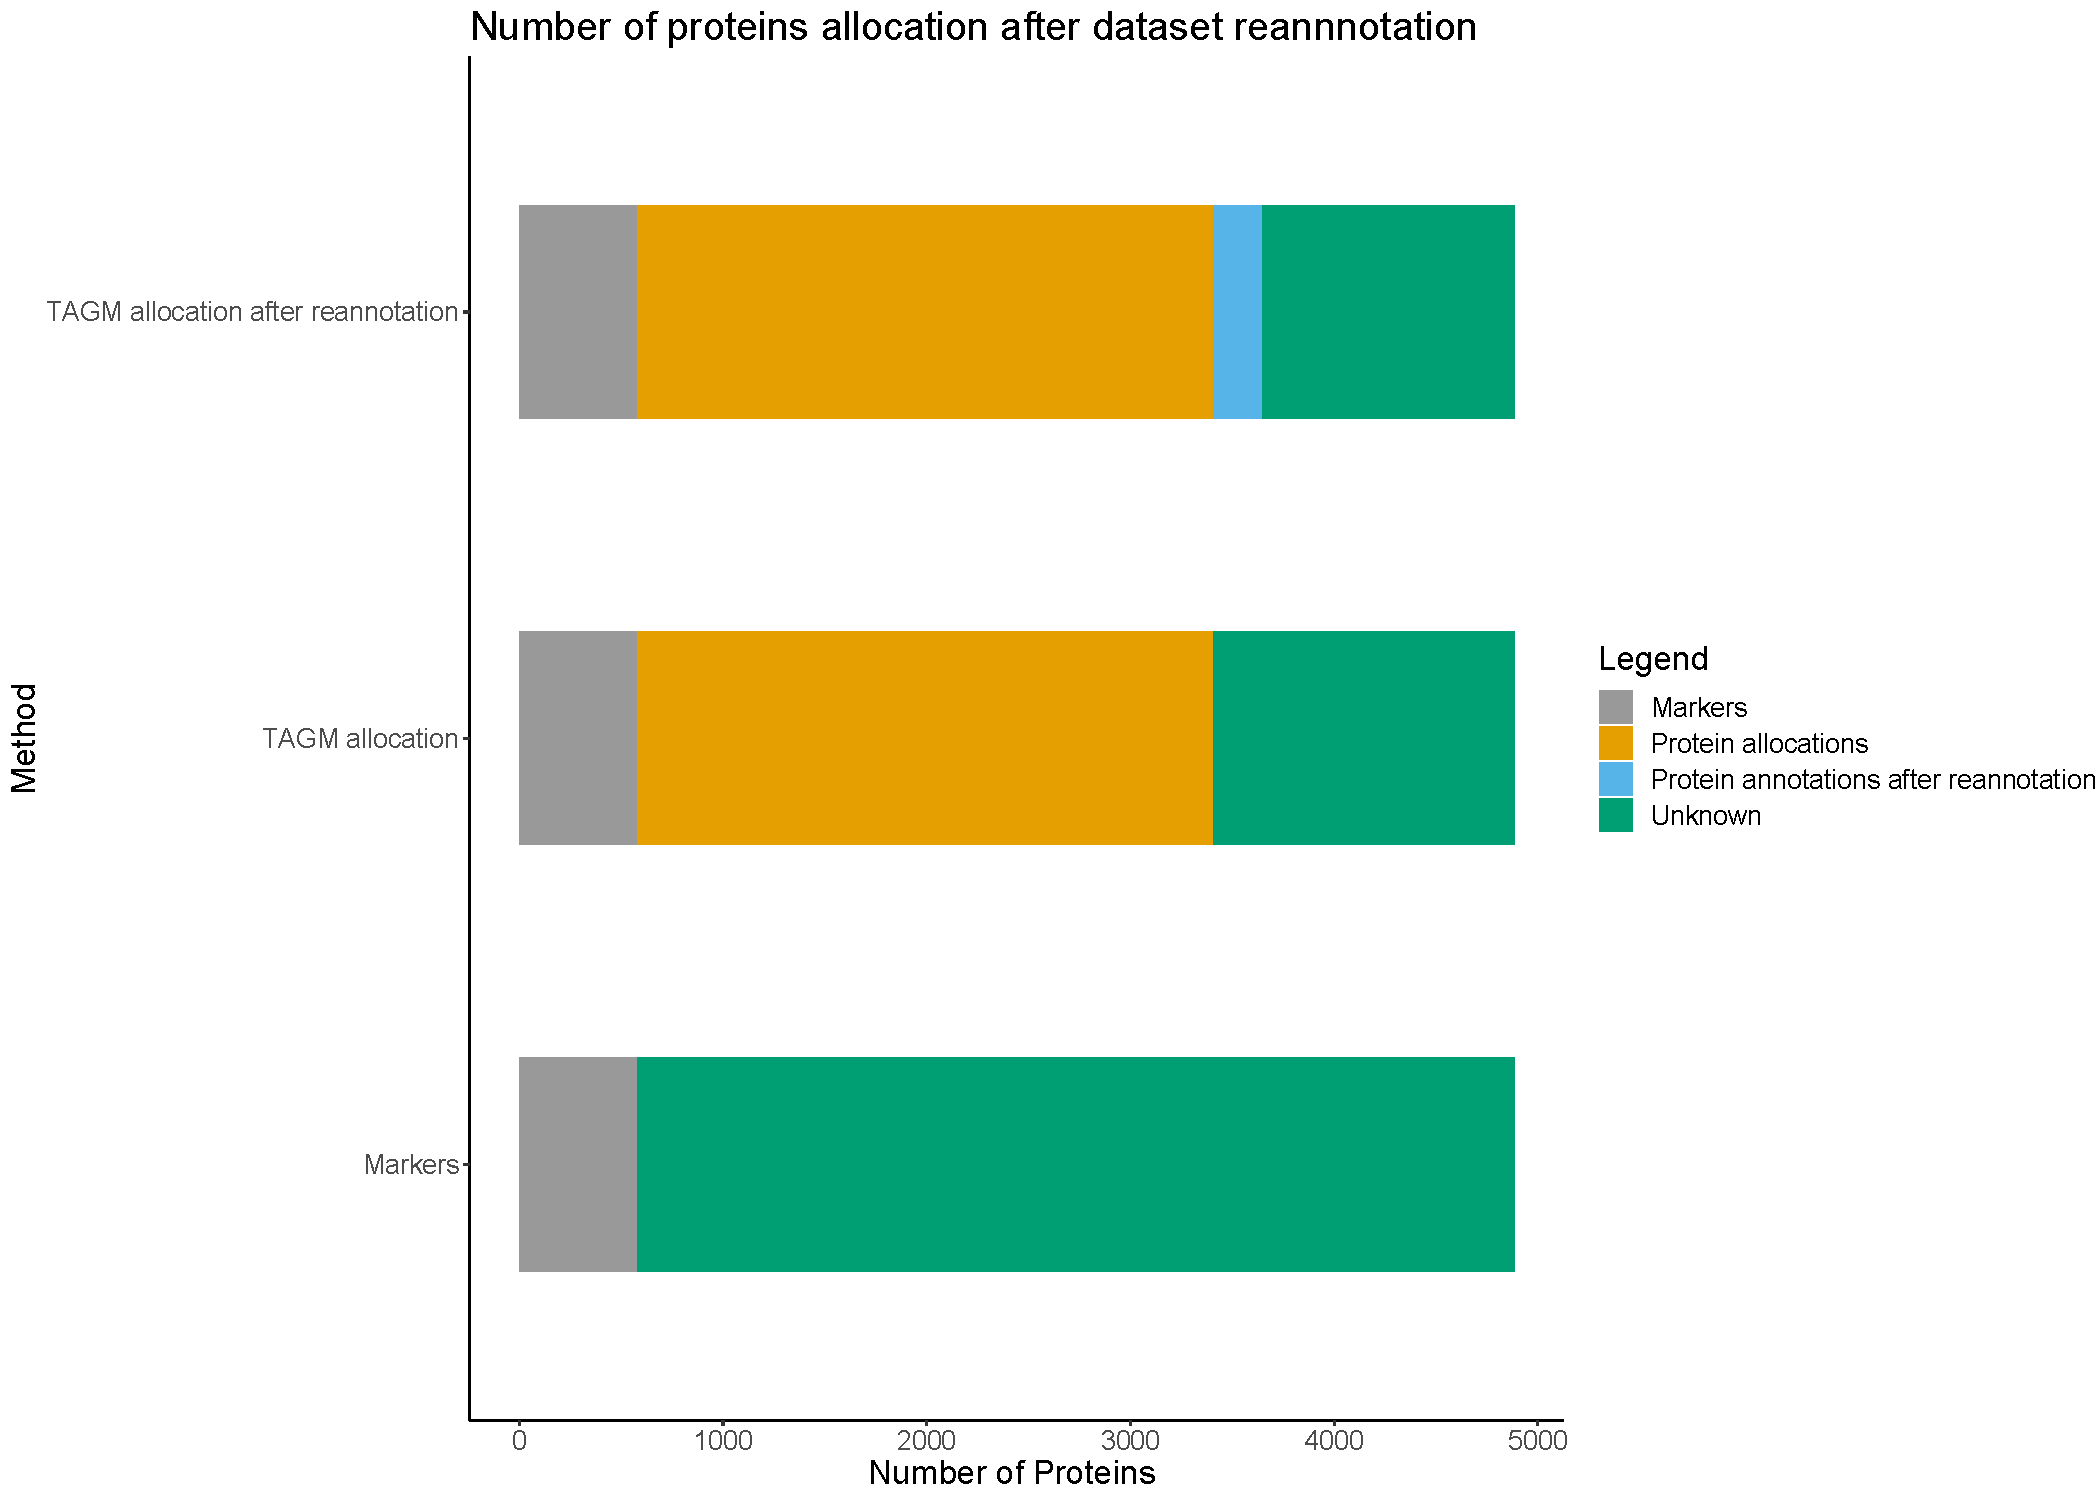
\includegraphics[height=2in]{summaryu2os}
	\caption{}
	\end{subfigure}
	~
	\begin{subfigure}[t]{1\textwidth}
		\centering
		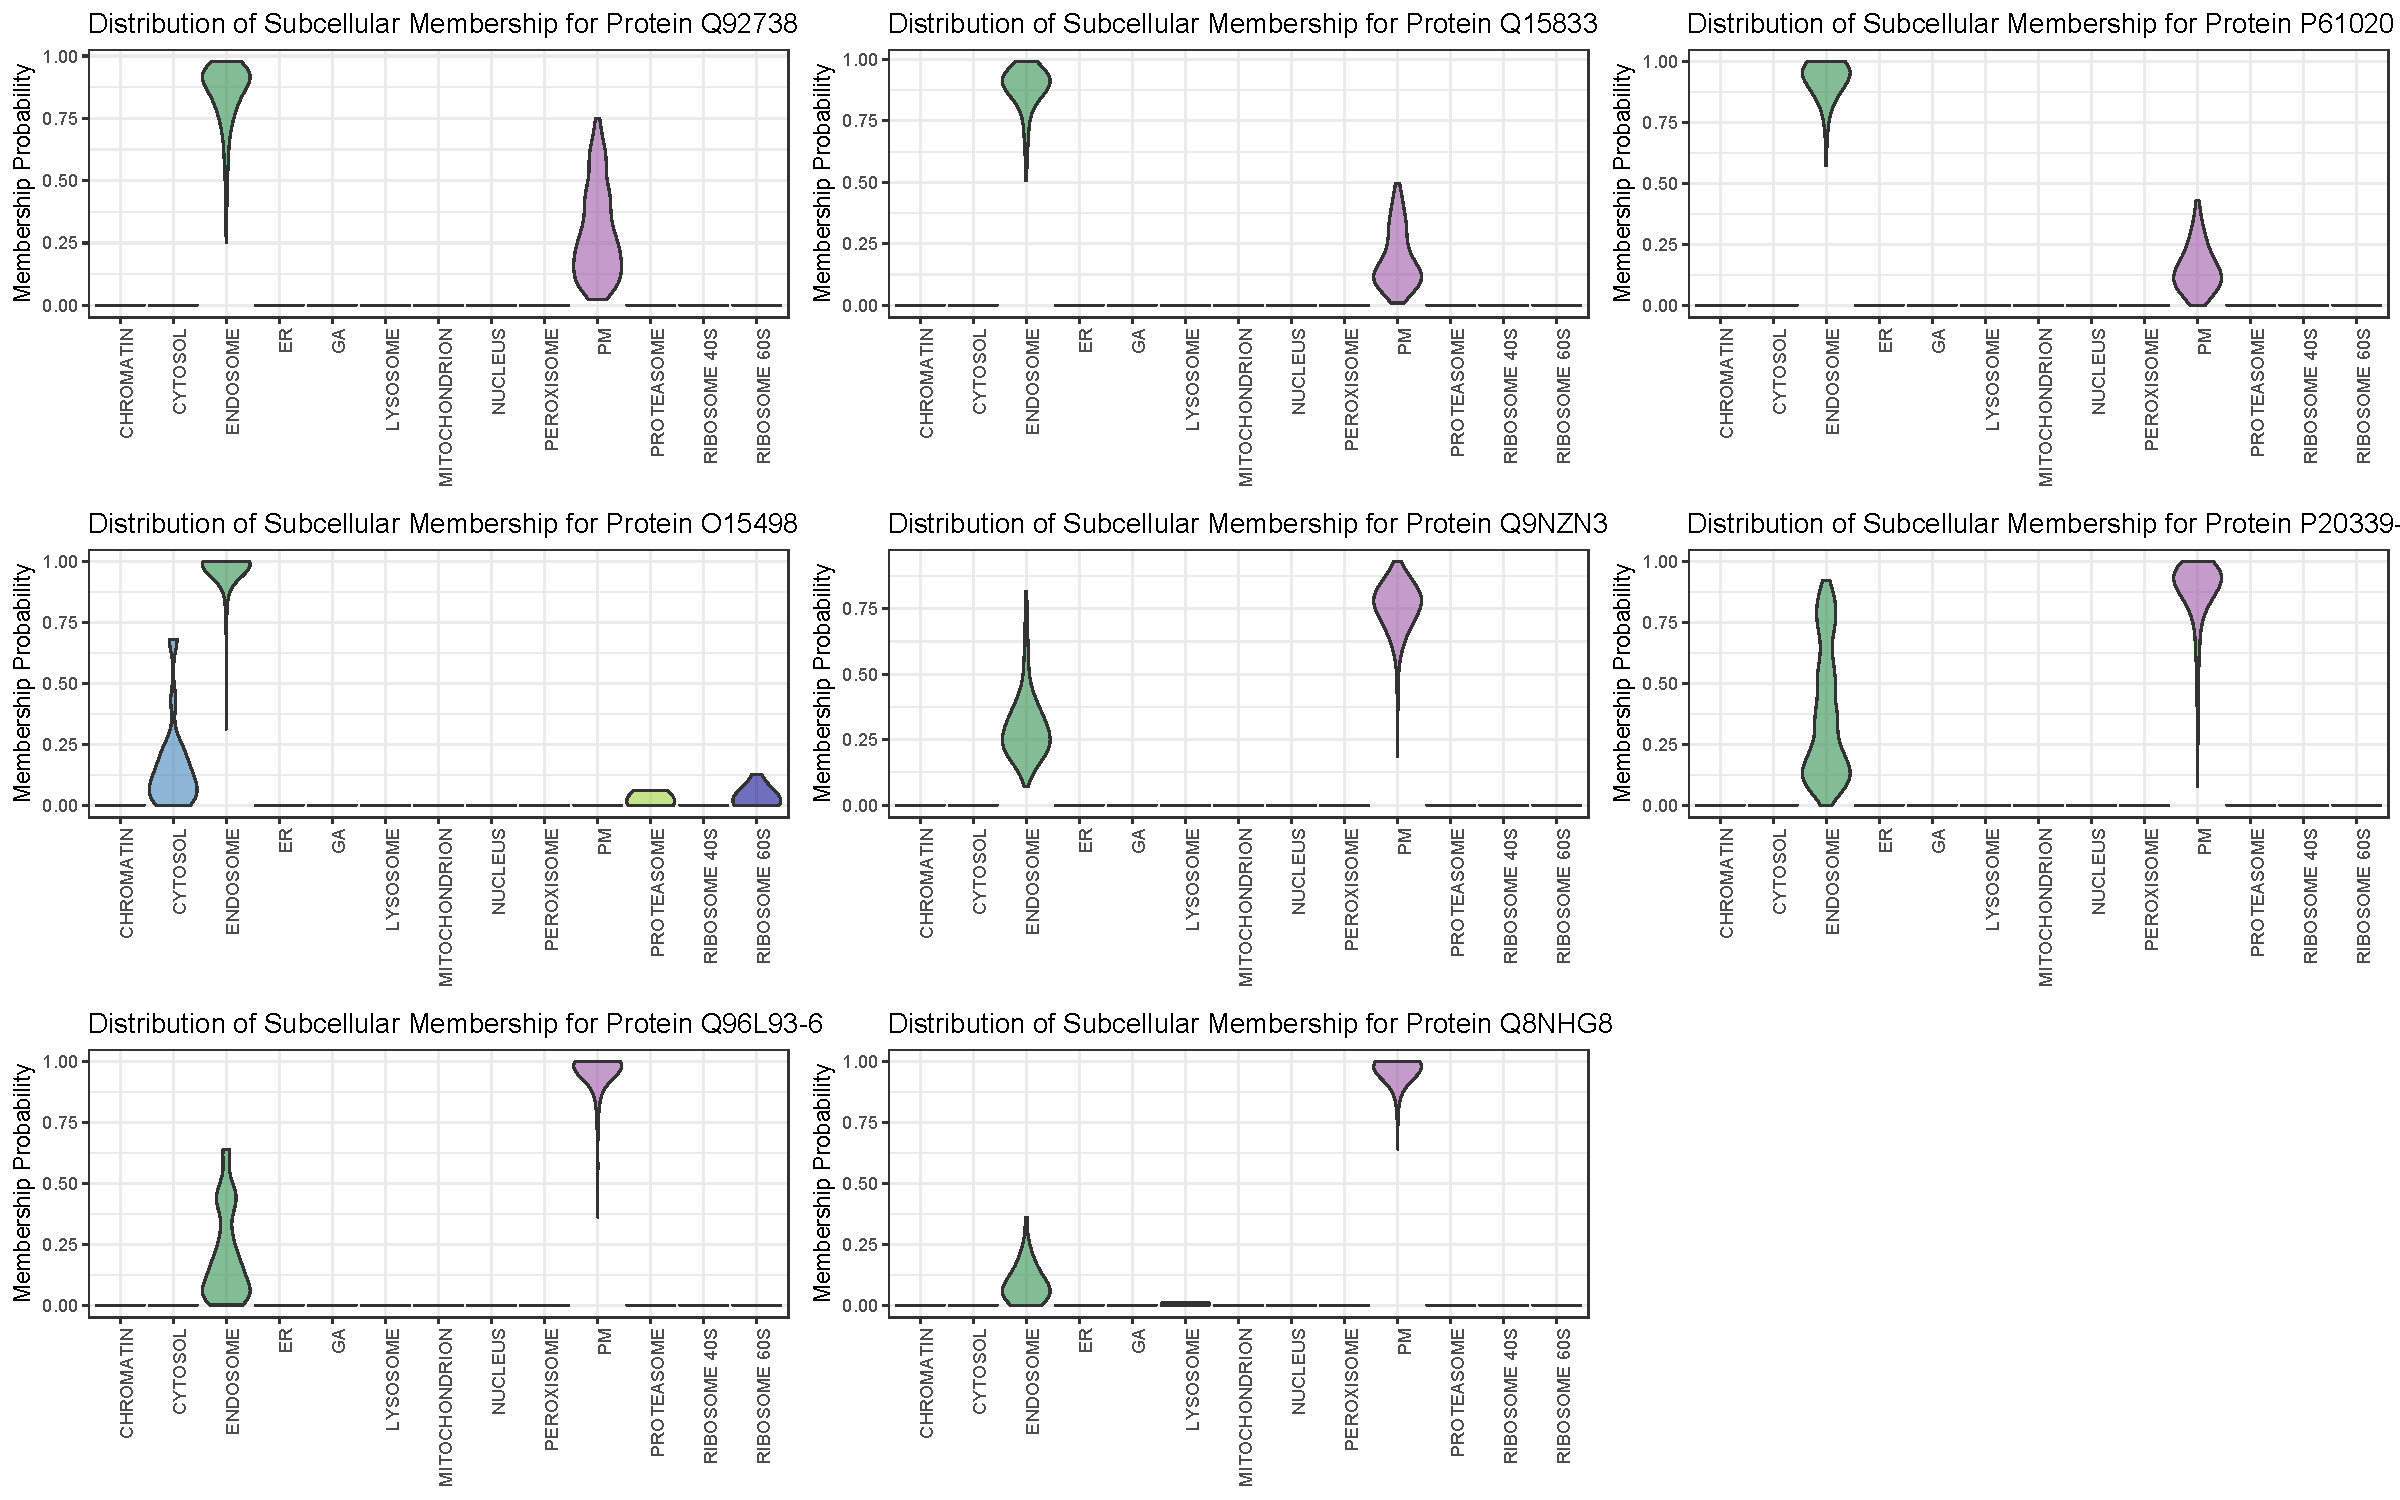
\includegraphics[height=4in]{endoViolin}
		\caption{}
	\end{subfigure}
	\caption{(a) PCA of U-2 OS \textit{hyper}LOPIT data with pointer scaled to localisation probability and outliers shrunk. Points are coloured according to their most probable organelle. (b) Immunofluorescence images and subcellular localisation annotation taken from the HPA database (https://www.proteinatlas.org/humanproteome/cell) for the proteins with UniProt accessions P61020, O15498, Q9NZN3, and Q96L93. The nucleus is stained in blue; microtubules in red, and the antibody staining targeting the protein in green. (c) A barplot representing the number of proteins allocated before and after re-annotation of the endosomal class. (d) Violin plots of full probability distribution of proteins to organelles, where each violin plot is for a single protein.
	}
	\label{figure:u2os}
\end{figure}
\clearpage 
\section{Discussion}
We have presented a semi-supervised Bayesian approach that simultaneously allows probabilistic allocation of proteins to organelles, detection of outlier proteins, as well as the discovery of novel sub-cellular structures. Our method unifies several approaches present in the literature, combining the ideas of supervised machine learning and unsupervised structure discovery. Formulating inference in a Bayesian framework allows for the quantification of uncertainty; in particular, the uncertainty in the number of newly discovered annotations.

Our proposed methodology allows us to interrogate individual proteins to see whether they belong to a newly discovered phenotype. Through the posterior similarity matrix we can visualise the global patterns in the uncertainty in phenotype discovery. We summarise this posterior similarity matrix into a single clustering by maximising the posterior expected adjusted rand index. This methodology infers the number of clusters supported by the data, in contrast to many ad-hoc approaches which require specification of the number of clusters.

Application of our method across $10$ different spatial proteomics acquired using diverse fractionation and MS data acquisition protocols and displaying varying levels of resolution revealed additional annotation in every single dataset. Our analysis recovered the chromatin-associated protein phenotype and validated experimental design for chromatin enrichment in \textit{hyper}LOPIT datasets. Our approach also revealed additional sub-cellular niches in the mESC \textit{hyper}LOPIT and U-2 OS \textit{hyper}LOPIT datasets.

Our method revealed resolution of $4$ sub-nuclear compartments in the U-2 OS \textit{hyper}LOPIT dataset, which was validated by Human Protein Atlas annotations. An additional endosome-enriched phenotype was uncovered and Novelty TAGM robustly identified an overlapping phenotype in U-2 OS LOPIT-DC data providing strong evidence for endosomal resolution. Further biologically relevant annotations were uncovered in these, as well as other, datasets. For example, a group of vesicle-associated proteins involved in transport from the ER to the early Golgi was identified in the yeast \textit{hyper}LOPIT dataset; resolution of the ribosomal subunit was identified in the fibroblast dataset, and separate nuclear, cytosolic and ribosomal annotations were identified in the DOM datasets.

A direct comparison with the state-of-the-art approach \textit{phenoDisco} demonstrates clear differences between the approaches. Novelty TAGM, a fully Bayesian approach, quantifies uncertainty in both the number of newly discovered phenotypes and the individual protein-phenotype associations - \textit{phenoDisco} provides no such information.

Improved annotation of the U-2 0S \textit{hyper}LOPIT data allowed us to explore endosomal processes, which have not previously been considered with this dataset. We compare our results directly to immunofluorescence microscopy-based information from the HPA database and demonstrate the value of orthogonal spatial proteomics approaches to determine protein sub-cellular localisation.

Thus, our method is widely applicable within the field of spatial proteomics and builds upon state-of-the-art approaches. The computational algorithms presented here are disseminated as part of the Bioconductor project \citep{Bioconductor::2004, Huber:2015} building on MS-based data structures provided in \cite{MSnbase:2012} and are available as part of the pRoloc suite, with all data provided in pRolocdata \citep{pRoloc:2014}.

During our analysis, we observed that the posterior similarity matrices have potential sub-clustering structures. Many known organelles and sub-cellular niches have sub-compartmentalisation, thus methodology to detect these sub-compartments is in preparation. Furthermore, we have observed that different experiments and different data modalities share information. Integrative approaches to spatial proteomics analysis are also desired. 

\section{Appendix}
\subsection{Handling label switching}
Bayesian inference in mixture models suffers from an identifiability issue known as \textit{label switching} - a phenomenon where the allocation labels can flip between runs of the algorithm \citep{Richardson::1997, Stephens:2000}. This occurs because of the symmetry of the likelihood function under permutations of these labels. We note that this only occurs in unsupervised or semi-supervised mixture models. This makes inference of the parameters in mixture models challenging. In our setting the labels for the known components do not switch, but for the new phenotypes label switching must occur. One standard approach to circumvent this issue is to form the so-called \textit{posterior similarity matrix} (PSM) \citep{fritsch::2009}. The PSM is an $N\times N$ matrix where the $(i,j)^{th}$ entry is the posterior probability that protein $i$ and protein $j$ reside in the same component. More precisely, if we let $S$ denote the PSM and $T$ denote the number of Monte-Carlo iterations then 
\begin{equation}
S_{ij} = P(z_i = z_j| X, \boldsymbol{\theta}, \boldsymbol{\pi} , \kappa, \epsilon, {\bf M}, V) \approx \frac{1}{T} \sum_{t = 1}^{T} \mathds{I}(z^{(t)}_i = z^{(t)}_j),
\end{equation}
where $\mathds{I}$ denotes the indicator function. The PSM is clearly invariant to label switching and so avoids the issues arising from the \textit{label switching} problem. 
\subsection{Summarising posterior similarity matrices}
To summarise the PSMs, we take the approach proposed by \cite{fritsch::2009}. They proposed the adjusted Rand index (AR) \citep{rand::1971, Hubert::1985}, a measure of cluster similarity, as a utility function and then we wish to find the allocation vector $\hat{z}$ that maximises the expected adjusted Rand index with respect to the true clustering $z$. Formally, we write
\begin{equation}
\hat{z} = \arg \max_{z^*} E[AR(z^*, z)|X, \boldsymbol{\theta}, \boldsymbol{\pi} , \kappa, \epsilon, {\bf M}, V],
\end{equation}
which is known as the Posterior Expected Adjusted Rand index (PEAR). One obvious pitfall is that this quantity depends on the unknown true clustering $z$. However, this can be approximated from the MCMC samples:
\begin{equation}
PEAR \approx \frac{1}{T} \sum_{t = 1}^{T}AR(z^*, z^{(t)}).
\end{equation}
The space of all possible clustering over which to maximise is infeasibly large to explore. Thus we take an approach taken in \cite{fritsch::2009} to propose candidate clusterings over which to maximise. Using hierarchical clustering with distance $1 - S_{ij}$, the PEAR criterion is computed for clusterings at every level of the hierarchy. The optimal clustering $\hat{z}$ is the allocation vector which maximises the PEAR.
\subsection{Details of MCMC}
The MCMC algorithm use in \cite{Crook:2018} is insufficient to handle inference of unknown phenotypes. A collapsed Gibbs sampler approach is used, but a number of modifications are made. Firstly, to accelerate convergence of the algorithm half the proteins are initial allocated randomly amongst the new phenotypes. Secondly, the parameters for the new phenotypes are proposed from the prior. Throughout the same default prior choices are used as in \cite{Crook:2018}.
\subsection{Summary of convergence diagnostics}
We provide a summary of convergence diagnostics using parallel chains analysis \citep{Gelman:1992}. We compute the number of proteins allocated to the outlier component at each iteration of the Markov-chain and monitor this quantity for convergence. The $\hat{R}$ statistic between parallel chains in then computed and reported in the table below. A value of $\hat{R} < 1.2$ indicates convergence.
\begin{table}[h]
	\centering
	\footnotesize
	\begin{tabular}{ |p{5cm}|p{3cm}|p{2cm}|p{4cm}|  }
		\hline
		\multicolumn{4}{|c|}{Convergence diagnostics for MCMC} \\
		\hline
		\vfill\hfil Dataset & \vfill\hfil Protocol & \vfill\hfil$\hat{R}$ & \vfill\hfil Upper confidence Interval \vfill\hfil $\hat{R}$   \\
		\hline
		\hline
		mESC  & \textit{hyper}LOPIT&\vfill\hfil 1.03 & \vfill\hfil 1.15 \\
		\hline
		U-2 OS &\textit{hyper}LOPIT & \vfill\hfil 1.00  & \vfill\hfil 1.00\\
		\hline
		U-2 OS &LOPIT-DC  & \vfill\hfil 1.02&\vfill\hfil 1.06\\
		\hline
		\textit{S. cerevisiae} &\textit{hyper}LOPIT & \vfill\hfil 1.00 & \vfill\hfil 1.01\\
		\hline
		HCMV-infected fibroblast& Temporal LOPIT &  \vfill\hfil 1.01 & \vfill\hfil 1.02 \\
		\hline
		HCMV mock fibroblast& Temporal LOPIT &  \vfill\hfil 1.03 & \vfill\hfil 1.08 \\
		\hline
		HeLa \citep{Itzhak:2016}& DOM &  \vfill\hfil 1.07 & \vfill\hfil 1.21 \\
		\hline
		Mouse primary neurons & DOM &  \vfill\hfil 1.04 & \vfill\hfil 1.13 \\
		\hline
		HeLa \citep{Hirst:2018} & DOM &\vfill\hfil 1.02 & \vfill\hfil 1.06 \\
		\hline
		HEK-293 &LOPIT &  \vfill\hfil 1.00 & \vfill\hfil 1.01 \\
		\hline
		\hline
	\end{tabular}
	\caption{A table reporting convergence diagnostics for MCMC analysis}
	\label{table:mcmcconvergence}
\end{table}
 



\clearpage
\bibliographystyle{natbib}
\bibliography{BayesProt}
\end{document}
